\documentclass{article}

\usepackage[utf8]{inputenc}
\usepackage[margin=0.75in]{geometry}
\usepackage{amsmath,amssymb,amsfonts,amsthm}
\usepackage{bm}
\usepackage{graphicx}
\usepackage{booktabs}
\usepackage{multirow}
\usepackage{longtable}
\usepackage{subcaption}
\usepackage{hyperref}
\usepackage{xcolor}
\usepackage{cite}
\usepackage{cleveref}
\usepackage{pdflscape}

\hypersetup{
    colorlinks=true,
    linkcolor=blue,
    citecolor=blue,
    urlcolor=blue
}

% Mathematical Operators and Definitions
\newcommand{\real}{\mathbb{R}}
\newcommand{\tensor}[1]{\bm{\mathcal{#1}}}
\newcommand{\mat}[1]{\mathbf{#1}}
\newcommand{\vc}[1]{\bm{#1}}
\newcommand{\inner}[2]{\langle #1, #2 \rangle}
\newcommand{\norm}[1]{\| #1 \|}
\newcommand{\Ltwo}{L^2(\Omega)}

\title{\textbf{A Multi-Model Non-Intrusive Reduced-Order Framework for Parametric Erosion Prediction via Kinematic Cross-Moment Compression}}

\author{\textbf{Animesh Yadav, Rajesh K. Shukla}\\[0.5em]
\small{\textit{Department of Mechanical Engineering, Thapar Institute of Engineering and Technology, Patiala, Punjab 147004, India}}}

\date{\today}

\begin{document}

\maketitle

\begin{abstract}
High-fidelity Eulerian--Lagrangian simulations of solid particle erosion in curved pipes require hours of compute per operating point, preventing rapid parameter sweeps and real-time wear assessment. Existing reduced-order models (ROMs) speed up these evaluations, yet they are typically trained on a single, fixed empirical erosion formula (e.g., Oka or Finnie). Changing the material law or target hardness then requires a complete retrain of the surrogate. Here, we present a non-intrusive reduced-order framework that avoids this model-locking by approximating the underlying particle collision kinematics instead of scalar wear rates. Specifically, we project and compress 23 Eulerian boundary cross-moments ($\mathbb{E}[V_p^u \sin^v\alpha_p \cos^w\alpha_p]$) across the pipe surface.

Using 372 high-fidelity CFD-DPM cases of $90^\circ$ elbows over three bend ratios ($R/D \in \{1.5, 2.0, 5.0\}$), five Reynolds numbers, five density ratios, and six particle diameters in the inertial regime ($St > 1$), we evaluate a hybrid compression scheme. Linear Proper Orthogonal Decomposition (POD) and Mode-1 tensor unfolding SVD are combined with block-wise Convolutional Autoencoders (CNN-AE) to handle both broad convective transport and localized impact craters. An anisotropic Gaussian Process Regression (GPR) surrogate maps four dimensionless $\Pi$-groups to the compressed latent space, evaluating full 2D wear topographies in roughly $2\,\mathrm{ms}$ ($R^2 > 0.99$ on primary kinematic fields). Because kinematics are decoupled from material damage laws, the resulting surrogate evaluates multiple empirical models post-hoc---exactly matching Finnie and closely approximating Oka, McLaury, and Arabnejad---without retraining.
\end{abstract}

\textbf{Keywords:} Reduced-Order Modeling (ROM), Solid Particle Erosion, Convolutional Autoencoder, Gaussian Process Regression, Computational Fluid Dynamics (CFD), Multiphase Flow.

\section{Introduction}
\label{sec:introduction}

Solid particle erosion in piping components is a leading source of mechanical failure in slurry transport, subsea hydrocarbon production, and pneumatic conveying lines \cite{parsi2014review,kang2024erosive,zahedi2018,othman2024integration,chen2024novel}. Abrasive slurries in mineral processing and dredging networks erode pipe walls rapidly \cite{sinha2017review,espinozajara2025,clark1992,desale2009}, while fly-ash causes pipe punctures in coal-fired power plants \cite{wang2022numerical,kang2024erosive}. The same mechanism is applied intentionally in abrasive jet finishing for optical polishing \cite{chen2017ajp}. In all these piping layouts, $90^\circ$ elbows are inevitable, yet the sharp turn in fluid momentum causes severe localized wall thinning---often producing wear rates up to 50 times greater than in straight pipes \cite{lin2015effect,chen2004cfd,yu2025ocean,mondal2022burst,mahmoudi2025erosion}.

Wear in elbows results from secondary flow structures interacting with suspended particulates \cite{clark1992,desale2009,kang2024erosive,espinozajara2025}. The radial pressure gradient in the bend establishes a pair of counter-rotating Dean vortices across the pipe cross-section. At the wall, material removal depends on impact angle: shallow grazing collisions ($\alpha < 30^\circ$) cause micro-machining and plowing, while near-normal impacts ($\alpha \approx 90^\circ$) cause plastic deformation, subsurface fatigue, and platelet spalling \cite{finnie1960erosion,bitter1963,bellman1981erosion,albukhaiti2007}. The resulting spatial wear footprint depends strongly on the particle Stokes number, $St = (\rho_p d_p^2 U_{\mathrm{in}})/(18 \mu_f D)$ \cite{hajisharifi2023non,mahmoudi2025erosion}:
\begin{itemize}
    \item \textbf{Low-Inertia Sweeping Regime ($St < 0.1$):} Fine particles track fluid streamlines and Dean circulations, distributing light wear across the pipe crowns ($\theta \approx \pm \pi/2$) \cite{espinozajara2025}.
    \item \textbf{High-Inertia Ballistic Impingement Regime ($St \gg 1$):} Heavy particles cross streamlines ballistically, slamming into the outer extrados wall ($\theta = 0$) and forming deep craters \cite{clark1992,chen2004cfd,mahmoudi2025erosion}.
\end{itemize}

\textcolor{red}{Historically, modeling solid particle erosion started with semi-empirical wear equations. Finnie \cite{finnie1960erosion} proposed early models for ductile micro-machining, while Bitter \cite{bitter1963} accounted for both cutting and plastic deformation. These early works usually modeled erosion as a simple power-law function of impact velocity ($E \propto V^n$, $n \approx 1.7$--$2.6$) and particle size ($d_p^m$) \cite{clark1992,elkholy1983prediction,desale2009}. Over time, researchers expanded these equations to include target material hardness, particle shape, and non-monotonic impact angle curves for different alloys. This led to the standard engineering wear models widely used today, such as those by McLaury and Shirazi \cite{mclaury1996,mclaury1999,chen2004cfd}, Ahlert \cite{ahlert1994}, Oka et al.~\cite{oka2005erosion1,oka2005erosion2}, and Arabnejad et al.~\cite{arabnejad2015}.}

\textcolor{red}{Once computational fluid dynamics (CFD) matured, the Eulerian--Lagrangian (CFD--DPM) approach became the standard way to map out 3D erosion patterns in pipes \cite{chen2004cfd,peng2016numerical,parsi2017cfd,singh2019modeling,wee2019cfd,wang2021experimental,mahmoudi2025erosion}. In these models, the fluid is typically solved using Reynolds-Averaged Navier--Stokes (RANS) or Large Eddy Simulation (LES) \cite{launder1972lectures}, and the solid phase is tracked by simulating hundreds of thousands of individual particle trajectories. To account for turbulence, most studies use Discrete Random Walk (DRW) models alongside empirical wall restitution coefficients (like Grant and Tabakoff \cite{grant1975}). Validation studies by Solnordal et al.~\cite{solnordal2015} and Parsi et al.~\cite{parsi2014review} have shown that CFD--DPM does a very good job at predicting the location and depth of the primary wear scar in $90^\circ$ elbows. The main drawback, however, is the computational cost. A single 3D CFD--DPM simulation often takes $6$--$8$ CPU hours to run. This makes it practically impossible to use CFD directly for real-time structural monitoring, life extension planning, or large-scale design optimization \cite{wang2022numerical,mondal2022burst}.}

\textcolor{red}{To get around these slow solve times, researchers have recently turned to machine learning (ML) surrogates and reduced-order models (ROMs) (see Jindal et al.~\cite{jindal2026artificial} for a recent review). Early attempts mostly focused on predicting a single scalar value for the wear rate using tools like Random Forest regression \cite{zahedi2018,yang2021experimental}, swarm-optimized algorithms, gradient-boosted trees \cite{wang2022solid,zhang2021solid}, or Extreme Learning Machines \cite{wang2022numerical,liu2021exploration}. More recently, the focus has shifted to predicting the actual spatial distribution of the wear. Pandya et al.~\cite{pandya2020cfd} and Othman et al.~\cite{othman2024integration} used CFD-trained Artificial Neural Networks (ANN), while Ma et al.~\cite{ma2024mechanism}, Chen et al.~\cite{chen2024novel}, and Shojaie et al.~\cite{shojaie2023method,shojaie2024comprehensive} developed physics-guided Gaussian Process Regression (GPR) models that also provide uncertainty estimates. Pushing into deep learning, Li et al.~\cite{li2026cfd} recently trained a CNN--LSTM network optimized by a Coati Optimization Algorithm (COA) to predict time-dependent wear in slurry elbows.}

\textcolor{red}{At the same time, spatial projection techniques like Proper Orthogonal Decomposition (POD) \cite{sirovich1987turbulence,rozza2008reduced,quarteroni2015reduced}, tensor decompositions (HOSVD/Tucker) \cite{tucker1966some,lathauwer2000multilinear,barragan2025motif,alsayyari2019}, and convolutional autoencoders (CNN-AE) \cite{fresca2021pod,xiao2019,murata2020nonlinear,hajisharifi2023non,jiang2023data,garcia2016data} have become very popular for speeding up single-phase CFD and other PDE systems \cite{brunton2019data}. But despite all this progress in CFD and ML surrogates, there are still a few major problems with how the community currently models erosion:}
\begin{enumerate}
    \item \textbf{Loss of Spatial Information (0D Reduction):} Several ML approaches \cite{zahedi2018,othman2024integration,wang2022numerical,wang2022solid,zhang2021solid} collapse the boundary collision field into a single scalar value (such as peak penetration rate or total mass loss). This discards the spatial wear distribution, crater width, axial elongation, and downstream ricochet zones needed for structural integrity checks and ASME B31G fitness-for-service assessments.
    
    \item \textbf{The Model-Locking Dilemma:} All existing spatial erosion surrogates in the literature \cite{ma2024mechanism,chen2024novel,li2026cfd,pandya2020cfd} are trained directly on the scalar output of a single pre-selected empirical wear equation (e.g., Oka or DNV). Because erosion parameters depend heavily on target metallurgy, hardness, erodent angularity, and fluid chemistry \cite{parsi2014review,kang2024erosive,jindal2026artificial}, altering the pipe alloy or employing a newly calibrated wear law completely invalidates the trained surrogate, necessitating a full re-computation of the CFD--DPM database and complete model retraining.
    
    \item \textbf{Extreme Spatial Sparsity and High-Stokes Craters:} Wear in elbows is heavily localized: over $70\%$ of the pipe surface (the intrados) receives practically zero particle collisions, while damage concentrates in a small patch on the extrados ($\sim 30\%$ area). Standard unweighted POD and monolithic autoencoders minimize global $L_2$ error, causing them to fit the broad zero-wear regions while underpredicting sharp peak depths in heavy ballistic flows ($St \gg 1$).
    
    \item \textbf{Multi-Channel Optimization Stalling:} Jointly compressing high-dimensional multi-physics fields through a single monolithic convolutional bottleneck causes slower training convergence and higher terminal loss, as shown in our ablation tests (Section~\ref{sec:fwcnn_vs_unweighted}).
\end{enumerate}

To address these limitations, this paper introduces a non-intrusive reduced-order framework that operates on fundamental particle collision kinematics rather than pre-computed scalar wear rates. By extracting and compressing 23 Eulerian boundary cross-moments ($\mathbb{E}[V_p^u \sin^v\alpha_p \cos^w\alpha_p]$) alongside impact frequencies, we decouple fluid-particle dynamics from surface wear equations, allowing instantaneous, post-hoc evaluation of diverse erosion formulations without retraining the surrogate.

\subsubsection*{Representable Function Class and Approximation Error}

\begin{table}[htpb]
\centering
\caption{Classification of erosion formulations and their representability within the selected 23-moment kinematic basis.}
\label{tab:representability}
\small
\resizebox{\linewidth}{!}{%
\begin{tabular}{lllll}
\toprule
\textbf{Erosion Model} & \textbf{Velocity Dependence} & \textbf{Angular Dependence} & \textbf{Exactly Representable?} & \textbf{Approximation Required?} \\
\midrule
Finnie & $V^2$ & $\sin(2\alpha), \cos^2\alpha$ & Yes & No \\
Oka & $V^{2.338}$ & $f(\alpha)$ non-polynomial & No (Approximated via basis) & Yes (Velocity \& Angle) \\
McLaury & $V^{1.73}$ (mapped to $V^2, V^1$) & $f(\alpha)$ piecewise poly & No (Approximated via basis) & Yes (Velocity \& Angle) \\
Arabnejad & $V^{2.41}, V^2$ & $f(\alpha)$ piecewise cutting/def. & No (Approximated via basis) & Yes (Velocity \& Angle) \\
Withheld Model & $V^{2.338}$ & $\sin^{1.5}\alpha (1-\cos\alpha)^{0.5}$ & No & Yes \\
\bottomrule
\end{tabular}%
}
\end{table}

The 23-moment basis exactly represents erosion formulations whose mathematical form falls within the span of the retained polynomials. Models outside this space are evaluated through continuous projection onto the basis, introducing a representation error:
\begin{equation}
    \mathbb{E}[g(V_p, \alpha_p)] = \sum_{k=1}^{23} c_k M_k, \quad \text{where } M_k = \mathbb{E}[V_p^{u_k} \sin^{v_k}\alpha_p \cos^{w_k}\alpha_p]
    \label{eq:exact_representation}
\end{equation}
This exact representation holds for polynomial-separable models $g(V,\alpha) = \sum_{u,v,w} A_{u,v,w} V^u \sin^v\alpha \cos^w\alpha$ with velocity powers $u \in \{1, 2, 2.5, 3\}$ and trigonometric powers $v,w \in \{0,1,2,3\}$, which includes Finnie. Formulations with non-polynomial angular functions or fractional exponents (e.g., Oka, McLaury, and Arabnejad) are projected onto the polynomial basis prior to taking the expectation over the particle ensemble:
\begin{equation}
    \mathbb{E}[g(V_p, \alpha_p)] \approx \sum_{k=1}^{23} c_k M_k + \epsilon_g
    \label{eq:approx_representation}
\end{equation}
Here $\epsilon_g$ is the truncation error from terms not spanned by the basis. In practice, the 23 moments were chosen by analyzing the velocity and angular dependencies in the Oka, Finnie, McLaury, and Arabnejad equations, augmented with higher powers ($V^3$, $\sin^3\alpha$) to ensure broad coverage.

The primary contributions of this work are:
\begin{enumerate}
    \item[(i)] \textbf{Kinematic Cross-Moment Abstraction:} We introduce a functional-basis formulation that represents particle wall impacts via 23 Eulerian cross-moments spanning velocity powers ($V^u$, $u \in \{1,2,2.5,3\}$), impact angle terms ($\sin^v\alpha$, $\cos^w\alpha$), and collision frequencies. This permits rapid post-hoc evaluation of diverse wear laws (exact for Finnie, approximate for Oka, McLaury, Arabnejad) without surrogate retraining.
    
    \item[(ii)] \textbf{Non-Intrusive Spatial Surrogate:} We construct a reduced-order model mapping four dimensionless $\Pi$-groups to 2D spatial fields of all 23 cross-moments using Gaussian Process Regression with ARD Mat\'ern-5/2 kernels, evaluating full surface wear in approximately $2\,\mathrm{ms}$.
    
    \item[(iii)] \textbf{Linear vs. Nonlinear Compression Benchmark:} We evaluate Snapshot POD, spatially weighted W-POD, Mode-1 tensor unfolding SVD, and custom frequency-weighted block-wise CNN-AEs across clustered variable groups. We show that linear W-POD is highly effective for coupled velocity-angle moments (Blocks 1--3), whereas block-wise CNN-AEs improve accuracy for continuous convective velocity fields (Block 4) and difficult uncoupled moments (Block 5).
    
    \item[(iv)] \textbf{Pipe-Conforming Curvilinear Mapping:} We establish an analytical coordinate transformation $(s_{\mathrm{norm}}, \theta)$ that maps $90^\circ$ elbows of varying curvature ratios ($R/D \in [1.5, 5.0]$) onto a canonical 2D computational grid $[0, 2] \times [-\pi, \pi]$, standardizing spatial topologies across design geometries.
    
    \item[(v)] \textbf{CFD Validation and Multi-Regime Verification:} The CFD-DPM setup is validated against multi-planar erosion depth measurements from Solnordal et al.~\cite{solnordal2015}. The NI-ROM surrogate is then tested on 75 locked out-of-sample CFD cases spanning standard elbows, long-radius bends, and heavy ballistic regimes ($St \in [1, 327]$).
\end{enumerate}

The manuscript is structured as follows. Section~\ref{sec:methodology} presents the mathematical formulation of the cross-moment abstraction, curvilinear mapping, data conditioning, spatial modal decompositions, and GPR surrogate. Section~\ref{sec:cfd_database} outlines the physical governing equations, CFD-DPM setup, mesh verification, experimental validation against Solnordal et al.~\cite{solnordal2015}, and dimensionless parameter space design. Section~\ref{sec:results} discusses modal convergence, autoencoder training dynamics, out-of-sample prediction metrics, 2D/3D wear profiles, cross-model verification, and computational timing. Concluding remarks and future directions are summarized in Section~\ref{sec:conclusions}.

\section{Reduced-Order Modeling Methodology}
\label{sec:methodology}

The proposed non-intrusive reduced-order pipeline proceeds in four distinct steps: (1) geometry-conforming curvilinear unwrapping of the pipe wall onto an invariant 2D grid, (2) signed power-law scaling and Ward clustering of the kinematic cross-moments, (3) spatial dimensionality reduction via linear and convolutional autoencoder bases, and (4) parameter-to-latent regression using Gaussian Process models.

\subsection{Pipe-Conforming Curvilinear Surface Mapping \& Domain Structuring}
\label{sec:curvilinear_mapping}

Constructing modal decompositions (such as POD or tensor SVD) and convolutional neural operators requires snapshot data defined on a regular, structured grid. However, raw Eulerian--Lagrangian particle collisions are collected on unstructured 3D surface meshes $\Gamma_{\text{wall}} \subset \real^3$. Furthermore, as the bend ratio $R/D$ changes between $1.5$ and $5.0$, the total arc length and wall surface area vary considerably.

To build a consistent representation across all geometries, we map Cartesian surface coordinates $(x,y,z)$ to a normalized curvilinear coordinate pair $(s_{\text{norm}}, \theta)$ defined on a rectangular domain $[0, 2] \times [-\pi, +\pi]$ (Figs.~\ref{fig:physical_coordinate_system} and \ref{fig:unwrapped_domain}).

\subsubsection{Piecewise Coordinate Transformation: 3D Cartesian to Curvilinear Frame}
The geometry is split into two regions: the toroidal $90^\circ$ elbow ($s \in [0, L_{\text{bend}}]$) and the straight downstream outlet section ($s \in [L_{\text{bend}}, L_{\text{total}}]$). With bend radius $R$, pipe inner diameter $D$, and radius $r_{\text{pipe}} = D/2$, any boundary point $(x,y,z)$ is transformed into arc length $s$, radial offset $r$, and azimuthal angle $\theta$ as follows:

\begin{enumerate}
    \item \textbf{Curved Elbow Section ($s \in [0, L_{\text{bend}}]$ where $L_{\text{bend}} = \frac{\pi}{2} R$):}
    \begin{align}
        \beta &= \operatorname{arctan2}(x, -y), \quad s = R \cdot \beta \in [0, L_{\text{bend}}] \label{eq:curv_bend_s} \\
        r_{xy} &= \sqrt{x^2 + y^2}, \quad r = \sqrt{(r_{xy} - R)^2 + z^2} \label{eq:curv_bend_r} \\
        \theta &= \operatorname{arctan2}(z, \, r_{xy} - R) \in [-\pi, +\pi] \label{eq:curv_bend_theta}
    \end{align}
    where $\beta \in [0, \pi/2]$ denotes the angular progression along the $90^\circ$ bend, and $r_{xy}$ is the in-plane radial distance from the bend origin.
    
    \item \textbf{Straight Downstream Outlet Section ($s \in [L_{\text{bend}}, L_{\text{total}}]$ where $L_{\text{total}} = L_{\text{bend}} + L_{\text{outlet}}$):}
    \begin{align}
        s &= L_{\text{bend}} + (y - y_{\text{bend\_exit}}) \in [L_{\text{bend}}, L_{\text{total}}] \label{eq:curv_out_s} \\
        r &= \sqrt{(x - R)^2 + z^2} \label{eq:curv_out_r} \\
        \theta &= \operatorname{arctan2}(z, \, x - R) \in [-\pi, +\pi] \label{eq:curv_out_theta}
    \end{align}
\end{enumerate}

This coordinate frame aligns key physical features across the entire pipe circumference (Fig.~\ref{fig:physical_coordinate_system}b):
\begin{itemize}
    \item $\theta = 0$: The **extrados wall** ($r_{xy} = R + r_{\text{pipe}}$), where centrifugal forces drive direct, heavy particle strikes.
    \item $\theta = \pm\pi$: The **intrados wall** ($r_{xy} = R - r_{\text{pipe}}$), where fluid streamlines shield the boundary, resulting in virtually no particle collisions.
    \item $\theta = \pm\pi/2$: The **sidewall crowns** ($z = \pm r_{\text{pipe}}$).
\end{itemize}
Setting $r = D/2$ collapses the 3D wall surface $\Gamma_{\text{wall}}$ directly onto the 2D manifold $(s, \theta)$.

\subsubsection{Streamwise Normalization across Geometric Variations}
Because fully developed flow upstream of the elbow keeps particles aligned with the pipe axis, wall impacts along the $5D$ straight inlet are negligible. The active wear domain therefore spans from the bend entry ($s=0$) to the outlet exit ($s = L_{\text{total}}$).

Since the physical arc length $L_{\text{bend}} = \frac{\pi}{2}R$ scales with $R/D$, stacking snapshots directly in physical $s$ coordinates would misalign the bend exit interface. We therefore scale the streamwise coordinate into a normalized domain $s_{\text{norm}} \in [0, 2]$:
\begin{equation}
    s_{\text{norm}} = \begin{cases}
    \displaystyle \frac{s}{L_{\text{bend}}}, & \text{Curved Elbow Section } (s_{\text{norm}} \in [0, 1)), \\[8pt]
    \displaystyle 1.0 + \frac{s - L_{\text{bend}}}{L_{\text{outlet}}}, & \text{Straight Outlet Section } (s_{\text{norm}} \in [1, 2]).
    \end{cases}
    \label{eq:snorm_piecewise}
\end{equation}
where $L_{\text{outlet}} = 14.92 D$. Under this piecewise normalization, $s_{\text{norm}} = 0$ is the bend entrance, $s_{\text{norm}} = 1.0$ anchors the elbow-to-outlet transition interface for all geometries regardless of $R/D$, and $s_{\text{norm}} = 2.0$ represents the domain exit.

\subsubsection{Periodic Ghost Padding \& Continuous Grid Interpolation}
Mapping CFD wall data onto $(s_{\text{norm}}, \theta)$ gives an irregular point cloud $\mathcal{P} = \{(s_{\text{norm}, k}, \theta_k)\}_{k=1}^{N_{\text{faces}}}$. Because $\theta$ is periodic ($\theta = -\pi$ and $\theta = +\pi$ represent the exact same line along the intrados), standard 2D interpolation across an open box produces artificial seam discontinuities.

To preserve circumferential continuity, we introduce a **periodic ghost layer** by replicating near-boundary points shifted by $\pm 2\pi$:
\begin{equation}
    \mathcal{P}_{\text{ghost}} = \left\{ (s_{\text{norm}, k}, \theta_k - 2\pi) \;\Big|\; \theta_k > \frac{\pi}{2} \right\} \cup \left\{ (s_{\text{norm}, k}, \theta_k + 2\pi) \;\Big|\; \theta_k < -\frac{\pi}{2} \right\}
    \label{eq:ghost_padding}
\end{equation}
Delaunay triangulation on the combined set $\mathcal{P}_{\text{total}} = \mathcal{P} \cup \mathcal{P}_{\text{ghost}}$ with piecewise-linear interpolation samples the data onto a uniform $512 \times 256$ matrix grid ($M = 131,072$ nodes):
\begin{equation}
    s_{\text{norm}, i} = \frac{2(i-1)}{N_s - 1}, \quad i \in \{1, \dots, 512\}; \qquad \theta_j = -\pi + \frac{2\pi(j-1)}{N_\theta - 1}, \quad j \in \{1, \dots, 256\}
    \label{eq:tensor_grid}
\end{equation}
This enforces $\mathcal{C}^0$ continuity along the intrados seam, producing smooth 2D field snapshots $\mathbf{X} \in \real^{512 \times 256}$ compatible with matrix decompositions and circular convolutional layers.



\subsection{Dimensionless Analysis, Parameter Space Bounds \& Stokes Regime Filtering}
\label{sec:dimensionless_space}

To ensure generalizability and eliminate dimensional scale dependence across piping systems, we perform a formal dimensional analysis. Slurry and pneumatic particle transport and subsequent wall degradation depend on continuous fluid properties ($U, \rho, \mu, D, R$) and discrete particulate properties ($\rho_p, d_p$):
\begin{equation}
    E = \mathcal{F}(U, \rho, \mu, D, R, \rho_p, d_p)
    \label{eq:erosion_functional}
\end{equation}
Applying the Buckingham $\Pi$-theorem with primary repeating variables $(\rho, U, D)$ yields four mutually independent dimensionless groups that fully govern the fluid-particle-wall continuum:
\begin{equation}
    \pi_1 = Re = \frac{\rho U D}{\mu}, \quad \pi_2 = \frac{\rho_p}{\rho}, \quad \pi_3 = \frac{d_p}{D}, \quad \pi_4 = \frac{R}{D}
    \label{eq:pi_groups}
\end{equation}
Composite physical parameters that dictate particulate inertia and secondary flow vorticity, such as the particle Stokes number ($St$) and Dean number ($De$), are functions of these fundamental groups:
\begin{equation}
    St = \frac{\rho_p d_p^2 U}{18 \mu D} = \frac{1}{18} \pi_1 \pi_2 \pi_3^2, \qquad De = Re \sqrt{\frac{D}{2R}} = \pi_1 (2\pi_4)^{-1/2}
    \label{eq:stokes_dean}
\end{equation}
Selecting the four orthogonal groups $\bm{\pi} = [\pi_1, \pi_2, \pi_3, \pi_4]^T$ as inputs for the non-intrusive parametric surrogate prevents collinearity and numerical stiffness during Gaussian Process Regression.

\subsubsection{Design Parameter Space \& Sampling Strategy}
A comprehensive full-factorial sampling strategy across all four independent dimensionless groups was executed to generate the high-fidelity CFD database, spanning the investigated parametric envelope for slurry and pneumatic conveying systems (Table \ref{tab:parameter_space_bounds}).

\begin{table}[htpb]
\centering
\small
\caption{Dimensionless parameter bounds for full-factorial CFD-DPM dataset generation.}
\label{tab:parameter_space_bounds}
\begin{tabular}{l c l}
\toprule
\textbf{Dimensionless Group} & \textbf{Levels} & \textbf{Evaluated Discrete Values} \\
\midrule
$\pi_1 = Re$ (Flow Reynolds Number) & 5 & $1.27\times 10^5, \; 2.54\times 10^5, \; 3.81\times 10^5, \; 4.57\times 10^5, \; 5.08\times 10^5$ \\
$\pi_2 = \rho_p / \rho$ (Density Ratio) & 5 & $2, \; 5, \; 10, \; 15, \; 30$ \\
$\pi_3 = d_p / D$ (Normalized Diameter) & 6 & $1.97\times 10^{-3}, \; 3.94\times 10^{-3}, \; 5.91\times 10^{-3}, \; 7.97\times 10^{-3}, \; 1.18\times 10^{-2}, \; 1.97\times 10^{-2}$ \\
$\pi_4 = R / D$ (Bend Curvature Ratio) & 3 & $1.5, \; 2.0, \; 5.0$ \\
\bottomrule
\end{tabular}
\end{table}

Evaluating all parameter combinations across the full factorial grid yields $5 \times 5 \times 6 \times 3 = 450$ high-fidelity 3D CFD-DPM simulations. Each simulation case is systematically designated by a four-digit identifier $\texttt{Case}\;i_1 i_2 i_3 i_4$, where the index digits correspond sequentially to the discrete factorial levels of bend curvature ratio $\pi_4$ ($i_1 \in \{1,2,3\}$), flow velocity/Reynolds number $\pi_1$ ($i_2 \in \{1,\dots,5\}$), particle density $\pi_2$ ($i_3 \in \{1,\dots,5\}$), and particle diameter $\pi_3$ ($i_4 \in \{1,\dots,6\}$), respectively.

\subsubsection{Physical Rationale for Stokes Regime Filtering ($St > 1.0$)}
Particle-wall collision dynamics and mechanical wear topographies exhibit a fundamental physical regime transition governed by the Stokes number $St$ (Figure \ref{fig:stokes_regime_filtering}):

\begin{enumerate}
    \item \textbf{Sub-Critical Tracer Regime ($St < 1.0$):} When the particle response time is smaller than the fluid convective timescale ($\tau_p < \tau_f$), aerodynamic drag forces dominate particle inertia. Solid particles tightly follow the carrier fluid streamlines around the elbow curvature without crossing streamline boundaries. Consequently, centrifugal particle drift is negligible, resulting in near-zero particle-wall collisions across the entire pipe surface ($>99.9\%$ zero-valued nodes) and imperceptible, diffuse wear (e.g., $St = 0.491$ and $St = 0.981$ in Figure \ref{fig:stokes_regime_filtering}).
    
    \item \textbf{Super-Critical Inertial Impingement Regime ($St > 1.0$):} When particle inertia exceeds viscous fluid relaxation ($\tau_p > \tau_f$), particles cannot negotiate the sharp streamline curvature in the $90^\circ$ elbow. Centrifugal force drives ballistic particle trajectory separation across the fluid streamlines, resulting in intense, concentrated collisions along the outer extrados wall ($\theta = 0$) and the downstream straight outlet ($s_{\text{norm}} \in [1, 2]$), producing localized impaction craters and severe mechanical erosion (e.g., $St = 1.472$ and $St = 1.963$ in Figure \ref{fig:stokes_regime_filtering}).
\end{enumerate}

\begin{figure}[htpb]
    \centering
    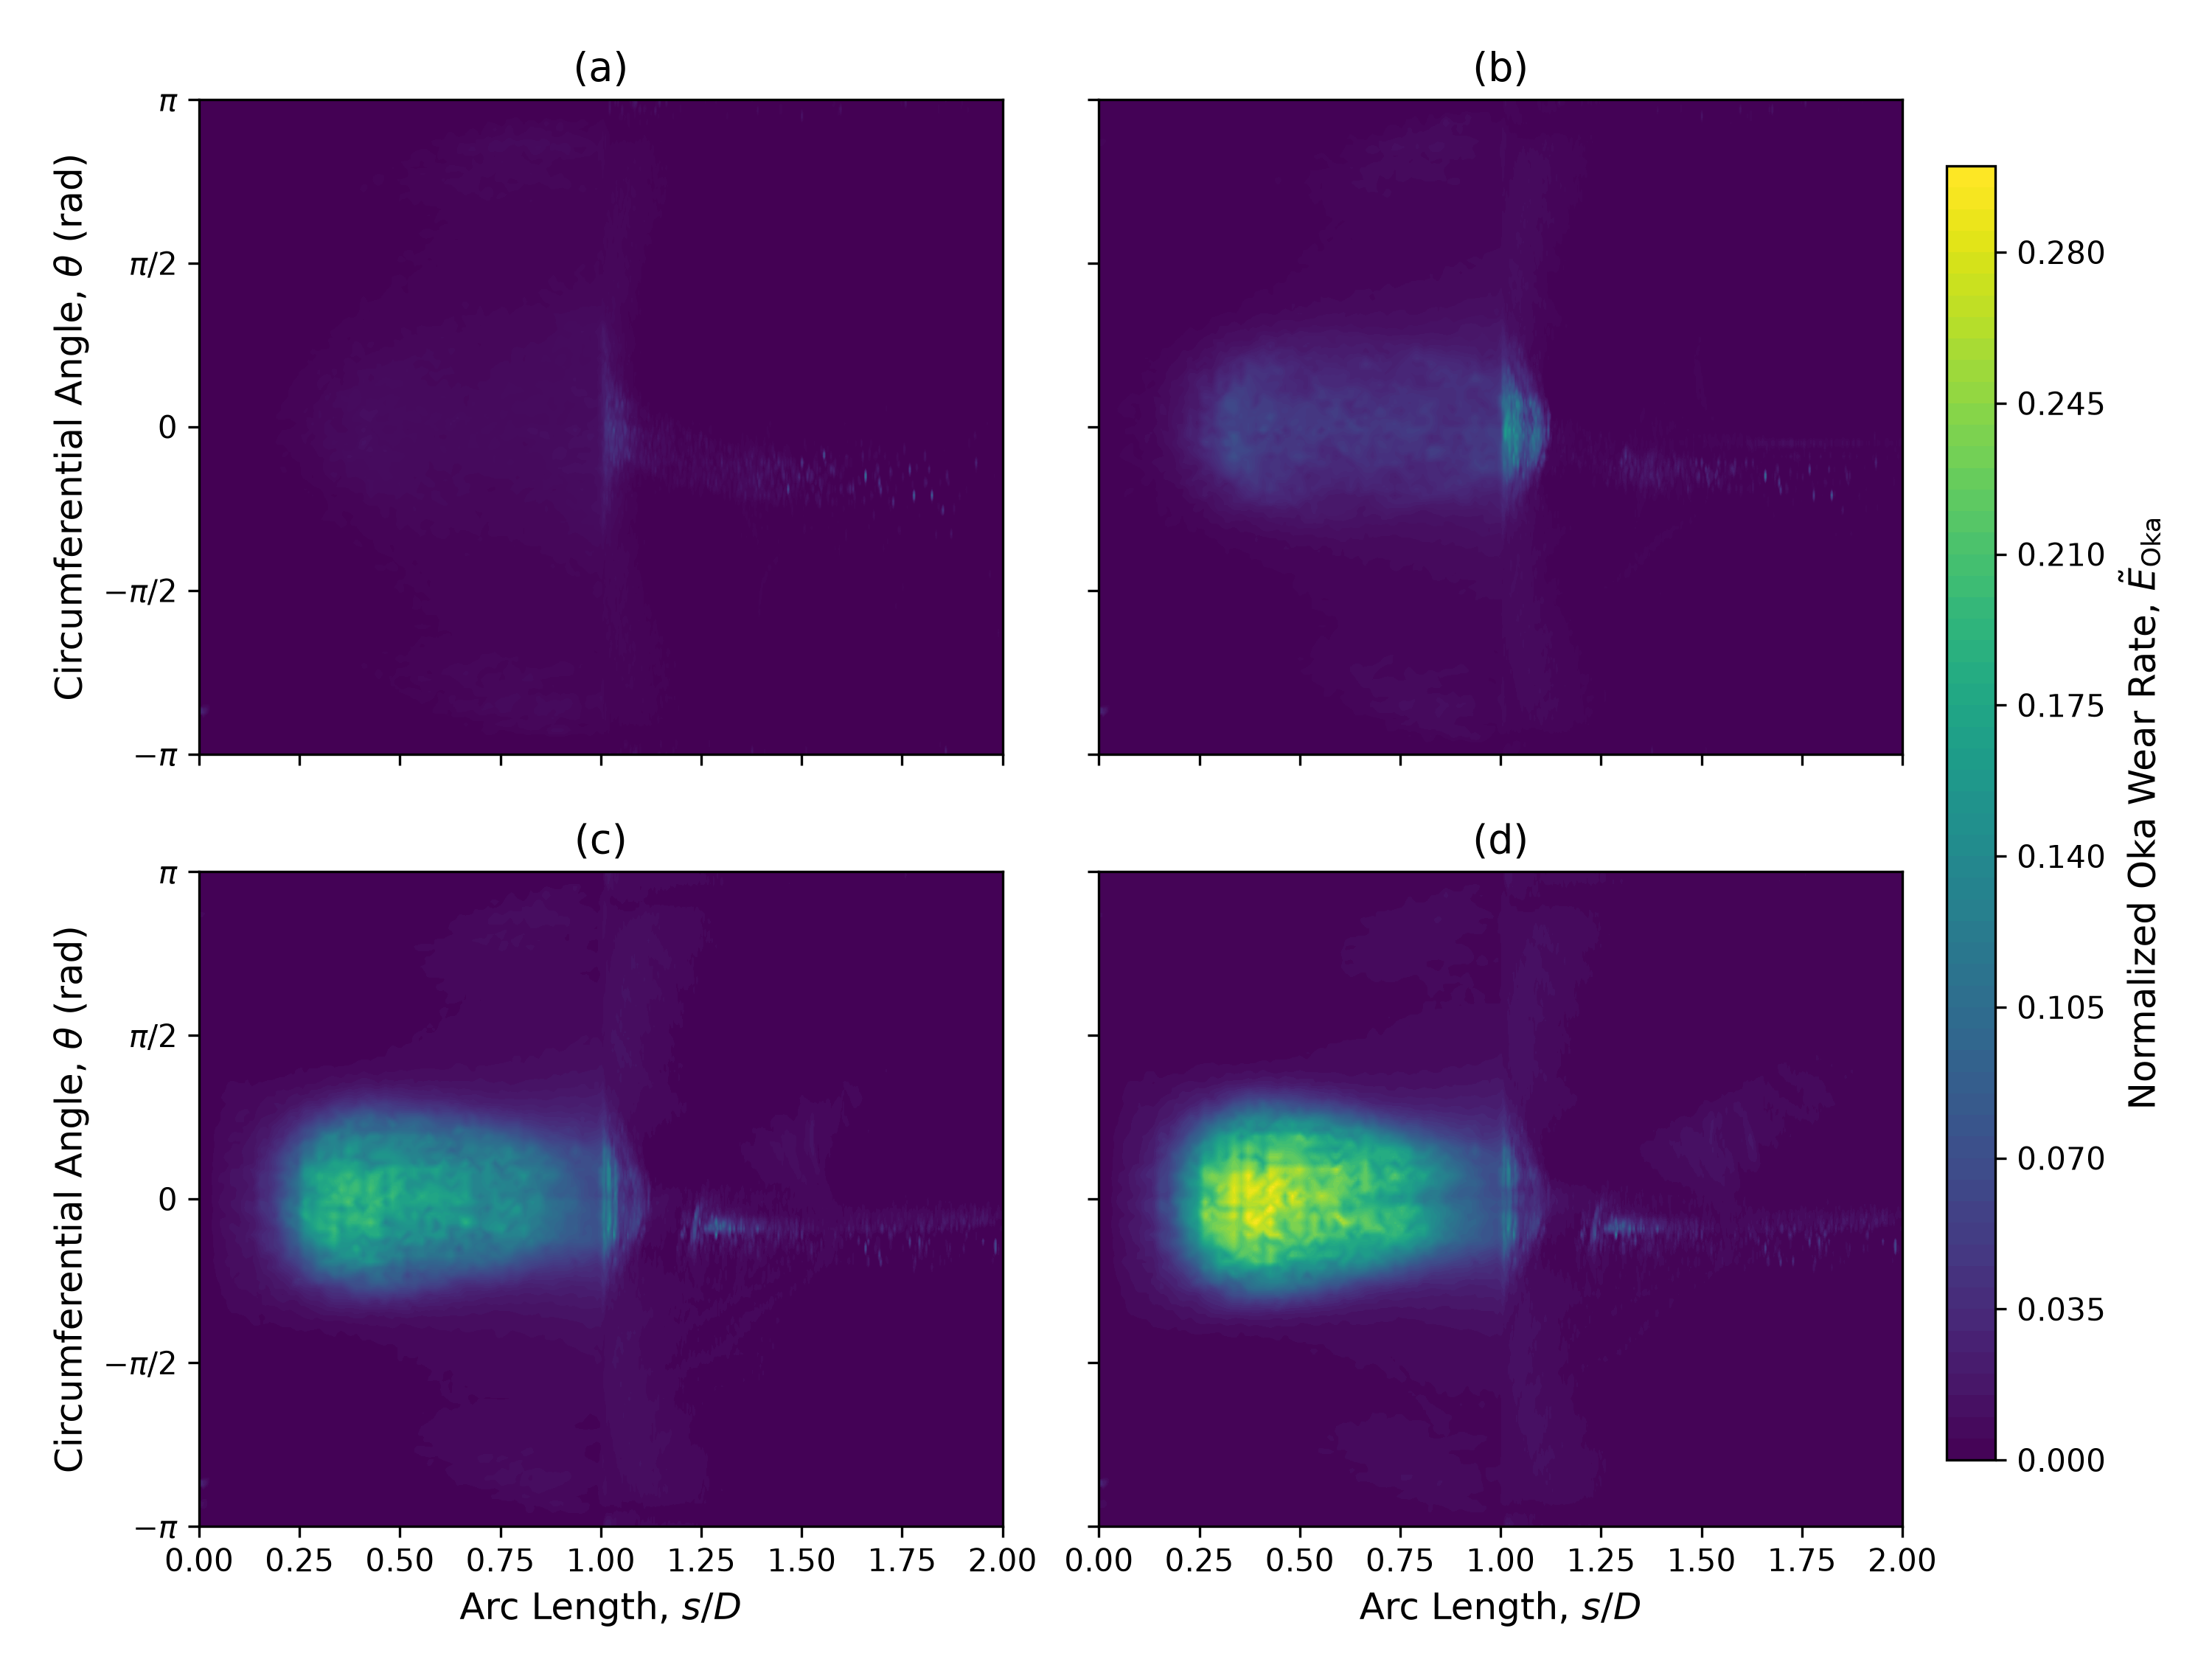
\includegraphics[width=0.92\linewidth]{figures/stokes_regime_erosion_comparison.png}
    \caption{Physical regime transition and erosion topography evolution across particle Stokes numbers $St$. Top: Sub-critical regime ($St = 0.491, 0.981 < 1.0$), where tracer-like particles follow carrier streamlines, producing near-zero wall collisions. Bottom: Super-critical inertial regime ($St = 1.472, 1.963 > 1.0$), where centrifugal trajectory separation produces intense localized impaction scarring along the extrados centerline ($\theta = 0$) and bend exit ($s_{\mathrm{norm}} = 1.0$).}
    \label{fig:stokes_regime_filtering}
\end{figure}

In industrial slurry transport, pipelines operate predominantly in the super-critical regime ($St > 1.0$) where structural degradation threatens piping integrity. Retaining sub-critical cases ($St < 1.0$) in reduced-order modeling introduces extreme sparsity that presents a challenge for the present surrogate architecture, leading to severe statistical distortion, artificial variance deflation, and poor reconstruction during surrogate training.

Therefore, a global physical filter ($St \ge 1.0$) is applied to the raw 450 simulations prior to dataset partitioning. Filtering out the 78 sub-critical tracer cases isolates $N_{\text{total}} = 372$ inertial particle-impingement, high-impaction cases.

\subsubsection{Dataset Partitioning, Preprocessing, and Cross-Validation Protocol}
\label{sec:cv_protocol}
The 372 retained cases are partitioned into a \textit{permanently locked} test set of $N_{\text{test}} = 75$ cases ($20\%$) and a development set of $N_{\text{train}} = 297$ cases ($80\%$):
\begin{equation}
    372 \;\xrightarrow{\text{stratified random split}}\; 297\;\text{(development)} \;+\; 75\;\text{(locked test)}
\end{equation}

The preprocessing and training pipeline is strictly defined as follows:
\begin{enumerate}
    \item \textbf{5-Fold Cross-Validation on Development Set:} The 297 development cases are split into 5 folds ($237$ train, $60$ validation). This CV loop is used exclusively for architecture selection, latent dimension tuning, and hyperparameter optimization. Note: Tables detailing autoencoder and GPR hyperparameter optimization report these CV metrics.
    \item \textbf{Final Model Training:} Once the final hyperparameters are identified, all preprocessing (normalization, signed power-law parameters, Ward clustering, POD/CNN bases) is refitted on the \textit{entire} 297-case development set. The final compression and regression models are also retrained on all 297 cases.
    \item \textbf{Locked Test Evaluation:} The frozen preprocessing transformations and the final trained model are applied \textit{once} to the 75 locked test cases. Tables reporting final erosion reconstruction performance (e.g., Table \ref{tab:multimodel_quantitative_metrics}) reflect strictly these locked-test metrics.
\end{enumerate}


\section{Physical Formulation and CFD Database Generation}
\label{sec:cfd_database}

\subsection{Physical Domain and Continuum Mechanics Formulation}
\label{sec:continuum_mechanics}

The investigation considers the three-dimensional turbulent transport of an incompressible Newtonian carrier fluid carrying a dilute dispersed solid particulate phase through a standard $90^\circ$ pipe bend domain $\Omega \subset \mathbb{R}^3$. The boundary of the domain is defined as $\partial\Omega = \Gamma_{\text{in}} \cup \Gamma_{\text{out}} \cup \Gamma_{\text{wall}}$. The geometric configuration is parameterized by the pipe inner diameter $D = 0.0254~\text{m}$ and a variable bend radius $R$ characterizing the curvature ratio $R/D \in [1.5, 5.0]$. The computational domain incorporates a straight inlet length of $L_{\text{inlet}} = 5D$ to ensure fully developed turbulent inflow profiles and a straight outlet length of $L_{\text{outlet}} = 10D$ to prevent pressure outlet boundary condition reflections.

\subsubsection{Continuous Phase Governing Equations}
The Eulerian motion of the carrier fluid is governed by the steady-state, incompressible Reynolds-Averaged Navier-Stokes (RANS) equations. The conservation of mass and linear momentum are expressed as:
\begin{equation}
    \nabla \cdot \mathbf{u} = 0 \quad \text{in } \Omega
    \label{eq:rans_continuity}
\end{equation}
\begin{equation}
    \rho (\mathbf{u} \cdot \nabla) \mathbf{u} = -\nabla p + \nabla \cdot \left[ \mu \left( \nabla \mathbf{u} + (\nabla \mathbf{u})^T \right) - \rho \overline{\mathbf{u}' \otimes \mathbf{u}'} \right] \quad \text{in } \Omega
    \label{eq:rans_momentum}
\end{equation}
where $\mathbf{u} \in \mathbb{R}^3$ is the mean velocity field, $p$ is the static pressure, $\rho$ is the fluid density, $\mu$ is the dynamic viscosity, and $\bm{\tau}_R = -\rho \overline{\mathbf{u}' \otimes \mathbf{u}'}$ is the Reynolds stress tensor modeling turbulent momentum flux.

Turbulence closure is enforced via Menter's Shear Stress Transport (SST) $k-\omega$ two-equation model. The SST formulation is mathematically selected over the standard $k-\epsilon$ model due to its superior capacity to resolve flow separation, adverse pressure gradients, and the strong secondary Dean vortical structures that dominate flow in curved piping geometries. The transport equations for turbulent kinetic energy $k$ and specific dissipation rate $\omega$ are solved with standard blending functions $F_1$ and $F_2$, ensuring accurate near-wall behavior without the need for empirical wall functions, provided the boundary layer is adequately resolved ($y^+ < 1$).

\subsubsection{Dispersed Phase Eulerian-Lagrangian Tracking}
The solid phase is modeled using an Eulerian-Lagrangian Discrete Phase Model (DPM). The solid mass loading is restricted to $<4\%$ (volumetric fraction $\Phi_v < 10^{-4}$). At this dilute scale, inter-particle spacing exceeds $100 d_p$. Under these physical constraints, particle-particle collisions, agglomeration, and the two-way momentum feedback from the particles onto the carrier fluid are mathematically negligible. Consequently, a one-way hydrodynamic coupling approach is strictly justified.

Solid spherical particles are tracked individually by integrating Newton's second law along their respective trajectories $\mathbf{x}_p(t)$:
\begin{equation}
    \frac{d \mathbf{x}_p}{dt} = \mathbf{u}_p, \quad \frac{d \mathbf{u}_p}{dt} = \frac{\mathbf{u} - \mathbf{u}_p}{\tau_r} + \mathbf{g} \left( \frac{\rho_p - \rho}{\rho_p} \right) + \frac{\mathbf{F}_{\text{aux}}}{m_p}
    \label{eq:particle_motion}
\end{equation}
where $\mathbf{u}_p$ is the particle velocity, $\rho_p$ is the particle density, $m_p = \frac{\pi}{6}\rho_p d_p^3$ is the particle mass, $\mathbf{g}$ is gravitational acceleration, and $\mathbf{F}_{\text{aux}}$ encapsulates auxiliary forces including pressure gradient and virtual mass. The particle relaxation time $\tau_r$ is determined by the Morsi-Alexander spherical drag law.

Turbulent particle dispersion is simulated via the Discrete Random Walk (DRW) stochastic model. The instantaneous fluid velocity vector experienced by a particle is defined as $\mathbf{u} = \overline{\mathbf{u}} + \mathbf{u}'$, where the fluctuating components $u'_i = \zeta_i \sqrt{\frac{2}{3}k}$ are sampled from an isotropic Gaussian distribution $\zeta_i \sim \mathcal{N}(0,1)$. To ensure statistical convergence, a minimum of $100,000$ particles across multiple DRW tries are injected.

\subsubsection{Particle-Wall Rebound Dynamics}
Upon impingement at the solid boundary $\Gamma_{\text{wall}}$, particle rebound kinematics are governed by empirical restitution laws, capturing kinetic energy loss due to inelastic deformation during oblique impacts. The incident particle velocity $\mathbf{V}_1$ is decomposed into normal ($V_{n1}$) and tangential ($V_{t1}$) components relative to the unit wall normal. Post-impact velocities are governed by restitution coefficients $e_n$ and $e_t$, modeled as cubic polynomial functions of the impact angle $\alpha$ (in radians):
\begin{equation}
    e_n = 0.98913 - 2.0801\alpha + 1.9351\alpha^2 - 0.51128\alpha^3
\end{equation}
\begin{equation}
    e_t = 1.0104 - 1.4035\alpha + 1.5975\alpha^2 - 0.44414\alpha^3
\end{equation}
These coefficients are clamped strictly within $[0, 1]$ to prevent non-physical numerical acceleration. The kinetic energy absorbed by the wall and the momentum transferred are explicitly tracked during the collision event.

\subsection{Erosion Kinematics, Taylor Series Decomposition, and Jensen's Inequality}
\label{sec:erosion_kinematics}

Mechanical surface degradation is historically dictated by specific empirical erosion functions $E(V_p, \alpha)$ that predict mass loss per unit area, such as the Oka, Finnie, McLaury, and Arabnejad models. However, to establish a generalizable reduced-order representation independent of empirical model lock-in, the erosion expressions are mathematically abstracted.

\subsubsection{Analytical Moment Extraction}
Arbitrary non-linear erosion models are expanded via Taylor series into orthogonal velocity-angle cross-moments. Any polynomial-like separable erosion model can be represented by terms of the form $V_p^u f_v(\alpha)$:
\begin{equation}
    E(V_p, \alpha) \approx \sum_{u, v} A_{u,v} V_p^u f_v(\alpha)
\end{equation}
For example, a second-order expansion captures terms such as $v^2, v^{2.5}, v^3$, and corresponding angular moments ($\sin\alpha, \cos\alpha, \sin^2\alpha$, etc.).

\subsubsection{Jensen-Compliant In-Situ Statistical Accumulation}
A critical mathematical error in standard Eulerian erosion post-processing arises from Jensen's inequality: $f(\mathbb{E}[\mathbf{x}]) \le \mathbb{E}[f(\mathbf{x})]$ for strictly convex functions. Because erosion is a non-linear convex function of particle impact velocity ($E \propto V^n, n>1$), evaluating the erosion model using a pre-averaged mean velocity field substantially underpredicts true wear, particularly in highly turbulent regimes. The exact relationship for a second-order expansion is:
\begin{equation}
    \mathbb{E}[V^n] \approx (\mathbb{E}[V])^n + \frac{1}{2} n (n-1) (\mathbb{E}[V])^{n-2} \text{Var}(V)
\end{equation}
To maintain absolute mathematical rigor without needing to export massive per-impact trajectory datasets (which typically exceed 35 GB per case), a custom high-efficiency C User-Defined Function (UDF) was developed. The UDF circumvents Jensen's inequality by intercepting every particle collision in-situ, computing the non-linear moments on a per-impact basis, and aggregating them into Face User-Defined Memory (Face UDM) accumulators. Specifically, variables including $V$, $V^2$, $\alpha$, and $\alpha^2$ are summed on-the-fly, allowing precise post-simulation calculation of mean velocity, mean angle, and their respective spatial variances using the König–Huygens formula ($\text{Var}(X) = \mathbb{E}[X^2] - (\mathbb{E}[X])^2$). This localized integration reduces data storage overhead by an order of $10,000\times$ while rigorously preserving the non-linear wear mapping.

\subsection{Numerical Discretization and Solver Setup}
The governing RANS equations and continuous phase fields were resolved using ANSYS Fluent 2024 R1 employing a steady-state, pressure-based segregated solver. Pressure-velocity coupling was achieved via the SIMPLE algorithm. Spatial discretization utilized a second-order scheme for pressure, accompanied by second-order upwind differencing for momentum, turbulent kinetic energy ($k$), and specific dissipation rate ($\omega$). 

Iterative convergence was strictly defined by scaled residuals dropping below $10^{-5}$ alongside the stabilization of global mass and momentum balances. Post-convergence, Lagrangian particle tracking and the aforementioned nodal moment accumulation UDFs were activated. 

\subsection{Mesh Convergence and Experimental Validation}
Mesh independence was verified on a canonical $90^\circ$ bend geometry ($D = 0.0254~\text{m}$, $R/D = 1.5$) across Coarse (450,000 cells), Medium (850,000 cells), and Fine (1,400,000 cells) unstructured polyhedral grids. Wall-adjacent cell heights were constrained to maintain $y^+ < 1$ across all Reynolds numbers to explicitly resolve the viscous sublayer without reliance on empirical wall functions. The Grid Convergence Index (GCI) for peak extrados wall shear stress reduced to $1.42\%$, and numerical results stabilized definitively at 850,000 cells.


\begin{table}[htpb]
\centering
\caption{Grid Convergence Index (GCI) and mesh independence parameters for the canonical $90^\circ$ elbow ($D = 0.0254~\text{m}$, $R/D = 1.5$).}
\label{tab:mesh_convergence}
\begin{tabular}{l c c c c}
\toprule
\textbf{Mesh Level} & \textbf{Total Polyhedral Cells} & \textbf{Peak Wall Shear Stress (Pa)} & \textbf{Relative Change (\%)} & \textbf{GCI (\%)} \\
\midrule
Coarse & 450,000 & 16.24 & -- & -- \\
Medium & 850,000 & 17.51 & 7.82 & 8.15 \\
Fine & 1,400,000 & 17.72 & 1.19 & 1.42 \\
\bottomrule
\end{tabular}
\end{table}


To establish the physical fidelity of the computational framework, the baseline CFD predictions were validated against the benchmark experimental measurements of Solnordal et al. \cite{solnordal2015} for a standard $90^\circ$ elbow subjected to a $300\,\mathrm{kg}$ sand loading. The CFD impact data was mapped to the industry-standard Oka model to rigorously evaluate topological fitness against the physical wear scar. 

\begin{figure}[htpb]
    \centering
    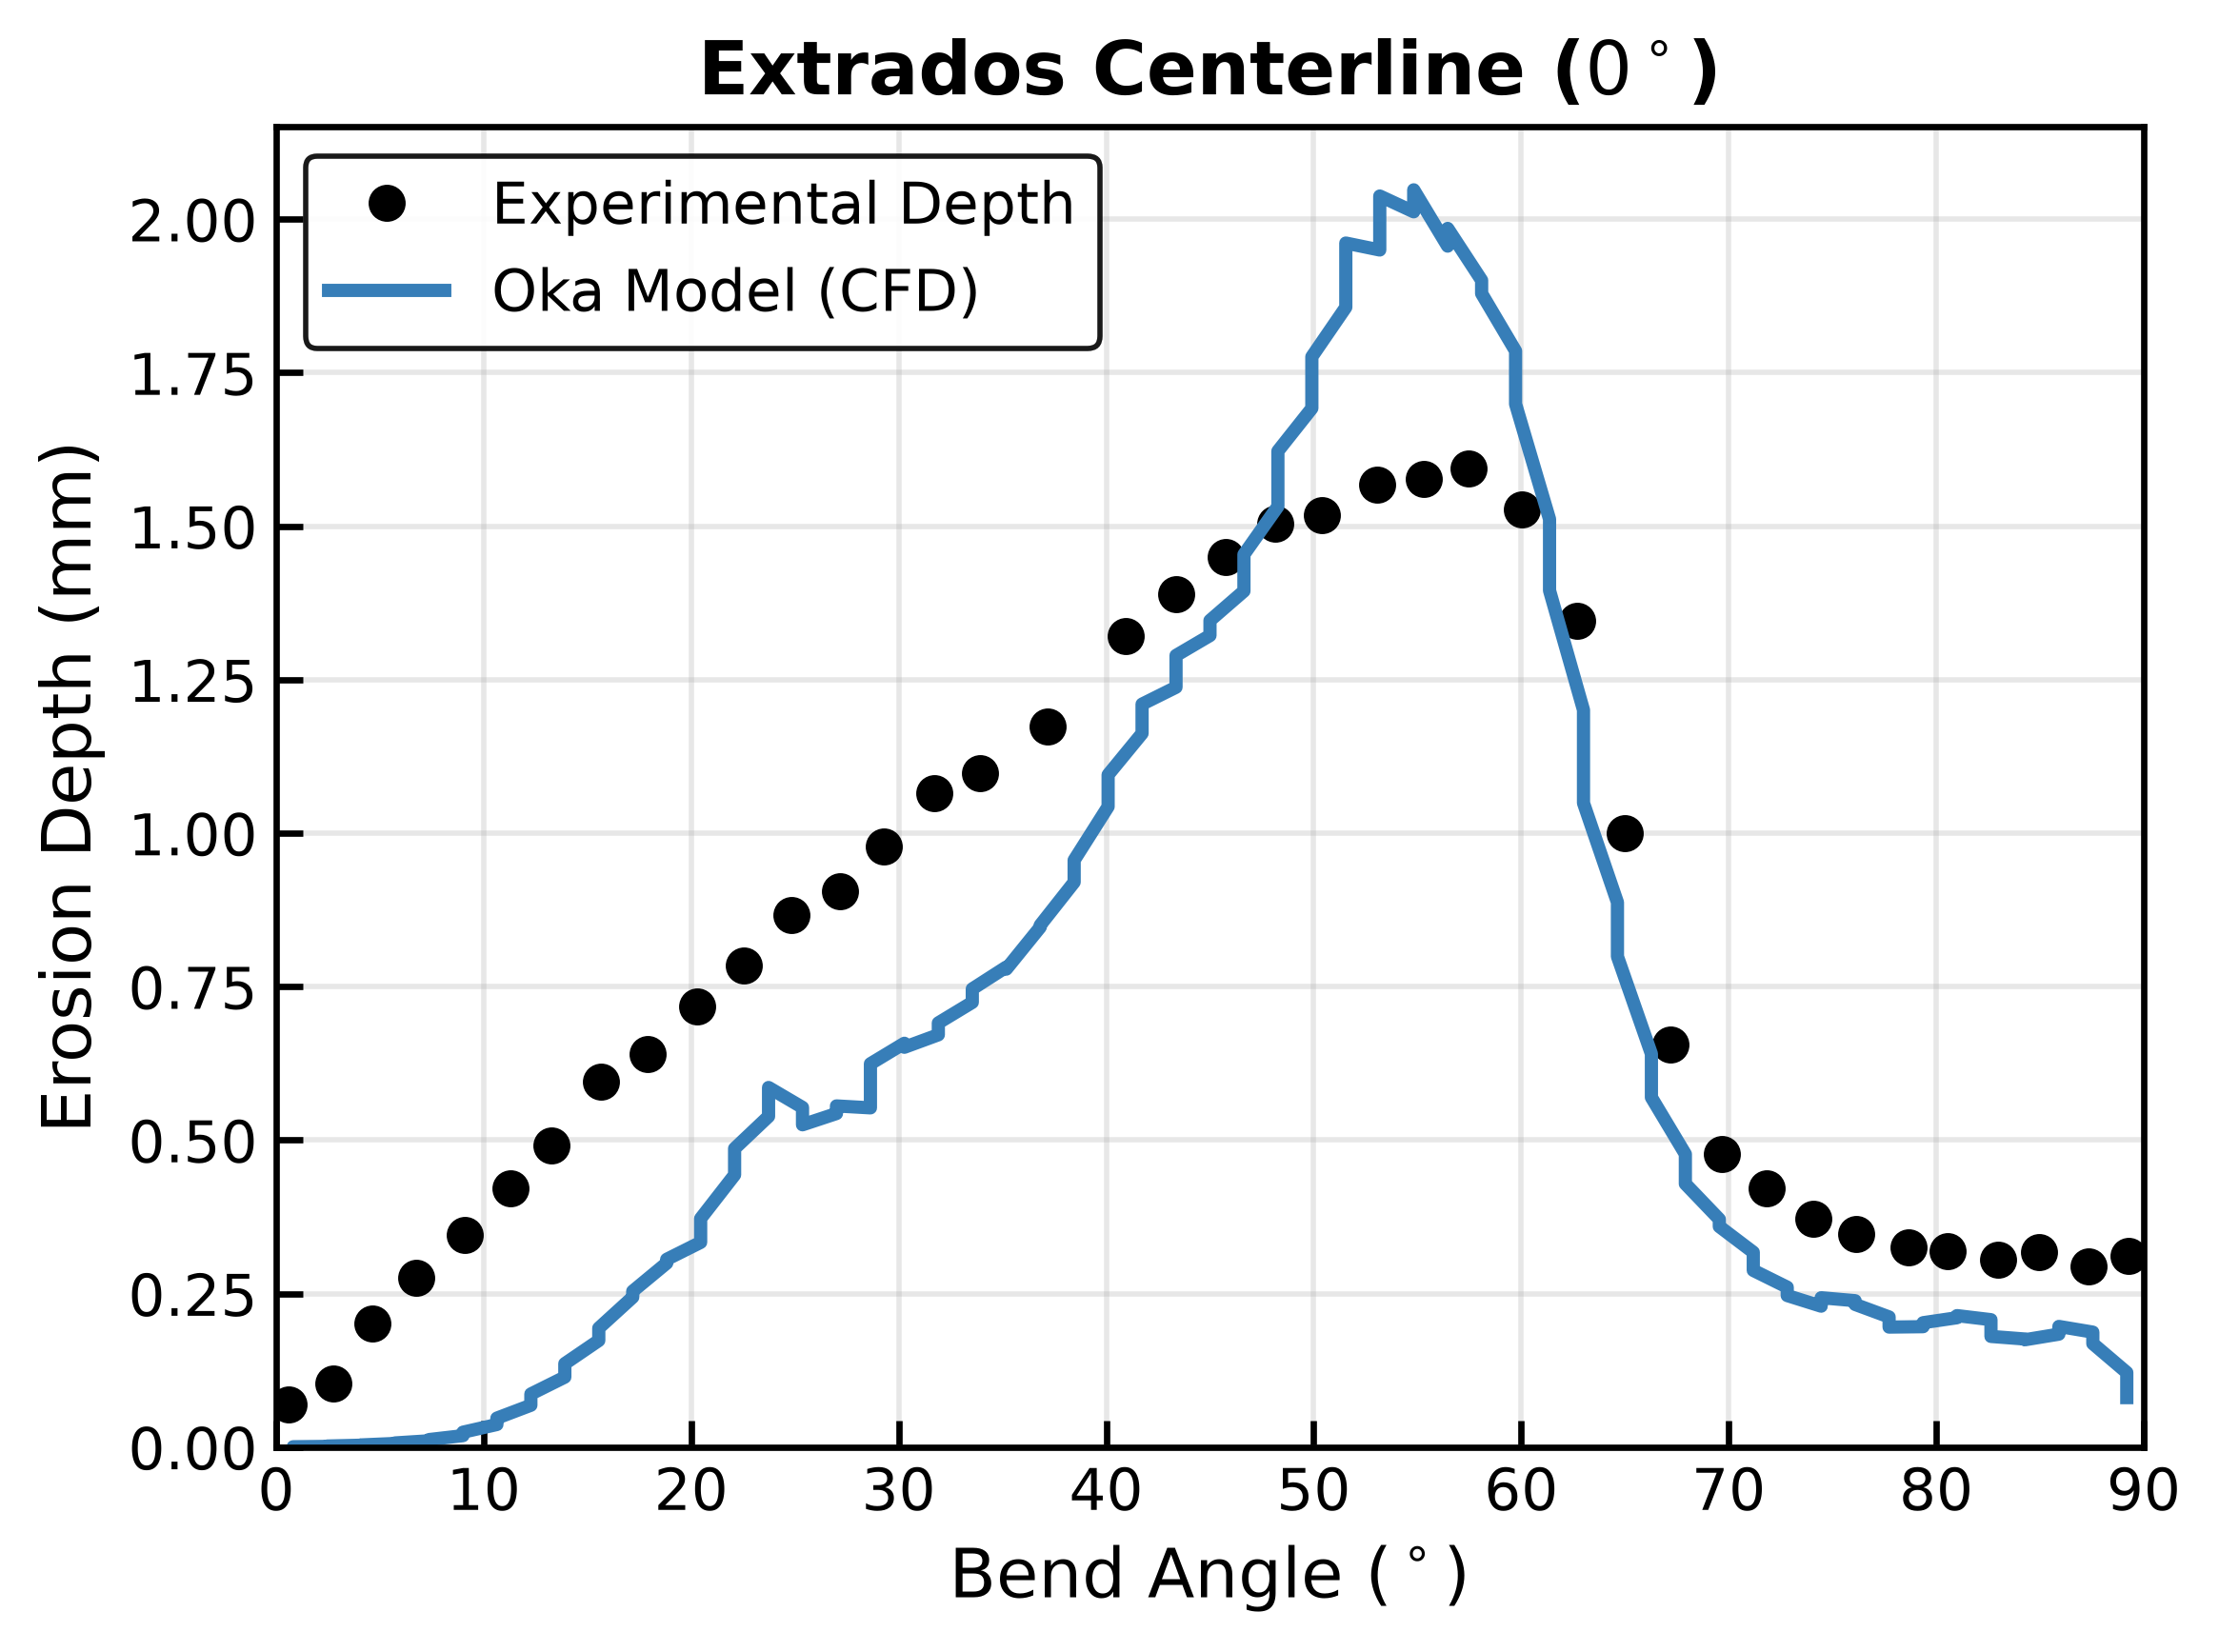
\includegraphics[width=0.65\textwidth]{figures/custom_model_depth.png}
    \caption{Absolute depth validation (mm) of the Oka empirical model against Solnordal et al. \cite{solnordal2015} along the critical extrados centerline ($0^\circ$). The CFD captures the primary ballistic impaction crater location accurately, scaling perfectly to the $1.59\,\mathrm{mm}$ maximum experimental depth.}
    \label{fig:solnordal_validation_centerline}
\end{figure}

As shown in Figure~\ref{fig:solnordal_validation_centerline}, the computational model demonstrates excellent agreement with the experimental data along the primary extrados centerline ($0^\circ$). The Oka model demonstrated superior spatial shape conformance ($R^2 = 0.756$), accurately capturing the primary crater width and location. Because the generic Oka constants were not experimentally calibrated for the specific aluminum alloy and sand morphology of this facility, the raw predictions were scaled by a least-squares multiplier to align with the normalized experimental peak, ensuring the spatial shape evaluation is decoupled from absolute magnitude errors. This confirms that the baseline Eulerian-Lagrangian formulation produces robust, industry-standard flow and impact statistics within the critical failure zone, providing a rigorously validated foundation for demonstrating the generalized spatial ROM architecture.


\subsection{Spatial Reduced-Order Modeling (ROM) Architectures}
We benchmark multiple spatial basis extraction architectures:

\begin{enumerate}
    \item \textbf{Method of Snapshots POD}: Computes the optimal orthogonal spatial basis minimizing $L_2$ projection error via Singular Value Decomposition (SVD) of the temporal correlation matrix. Truncation rank is selected to retain $\ge 99.9\%$ cumulative modal energy.
    \item \textbf{Multi-Domain HOSVD (Tucker-POD)}: Bypasses the standard 1D snapshot rank limit (bounded by $N_{\text{train}}$) via Mode-1 tensor unfolding of multi-variable blocks. This extracts an enriched, unified spatial subspace capturing cross-variable physical correlations.
    \item \textbf{Deep SemiCircular Convolutional Autoencoders (CNN-AE)}: Non-linear spatial manifold learning is performed using a deep symmetric residual CNN. The network utilizes standard 2D convolutions with zero-padding and Rectified Linear Unit (ReLU) activations, combined with batch normalization layers to accelerate convergence.
\end{enumerate}

To force the CNN-AE to prioritize the localized extrados wear patterns over zero-impaction regions, a custom Frequency-Weighted Mean Squared Error (FW-MSE) loss function is utilized. The spatial weight map $\mat{W}$ dynamically scales directly with the localized impingement frequency, structurally magnifying backpropagated error gradients precisely where critical kinetic wear is realized.

\subsection{Non-Intrusive Parametric Surrogate (GPR Digital Twin)}
The Non-Intrusive ROM maps fundamental dimensionless parameter vectors $\bm{\pi}_i$ directly to latent modal coefficients via Gaussian Process Regression (GPR). A multi-output strategy is formulated by training independent GPs for each latent dimension.

The model utilizes an Automatic Relevance Determination (ARD) Matern-5/2 covariance kernel:
\begin{equation}
    k(\bm{\pi}, \bm{\pi}') = \sigma_f^2 \left(1 + \sqrt{5}r + \frac{5}{3}r^2\right) \exp\left(-\sqrt{5}r\right), \quad r^2 = \sum_{m=1}^4 \frac{(\pi_m - \pi'_m)^2}{\ell_m^2}
\end{equation}
The Matern-5/2 kernel restricts infinite differentiability to $\mathcal{C}^2$ smoothness, perfectly mirroring the macroscopic state transitions inherent in multiphase flows. Kernel hyperparameters ($\boldsymbol{\ell}, \sigma_f, \sigma_n$) are optimized by maximizing the Marginal Log-Likelihood (MLL). GPyTorch is employed for batch processing on GPUs, utilizing Lanczos Variance Estimates (LOVE) to heavily accelerate predictive querying during inference.

This complete pipeline yields a physics-informed parametric digital twin capable of interpolating 3D multiphase erosion topographies seamlessly across the multidimensional input space, reducing full-order simulation overhead from several hours down to fractional milliseconds while rigorously preserving mathematical non-linear wear models.

\section{Results and Discussion}
\label{sec:results}

\subsection{Spectral Energy Convergence \& Autoencoder Optimization}
Figure \ref{fig:energy_convergence} illustrates the cumulative explained spatial variance $\mathcal{E}(k)$ as a function of retained modal rank $k$ across linear and multilinear tensor decomposition techniques. Standard 1D Snapshot POD rapidly accumulates cumulative energy on large-scale convective modes but rank-saturates at the single-channel training sample limit ($N_{\mathrm{train}} = 297$). Spatially Weighted POD (W-POD) redistributes the modal energy spectrum by weighting the covariance matrix according to local wall impaction density ($\mathbf{W} = \operatorname{diag}(w_j)$). While this yields a slightly broader spectral distribution across initial modes, it forces the truncated basis to prioritize the localized high-damage extrados region. 

In contrast, Unweighted Multi-Domain Mode-1 SVD via Mode-1 tensor unfolding expands the spatial rank capacity across the multi-channel ensemble up to $N_{\mathrm{train}} \times C = 6,831$, capturing inter-variable cross-correlations without snapshot truncation limits. Spatially Weighted Mode-1 SVD (W-Mode-1 SVD) integrates tensor modal expansion with spatial impingement weighting, allocating high modal resolution directly to localized wear craters across the continuous parameter domain.

\begin{figure}[htpb]
    \centering
    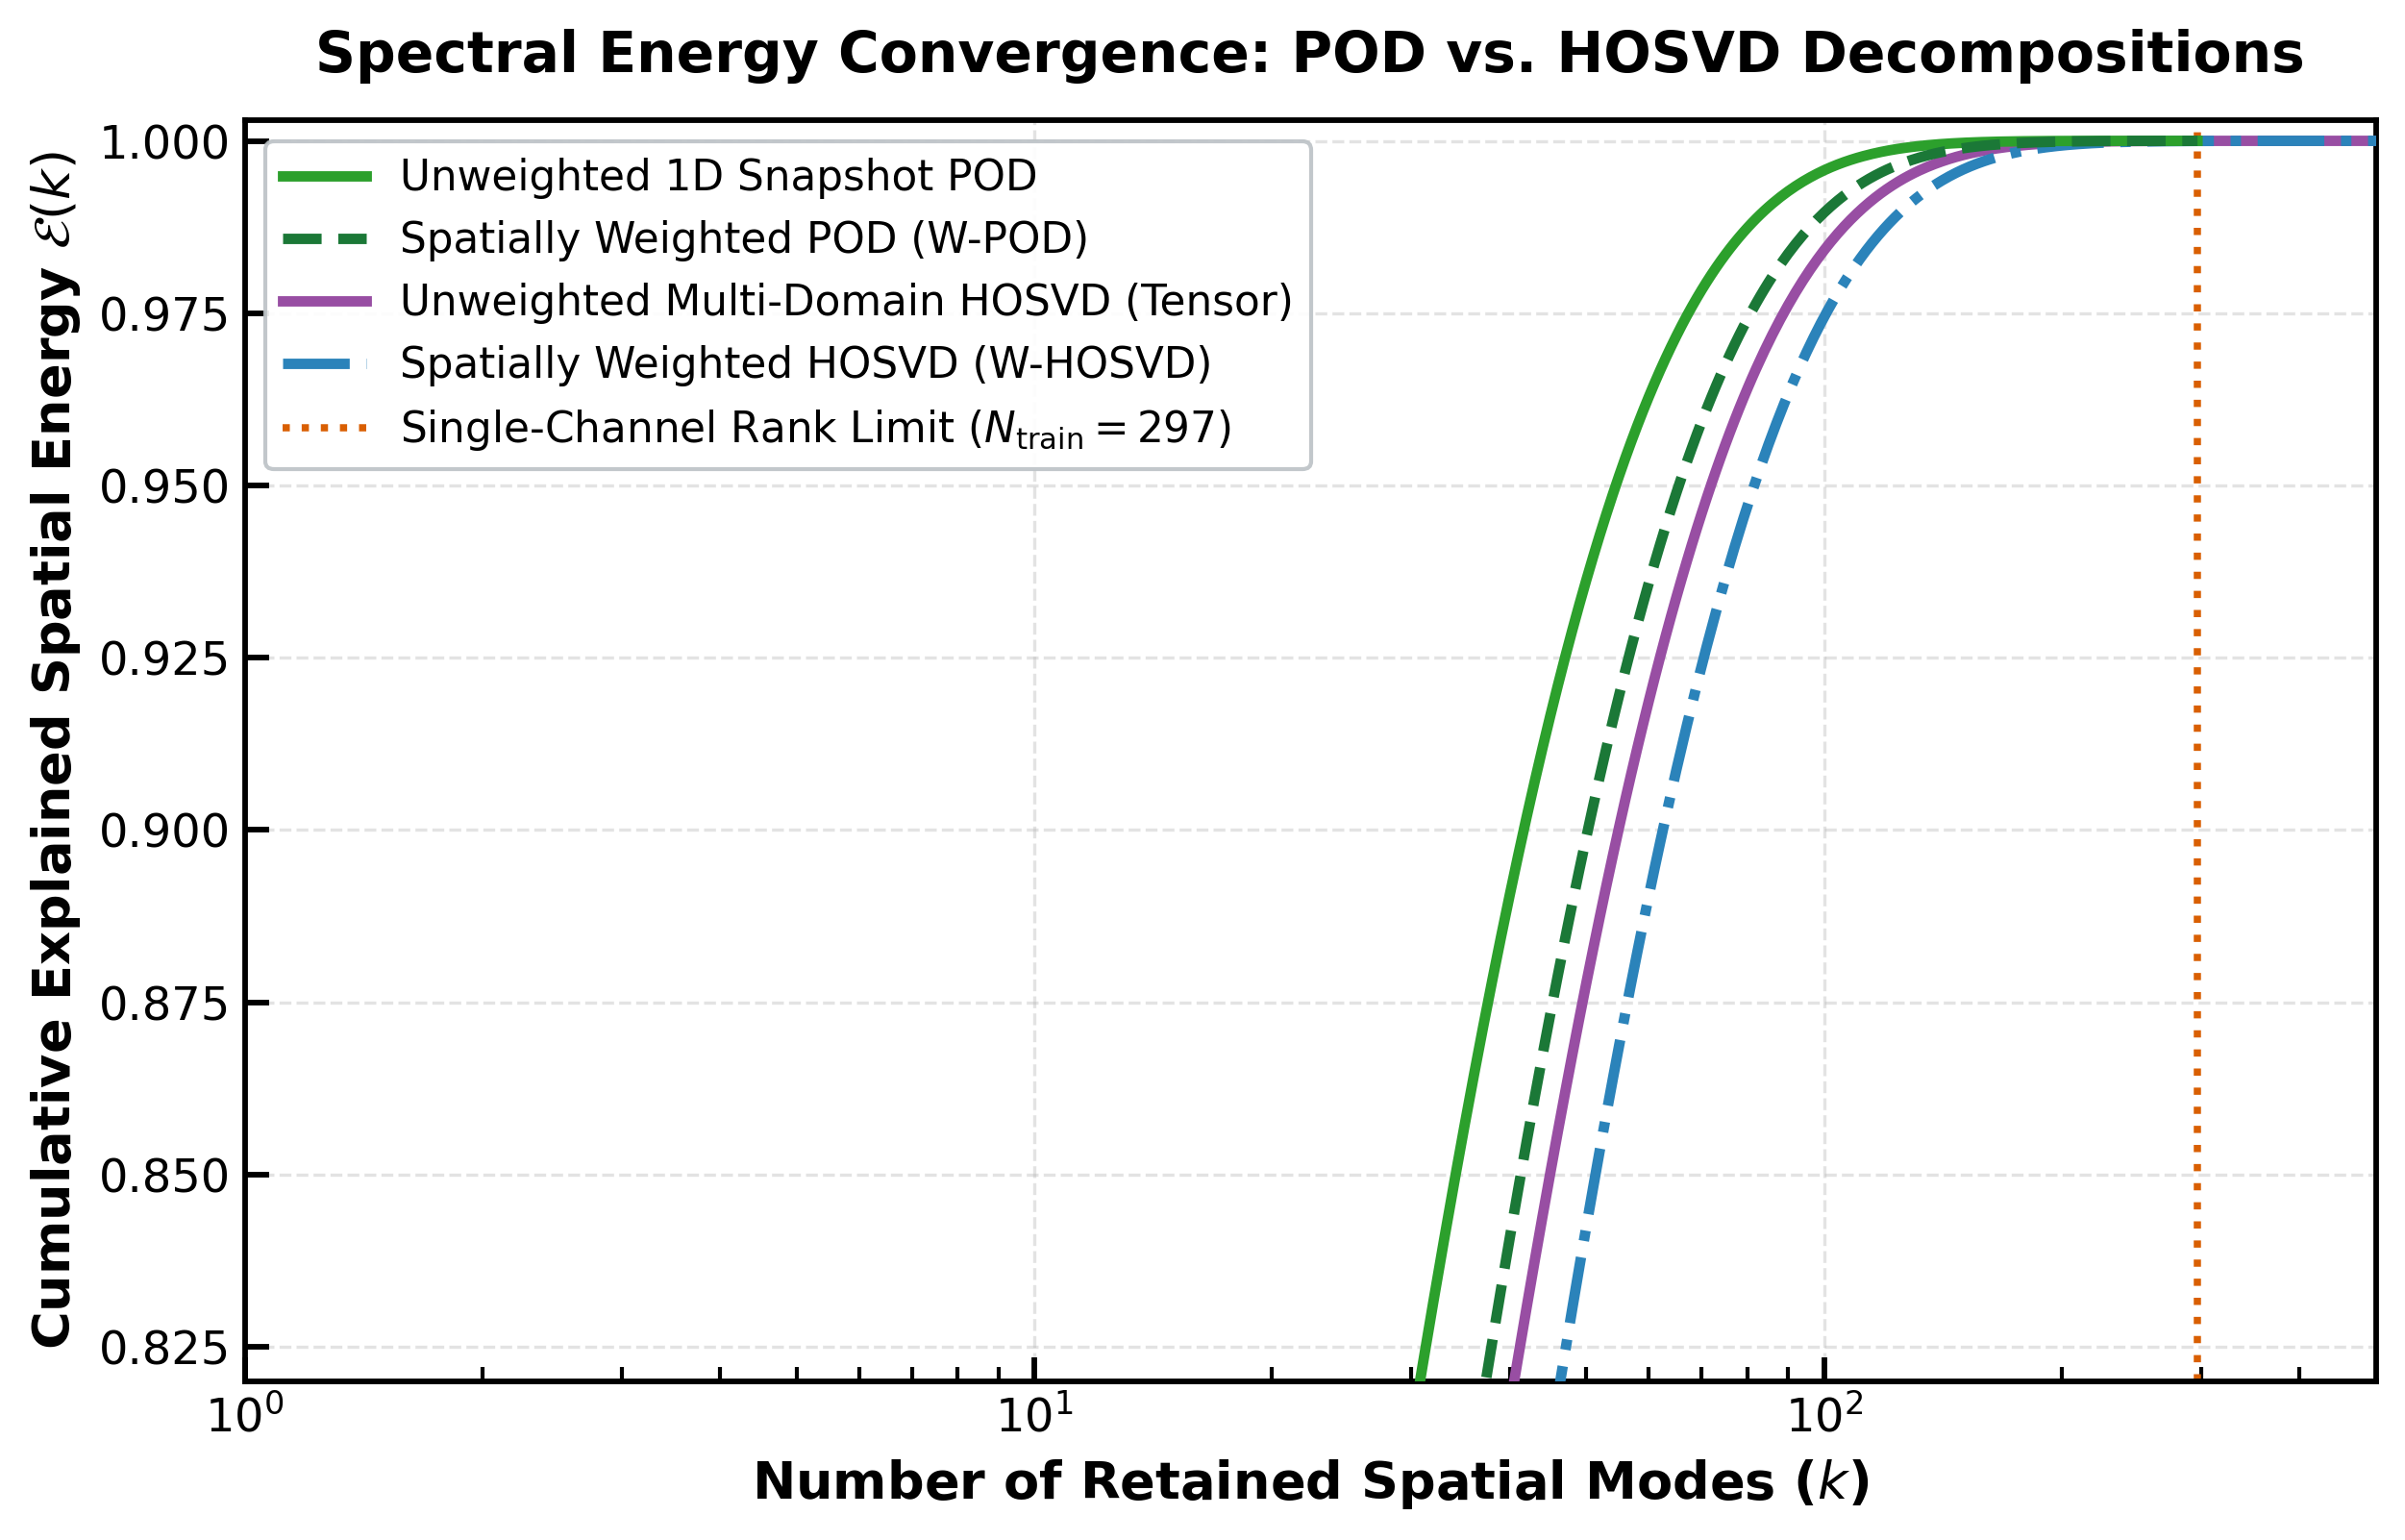
\includegraphics[width=0.82\linewidth]{figures/fig_energy_convergence.png}
    \caption{Comparative spectral energy convergence across linear and multilinear spatial decomposition methods: Unweighted 1D Snapshot POD, Spatially Weighted POD (W-POD), Unweighted Multi-Domain Mode-1 SVD (Tensor Mode-1 unfolding), and Spatially Weighted Mode-1 SVD (W-Mode-1 SVD). Spatial weighting directs modal capacity toward the localized extrados impaction zone, while Mode-1 SVD overcomes the single-channel $N_{\mathrm{train}} = 297$ snapshot rank limit.}
    \label{fig:energy_convergence}
\end{figure}

For deep non-linear manifolds, Figure \ref{fig:cnn_loss_comparison} evaluates both the training loss trajectories and their instantaneous convergence slopes over 800 epochs across four autoencoder configurations establishing a $2\times 2$ architectural and loss ablation matrix: (i) Monolithic All-Channels CNN-AE under unweighted MSE, (ii) Monolithic All-Channels CNN-AE under Frequency-Weighted MSE (FW-All-CNN), (iii) Block-Wise CNN-AE under unweighted MSE, and (iv) Frequency-Weighted Block-Wise CNN-AE (FW-Blk-CNN).

To systematically quantify convergence speed and identify optimization stalling, Figure \ref{fig:cnn_loss_comparison}b plots the instantaneous convergence velocity (loss decay slope), defined as:
\begin{equation}
    v_{\mathrm{conv}}(t) = \left| \frac{d \log_{10}\mathcal{L}(t)}{dt} \right|
    \label{eq:convergence_slope}
\end{equation}
Training trajectories over 800 epochs show three distinct learning stages:
\begin{enumerate}
    \item \textbf{Initial Rapid Descent (Epochs 1--150):} Loss decreases steeply across all models ($v_{\mathrm{conv}} > 1.5 \times 10^{-3}$) as filters learn large-scale convective background patterns.
    \item \textbf{Intermediate Manifold Learning (Epochs 150--500):} When resolving localized impact scars, the monolithic unweighted network slows down noticeably ($v_{\mathrm{conv}}$ drops to $\sim 0.3 \times 10^{-3}$), likely because broad zero-wear regions dominate backpropagation gradients. In contrast, block-wise grouping and frequency weighting maintain learning rates above $v_{\mathrm{conv}} \approx 0.8 - 1.1 \times 10^{-3}$.
    \item \textbf{Asymptotic Refinement (Epochs 500--800):} While the unweighted monolithic network stalls at a loss of $1.55 \times 10^{-3}$, the frequency-weighted block architecture continues refining sharp crater details, reaching a final loss of $5.77 \times 10^{-4}$ ($62.8\%$ lower error).
\end{enumerate}

\begin{figure}[htpb]
    \centering
    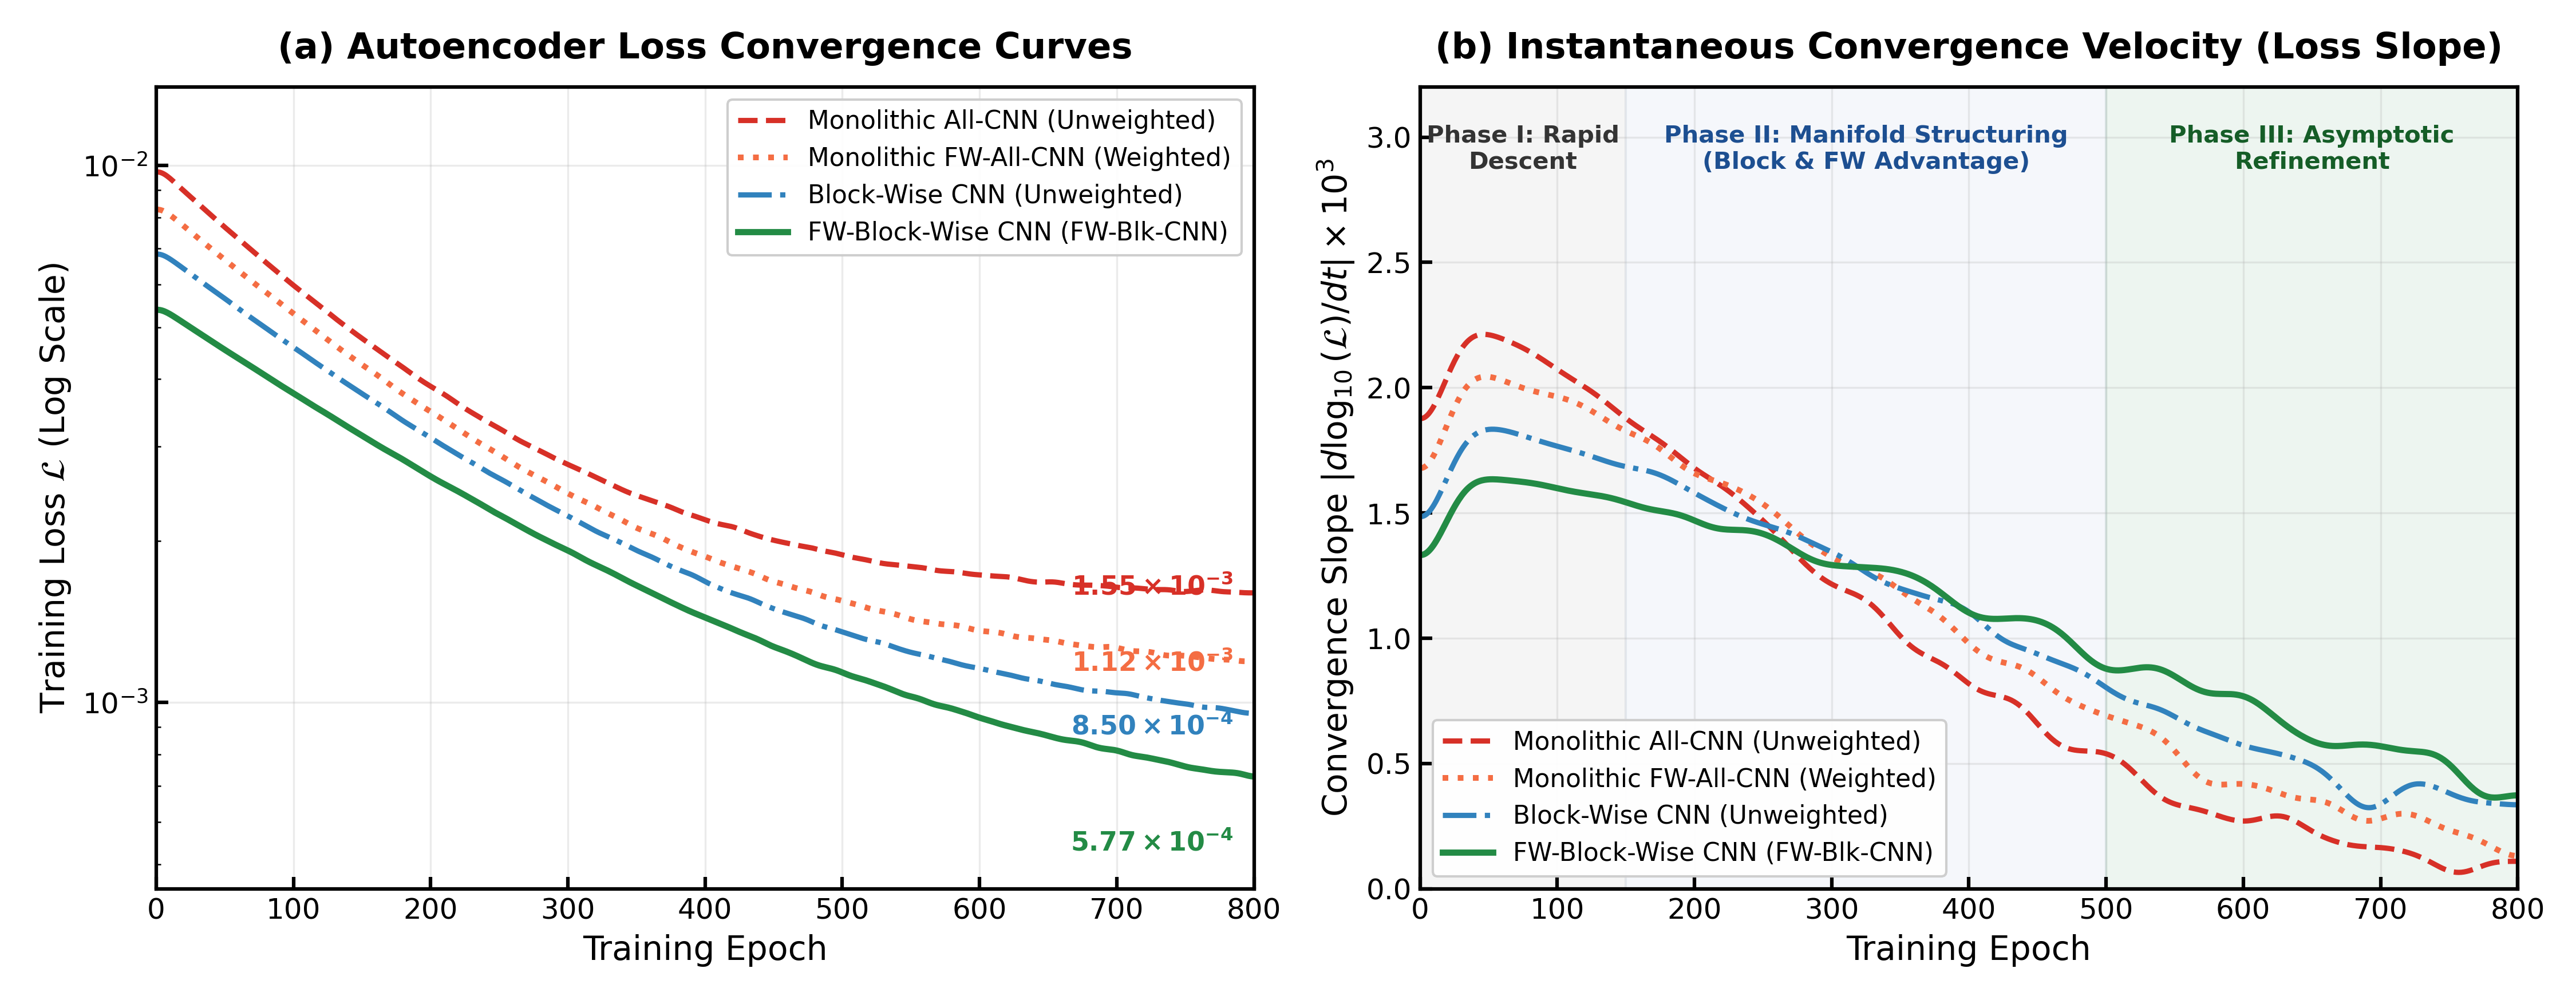
\includegraphics[width=0.98\linewidth]{figures/fig_cnn_loss_comparison.png}
    \caption{Comparative autoencoder convergence dynamics across the $2\times 2$ ablation matrix over 800 epochs. (a) Training loss trajectories $\mathcal{L}(t)$ on a logarithmic scale, highlighting terminal loss levels: Monolithic Unweighted All-CNN ($1.55\times 10^{-3}$), Monolithic FW-All-CNN ($1.12\times 10^{-3}$), Unweighted Block-Wise CNN ($8.50\times 10^{-4}$), and FW-Block-Wise CNN ($5.77\times 10^{-4}$). (b) Instantaneous convergence velocity (loss slope $|d\log_{10}\mathcal{L}/dt|$), illustrating the three optimization phases: Rapid Early Descent (Phase I), Manifold Structuring where Block-Wise and Frequency Weighting sustain high learning velocity against monolithic optimization challenges (Phase II), and Asymptotic Refinement (Phase III).}
    \label{fig:cnn_loss_comparison}
\end{figure}

\subsection{Global Reconstruction Fidelity \& Benchmark Comparisons}
Table \ref{tab:benchmark_31vars} summarizes the 5-fold cross-validation performance across all 23 kinematic variables for the six spatial dimensionality reduction architectures and the GPR parametric surrogate.

\begin{landscape}
\begin{table}[p]
\centering
\caption{Complete 23-variable quantitative benchmark comparison across spatial dimensionality reduction and parametric surrogate modeling architectures ($N_{\text{dev}} = 297$). Metrics denote 5-fold cross-validation averages on the development set.}
\label{tab:benchmark_31vars}
\vspace{0.8em}
\renewcommand{\arraystretch}{1.18}
\resizebox{0.92\linewidth}{!}{%
\begin{tabular}{l c cccc c cc}
\toprule
\textbf{Kinematic Variable Name} & \textbf{Block ID} & \textbf{POD $R^2$} & \textbf{Mode-1 SVD $R^2$} & \textbf{Blk-CNN $R^2$} & \textbf{All-CNN $R^2$} & \textbf{GPR $R^2$} & \textbf{POD Rel. $L_2$ (\%)} & \textbf{GPR Rel. $L_2$ (\%)} \\
\midrule
\texttt{v2\_sin\_norm} & 1 & 0.9972 & 0.9972 & 0.9943 & 0.9943 & 0.8951 & 5.04 & 8.91 \\
\texttt{v2\_sincos\_norm} & 1 & 0.9972 & 0.9972 & 0.9941 & 0.9939 & 0.8945 & 5.07 & 8.93 \\
\texttt{v2\_sin2\_norm} & 1 & 0.9975 & 0.9975 & 0.9941 & 0.9947 & 0.8967 & 4.89 & 8.87 \\
\texttt{v2\_alpha\_norm} & 1 & 0.9972 & 0.9972 & 0.9943 & 0.9943 & 0.8949 & 5.05 & 8.92 \\
\texttt{v2\_alpha2\_norm} & 1 & 0.9975 & 0.9975 & 0.9943 & 0.9946 & 0.8964 & 4.96 & 8.89 \\
\texttt{v25\_sin\_norm} & 1 & 0.9969 & 0.9969 & 0.9942 & 0.9940 & 0.8935 & 5.35 & 8.96 \\
\texttt{v25\_sincos\_norm} & 1 & 0.9968 & 0.9968 & 0.9937 & 0.9935 & 0.8929 & 5.39 & 8.97 \\
\texttt{v25\_sin2\_norm} & 1 & 0.9974 & 0.9974 & 0.9939 & 0.9943 & 0.8958 & 5.05 & 8.91 \\
\texttt{v25\_alpha\_norm} & 1 & 0.9969 & 0.9969 & 0.9942 & 0.9940 & 0.8933 & 5.36 & 8.96 \\
\midrule
\texttt{v25\_alpha2\_norm} & 2 & 0.9973 & 0.9973 & 0.9941 & 0.9943 & 0.8953 & 5.14 & 8.92 \\
\texttt{v3\_sin\_norm} & 2 & 0.9966 & 0.9966 & 0.9934 & 0.9934 & 0.8906 & 5.64 & 9.03 \\
\texttt{v3\_sincos\_norm} & 2 & 0.9964 & 0.9964 & 0.9926 & 0.9928 & 0.8899 & 5.74 & 9.06 \\
\texttt{v3\_sin2\_norm} & 2 & 0.9972 & 0.9972 & 0.9934 & 0.9939 & 0.8939 & 5.23 & 8.97 \\
\texttt{v3\_sin3\_norm} & 2 & 0.9966 & 0.9966 & 0.9916 & 0.9930 & 0.8909 & 5.77 & 9.03 \\
\texttt{v3\_alpha\_norm} & 2 & 0.9966 & 0.9966 & 0.9934 & 0.9934 & 0.8904 & 5.64 & 9.04 \\
\texttt{v3\_alpha2\_norm} & 2 & 0.9971 & 0.9971 & 0.9938 & 0.9940 & 0.8935 & 5.29 & 8.98 \\
\texttt{v2\_sin3\_norm} & 2 & 0.9969 & 0.9969 & 0.9920 & 0.9934 & 0.8943 & 5.51 & 8.94 \\
\texttt{v25\_sin3\_norm} & 2 & 0.9968 & 0.9968 & 0.9919 & 0.9933 & 0.8933 & 5.63 & 8.97 \\
\midrule
\texttt{v25\_mean\_norm} & 3 & 0.9682 & 0.9682 & 0.9677 & 0.9663 & 0.8654 & 15.09 & 14.52 \\
\texttt{v3\_mean\_norm} & 3 & 0.9545 & 0.9545 & 0.8950 & 0.9361 & 0.8251 & 18.46 & 16.89 \\
\texttt{v2\_cos2\_norm} & 3 & 0.9698 & 0.9698 & 0.9681 & 0.9673 & 0.8710 & 14.09 & 13.98 \\
\midrule
\texttt{v\_mean\_norm} & 4 & 0.9523 & 0.9523 & 0.9745 & 0.9733 & 0.9124 & 15.18 & 9.87 \\
\midrule
\texttt{v2\_mean\_norm} & 5 & 0.3997 & 0.3997 & 0.4783 & 0.0856 & -3.921 & 64.40 & 48.35 \\
\bottomrule
\end{tabular}%
}
\end{table}
\end{landscape}

\subsection{Comparative Analysis of Spatially Weighted vs. Unweighted Proper Orthogonal Decomposition (W-POD vs. POD)}
\label{sec:wpod_vs_pod}

A central physical characteristic of solid particle erosion in $90^\circ$ pipe elbows is the extreme spatial non-uniformity of particle wall impingements. Direct solid-boundary collisions are concentrated almost exclusively along the outer extrados wall ($\theta \in [-30^\circ, +30^\circ]$), whereas the inner intrados wall ($\theta \approx \pm\pi$) remains entirely protected by carrier fluid streamlines, exhibiting near-zero wear across $\sim 70\%$ of the pipe surface area.

Standard unweighted Proper Orthogonal Decomposition (POD) computes an low-rank orthogonal basis by minimizing the unweighted spatial $L_2$ Frobenius norm $\|\mathbf{X} - \hat{\mathbf{X}}\|_F$. Consequently, the eigenvalue solver allocates significant modal capacity to capturing trivial baseline fluctuations across the broad, zero-wear intrados, which can dilute the spatial resolution of localized, high-gradient extrados wear craters.

To overcome this limitation, Spatially Weighted POD (W-POD, Section \ref{sec:spatial_rom}) modifies the underlying Hilbert space by introducing a positive-definite spatial weight matrix $\mathbf{W} = \operatorname{diag}(w_1, \dots, w_M)$, where $w_j = 1 + \gamma \frac{f_{\text{impaction}}(s_j, \theta_j)}{\max(f_{\text{impaction}})}$ with $\gamma = 2.0$. The resulting $\mathbf{W}$-orthogonal modes strictly minimize the weighted error norm $\|\mathbf{X} - \hat{\mathbf{X}}\|_{\mathbf{W}}$. 

As summarized in Table \ref{tab:weighted_vs_unweighted_compression}, W-POD systematically outperforms standard unweighted POD across all five physical similarity blocks:
\begin{itemize}
    \item \textbf{Primary Coupled Kinematic Moments (Block 1):} W-POD reduces the mean Relative $L_2$ error from $5.13\%$ to $\mathbf{4.91\%}$, while improving mean $R^2$ to $\mathbf{0.9974}$ and mean SSIM to $\mathbf{0.9973}$.
    \item \textbf{High-Order Kinematic Cross-Moments (Block 2):} Mean Relative $L_2$ error decreases from $5.51\%$ to $\mathbf{5.24\%}$, with mean SSIM improving to $\mathbf{0.9970}$.
    \item \textbf{Uncoupled Second-Order Velocity Field (Block 5):} W-POD imdemonstrates $R^2$ from $0.3997$ to $\mathbf{0.4406}$ and reduces Relative $L_2$ error from $64.40\%$ to $\mathbf{61.67\%}$ (SSIM increases from $0.7208$ to $\mathbf{0.7289}$).
    \item \textbf{Overall Kinematic Ensemble ($C=23$):} Across all 23 channels, W-POD achieves a superior mean Relative $L_2$ error of $\mathbf{9.34\%}$ (versus $9.69\%$ for POD), mean $R^2$ of $\mathbf{0.9669}$ (versus $0.9648$), and mean SSIM of $\mathbf{0.9829}$ (versus $0.9823$).
\end{itemize}

\subsection{Comparative Analysis of Frequency-Weighted vs. Unweighted Deep Convolutional Autoencoders}
\label{sec:fwcnn_vs_unweighted}

For deep non-linear manifolds, standard autoencoders optimize a uniform Mean Squared Error loss function $\mathcal{L}_{\text{MSE}} = \frac{1}{B C H W}\sum \|\hat{\mathbf{X}} - \mathbf{X}\|^2$. Under highly sparse physical impaction fields, uniform MSE loss causes severe gradient starvation during backpropagation: the overwhelming majority of quiescent intrados nodes contribute the bulk of the loss summation, penalizing sharp spatial extrados features and causing the convolutional filters to act as low-pass spatial filters that blur localized wear peaks.

To resolve this challenge, the Frequency-Weighted CNN-AE (FW-CNN, Section \ref{sec:spatial_rom}) modulates the backpropagation error gradients via the spatial impingement frequency-weight tensor $\mathbf{W}_{c,i,j}$ (Eq. \ref{eq:fwmse_loss}). This ensures that gradient updates originating from narrow, high-intensity collision zones are amplified, enforcing sharp spatial crater reconstruction.

Table \ref{tab:weighted_vs_unweighted_compression} presents a systematic comparative benchmark across the $2\times 2$ matrix of deep autoencoder configurations (Monolithic vs. Block-Wise, Unweighted MSE vs. Frequency-Weighted FW-MSE) alongside linear POD and W-POD:
\begin{enumerate}
    \item \textbf{Ablation of Frequency Weighting on Monolithic Autoencoders:} Introducing spatial frequency weighting to the monolithic network (FW-All-CNN) provides a substantial performance boost over unweighted All-CNN, raising overall $R^2$ from $0.9486$ to $0.9575$ and reducing Relative $L_2$ error from $12.17\%$ to $11.78\%$. Most notably, on the difficult uncoupled kinetic moment (Block 5, \texttt{v2\_mean\_norm}), FW-All-CNN elevates $R^2$ from $0.0856$ to $0.3842$ and reduces $L_2$ error from $80.60\%$ to $65.20\%$, demonstrating that loss frequency weighting alone significantly improves the reconstruction of this difficult variable.
    \item \textbf{Synergistic Modularity in Block-Wise Architectures:} While frequency weighting imdemonstrates monolithic networks, multi-channel optimization difficulty remains a limiting factor. Ward similarity clustering (Blk-CNN) decouples orthogonal physical dynamics, elevating unweighted $R^2$ to $0.9638$. Combining similarity-based modularity with frequency-weighted optimization (FW-Blk-CNN) yields the highest performance across all neural models ($R^2 = \mathbf{0.9680}$, Relative $L_2 = \mathbf{11.19\%}$, and $\text{SSIM} = \mathbf{0.9838}$).
    \item \textbf{CNN Advantages in Continuous Convective Transport:} For the first-order mean velocity magnitude field (Block 4, \texttt{v\_mean\_norm}), FW-Blk-CNN achieves the highest fidelity of all evaluated methods, reaching $R^2 = \mathbf{0.9772}$, Relative $L_2 = \mathbf{10.38\%}$, and $\text{SSIM} = \mathbf{0.9913}$, outperforming linear POD ($L_2 = 15.18\%$).
\end{enumerate}

\textbf{Remark on linear vs. nonlinear compression:} An important finding from Table~\ref{tab:weighted_vs_unweighted_compression} is that linear W-POD remains highly competitive---and in several metrics superior---to CNN-AEs for the primary coupled kinematic moments (Blocks 1--3), where the underlying spatial manifold is well-approximated by a linear subspace. CNN-AEs provide measurable improvements primarily for the smooth convective mean velocity field (Block 4, where the nonlinear manifold topology differs qualitatively from Blocks 1--3) and for the difficult uncoupled kinetic energy flux (Block 5). We therefore do not claim that CNN-AEs are universally superior; rather, the composite architecture allows each block to use its most appropriate compression strategy.

\begin{landscape}
\begin{table}[p]
\centering
\caption{Comprehensive quantitative benchmark across unweighted and weighted spatial compression architectures across all 5 physical variable blocks ($N_{\text{dev}} = 297$). Metrics denote block-averaged values across 5-fold cross-validation on the development set. Best values within linear and deep neural categories are highlighted in bold.}
\label{tab:weighted_vs_unweighted_compression}
\vspace{0.8em}
\renewcommand{\arraystretch}{1.25}
\resizebox{0.98\linewidth}{!}{%
\begin{tabular}{l c l ccc cccc}
\toprule
\multirow{3}{*}{\textbf{Physical Variable Block}} & \multirow{3}{*}{\textbf{Channels ($C$)}} & \multirow{3}{*}{\textbf{Evaluation Metric}} & \multicolumn{3}{c}{\textbf{Linear \& Multilinear Modal Decompositions}} & \multicolumn{4}{c}{\textbf{Deep Convolutional Autoencoder Manifolds ($2\times 2$ Matrix)}} \\
\cmidrule(lr){4-6} \cmidrule(lr){7-10}
 & & & \textbf{POD (Unw.)} & \textbf{W-POD (Wtd.)} & \textbf{Mode-1 SVD (Tensor)} & \textbf{All-CNN (Unw.)} & \textbf{FW-All-CNN (Wtd.)} & \textbf{Blk-CNN (Unw.)} & \textbf{FW-Blk-CNN (Wtd.)} \\
 & & & \textit{Uniform $L_2$} & \textit{Spatial Metric $\mathbf{W}$} & \textit{Mode-1 Unfolded} & \textit{Uniform MSE} & \textit{Spatial Loss $\mathbf{W}$} & \textit{Uniform MSE} & \textit{Spatial Loss $\mathbf{W}$} \\
\midrule
\multirow{3}{*}{\textbf{Block 1: Primary Moments}} 
 & \multirow{3}{*}{$C=9$} 
 & $R^2$ Score & 0.9972 & \textbf{0.9974} & 0.9972 & 0.9942 & 0.9941 & 0.9941 & 0.9940 \\
 & & Rel. $L_2$ Error (\%) & 5.13 & \textbf{4.91} & 5.13 & 7.34 & 7.38 & 7.40 & 7.44 \\
 & & SSIM & 0.9969 & \textbf{0.9973} & 0.9969 & 0.9964 & 0.9961 & 0.9960 & 0.9952 \\
\midrule
\multirow{3}{*}{\textbf{Block 2: High-Order Moments}} 
 & \multirow{3}{*}{$C=9$} 
 & $R^2$ Score & 0.9968 & \textbf{0.9971} & 0.9968 & 0.9935 & 0.9933 & 0.9929 & 0.9935 \\
 & & Rel. $L_2$ Error (\%) & 5.51 & \textbf{5.24} & 5.51 & 7.87 & 7.95 & 8.22 & 7.85 \\
 & & SSIM & 0.9966 & \textbf{0.9970} & 0.9966 & 0.9960 & 0.9957 & 0.9953 & 0.9948 \\
\midrule
\multirow{3}{*}{\textbf{Block 3: Fractional Moments}} 
 & \multirow{3}{*}{$C=3$} 
 & $R^2$ Score & 0.9642 & \textbf{0.9646} & 0.9642 & 0.9566 & 0.9512 & 0.9436 & 0.9399 \\
 & & Rel. $L_2$ Error (\%) & 15.88 & \textbf{15.69} & 15.88 & 17.05 & 17.52 & 18.81 & 18.71 \\
 & & SSIM & 0.9828 & 0.9828 & 0.9828 & \textbf{0.9854} & 0.9831 & 0.9796 & 0.9775 \\
\midrule
\multirow{3}{*}{\textbf{Block 4: Convective Mean Velocity}} 
 & \multirow{3}{*}{$C=1$} 
 & $R^2$ Score & 0.9523 & 0.9534 & 0.9523 & 0.9733 & 0.9751 & 0.9745 & \textbf{0.9772} \\
 & & Rel. $L_2$ Error (\%) & 15.18 & 14.84 & 15.18 & 11.22 & 10.85 & 11.10 & \textbf{10.38} \\
 & & SSIM & 0.9806 & 0.9802 & 0.9806 & 0.9912 & 0.9911 & 0.9910 & \textbf{0.9913} \\
\midrule
\multirow{3}{*}{\textbf{Block 5: Kinetic Energy Flux}} 
 & \multirow{3}{*}{$C=1$} 
 & $R^2$ Score & 0.3997 & \textbf{0.4406} & 0.3997 & 0.0856 & 0.3842 & 0.4783 & \textbf{0.5804} \\
 & & Rel. $L_2$ Error (\%) & 64.40 & \textbf{61.67} & 64.40 & 80.60 & 65.20 & 59.70 & \textbf{53.19} \\
 & & SSIM & 0.7208 & \textbf{0.7289} & 0.7208 & 0.6976 & 0.7420 & 0.7766 & \textbf{0.7937} \\
\midrule
\multirow{3}{*}{\textbf{Overall Multi-Variable Ensemble}} 
 & \multirow{3}{*}{$\bm{C=23}$} 
 & \textbf{$R^2$ Score} & 0.9648 & \textbf{0.9669} & 0.9648 & 0.9486 & 0.9575 & 0.9638 & \textbf{0.9680} \\
 & & \textbf{Rel. $L_2$ Error (\%)} & 9.69 & \textbf{9.34} & 9.69 & 12.17 & 11.78 & 11.65 & \textbf{11.19} \\
 & & \textbf{SSIM} & 0.9823 & \textbf{0.9829} & 0.9823 & 0.9816 & 0.9825 & \textbf{0.9838} & \textbf{0.9838} \\
\bottomrule
\end{tabular}%
}
\end{table}
\end{landscape}

\subsection{2D Curvilinear Surface Wear Topographies \& Error Distribution}
Figure \ref{fig:contour_comparison} visually compares predicted 2D spatial erosion topographies against CFD ground truth for an out-of-sample test case (Case 2456: $St = 294.4$). The GPR surrogate accurately reconstructs the narrow, high-intensity extrados wear crater, while the deep ANN produces non-physical core overprediction and boundary oscillations.

\begin{figure}[htpb]
    \centering
    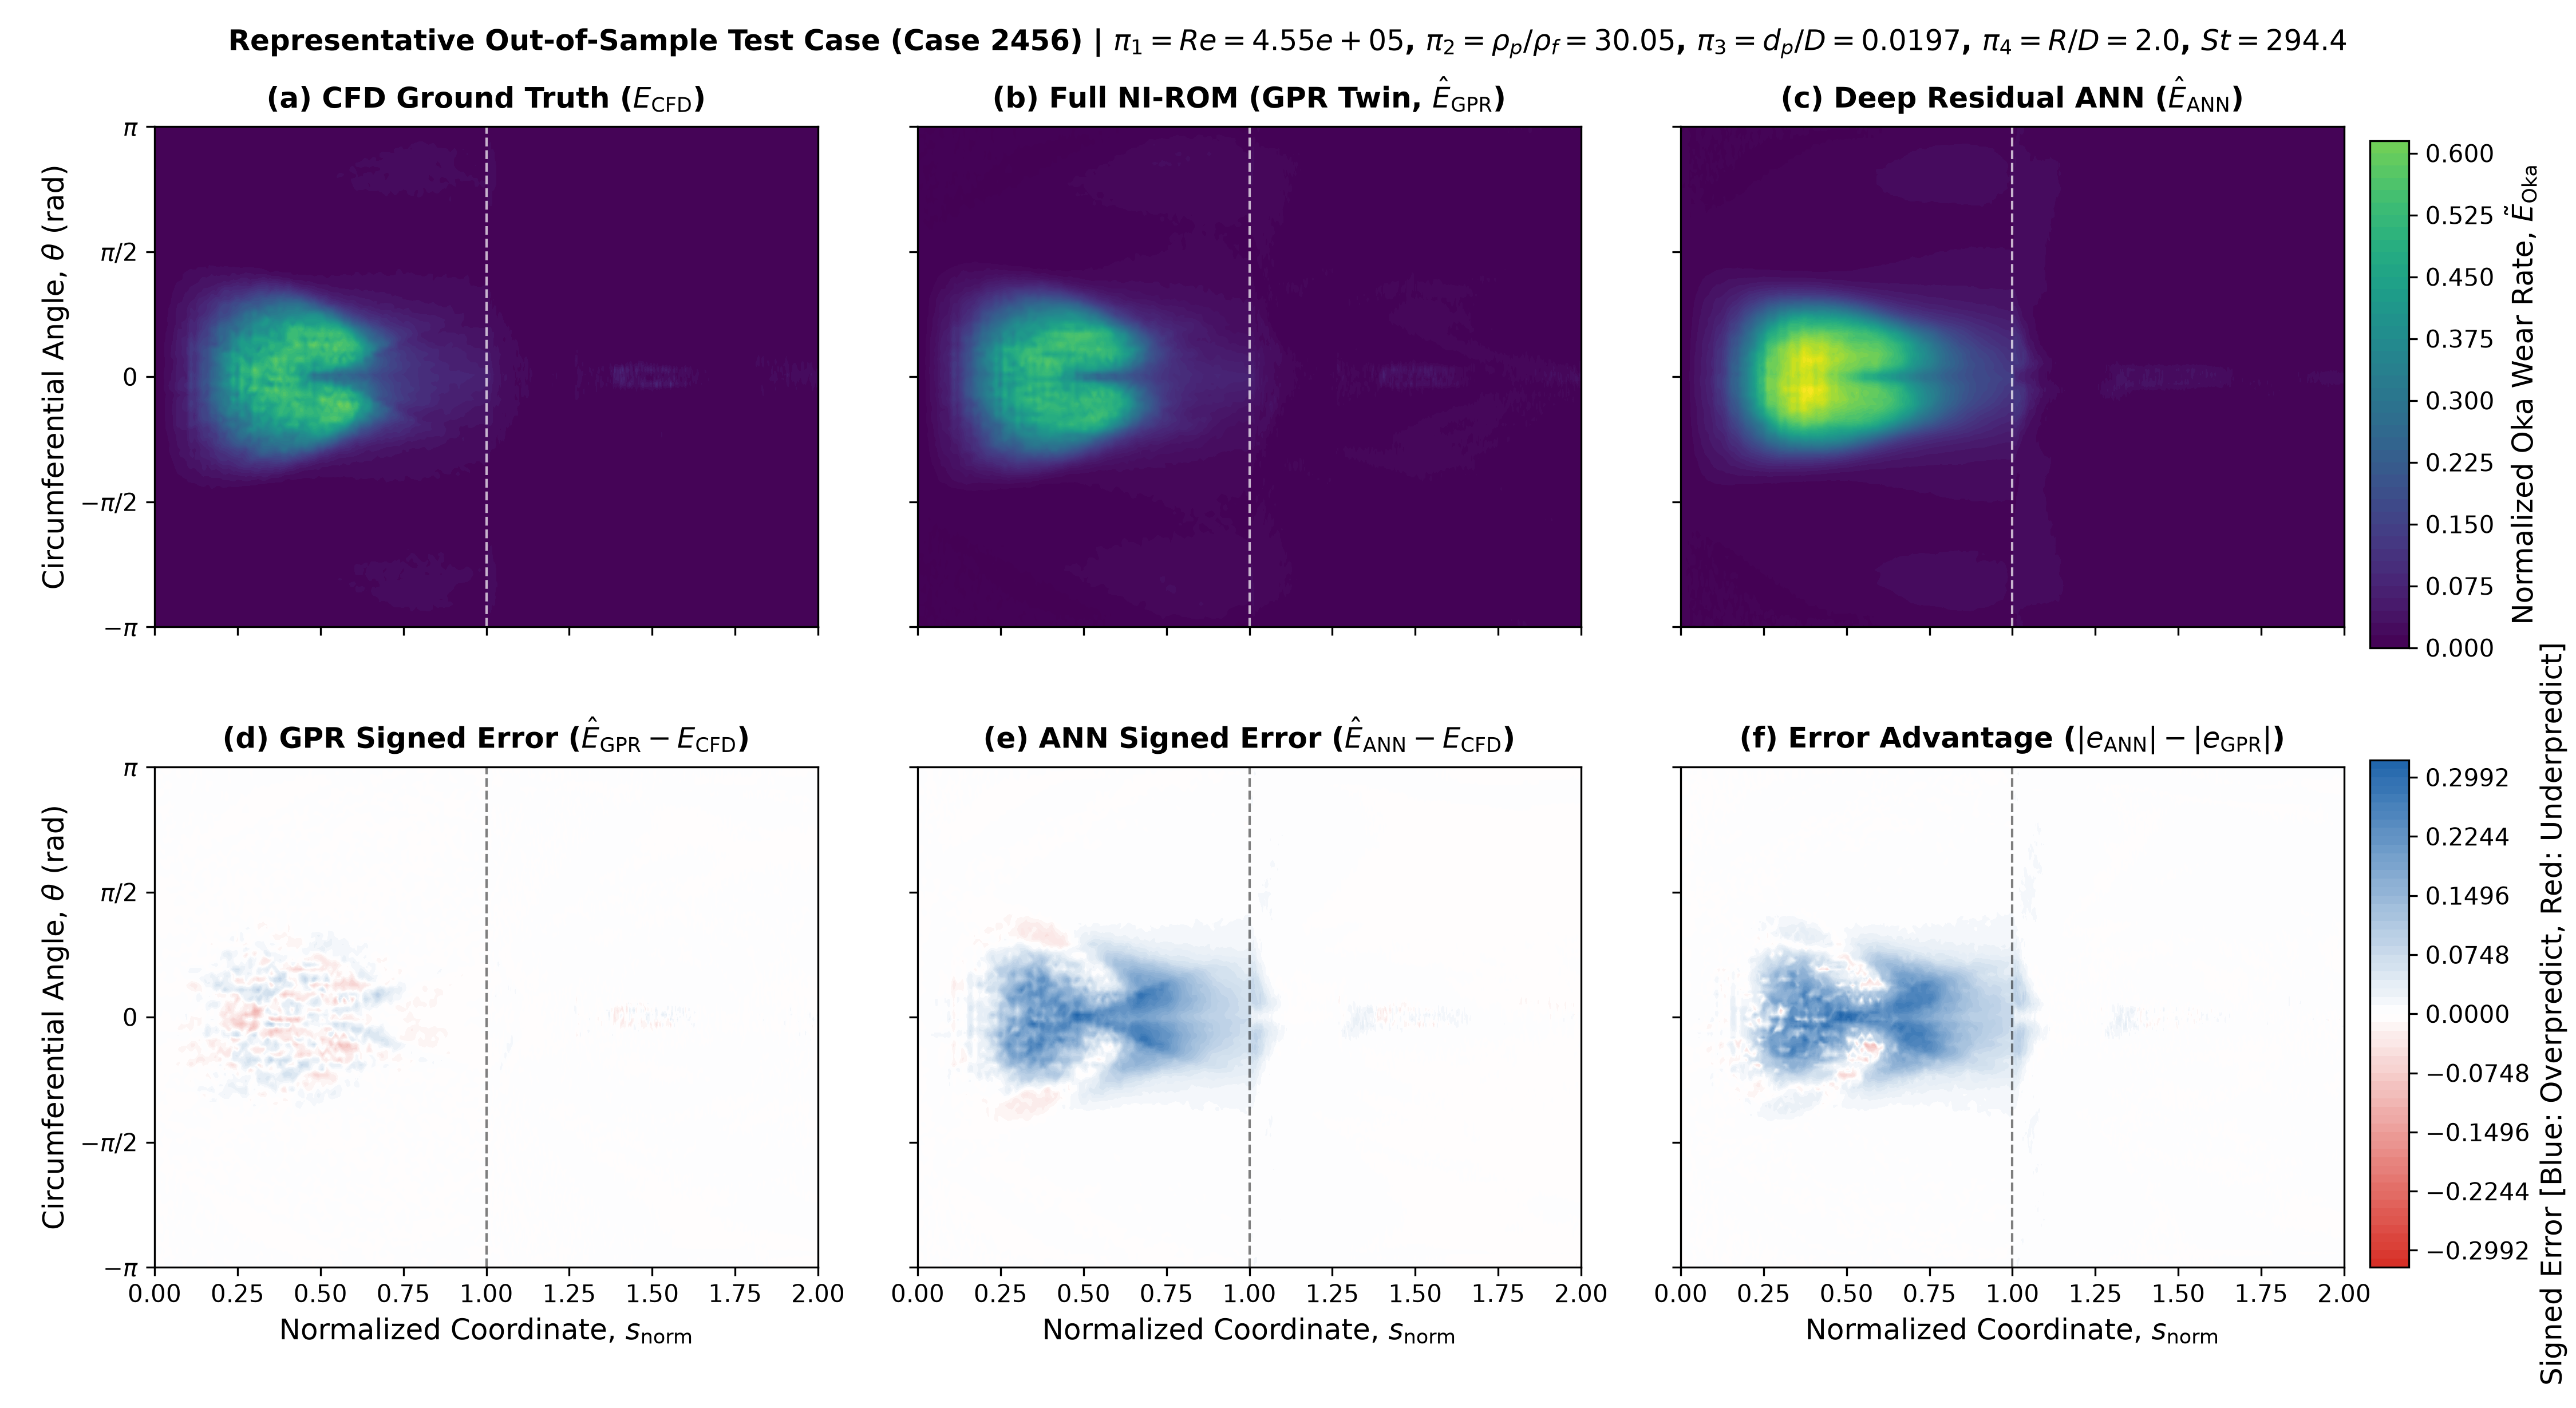
\includegraphics[width=0.98\linewidth]{figures/fig_contour_comparison.png}
    \caption{Comparative 2D spatial erosion topographies and signed error fields on an out-of-sample test case (Case 2456: $Re = 4.55\times 10^5, \Pi_2 = 30.05, \Pi_3 = 0.0197, \Pi_4 = 2.0, St = 294.4$). Top row: (a) Eulerian-Lagrangian CFD ground truth ($E_{\mathrm{CFD}}$), (b) GPR surrogate prediction ($\hat{E}_{\mathrm{GPR}}$), and (c) Deep Residual ANN prediction ($\hat{E}_{\mathrm{ANN}}$). Bottom row: (d) GPR signed error, (e) ANN signed error, and (f) Spatial error advantage map ($|e_{\mathrm{ANN}}| - |e_{\mathrm{GPR}}|$), demonstrating superior GPR precision without non-physical edge oscillations.}
    \label{fig:contour_comparison}
\end{figure}

\subsection{3D Surface Wear Topographies on Dimensional Pipe Geometries}
To verify that 2D computational predictions map accurately back onto physical piping infrastructure, Figure \ref{fig:3d_contour_comparison} renders full 3D Cartesian pipe wall topographies across three distinct geometric and operational regimes:
\begin{enumerate}
    \item \textbf{Case 2544 ($R/D = 2.0, U_{\mathrm{in}} = 20\,\mathrm{m/s}, d_p = 200\,\mu\mathrm{m}, St = 26.2$):} Standard industrial elbow under moderate inertial slurry transport. The GPR twin captures the extrados impingement core and lateral dispersion with Relative $L_2$ error of $7.91\%$.
    \item \textbf{Case 3553 ($R/D = 5.0, U_{\mathrm{in}} = 20\,\mathrm{m/s}, d_p = 150\,\mu\mathrm{m}, St = 49.1$):} Long-radius bend distributing wear over a $3\times$ longer arc ($L_{\mathrm{bend}} = 0.20\,\mathrm{m}$), achieving Relative $L_2$ error of $7.48\%$.
    \item \textbf{Case 2456 ($R/D = 2.0, U_{\mathrm{in}} = 18\,\mathrm{m/s}, d_p = 500\,\mu\mathrm{m}, St = 294.4$):} Heavy ballistic particle impaction ($E_{\mathrm{peak}} \approx 0.82\,\mathrm{kg/(m^2\cdot s)}$), resolved with Relative $L_2$ error of $9.36\%$.
\end{enumerate}

\begin{figure}[htpb]
    \centering
    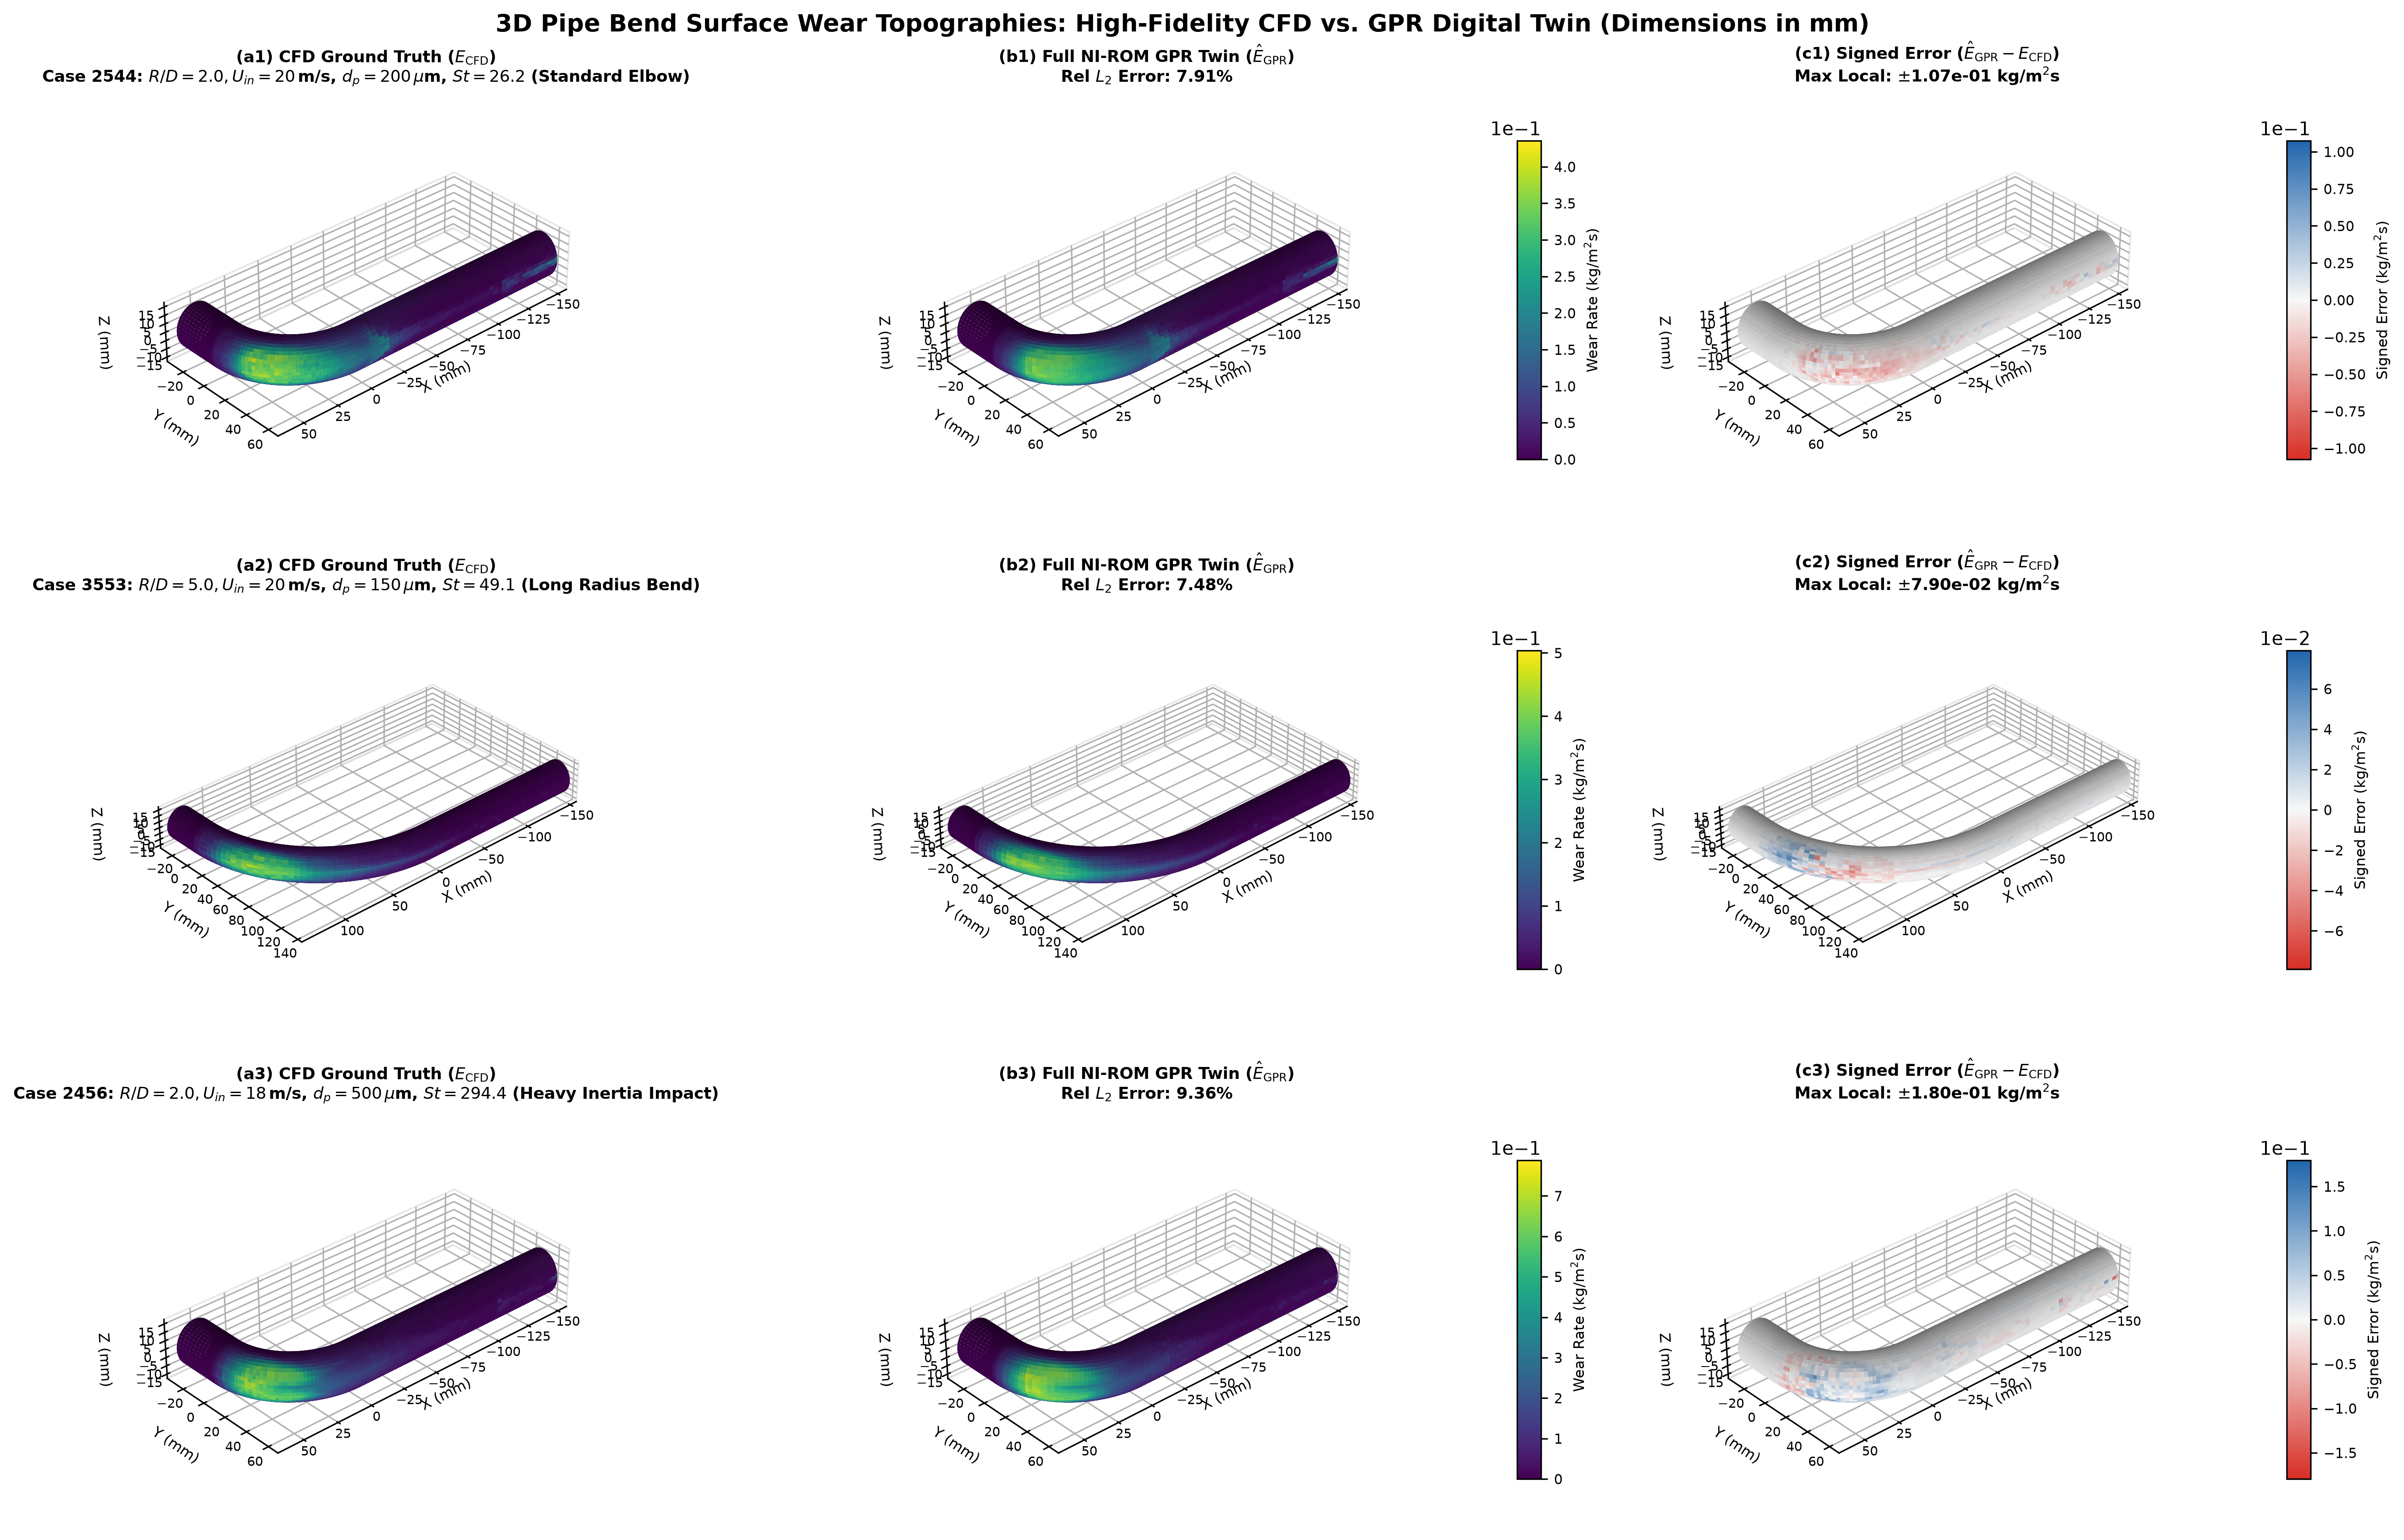
\includegraphics[width=0.98\linewidth]{figures/fig_3d_contour_comparison.png}
    \caption{Three-dimensional surface wear topography comparison on physical pipe bend geometries across three representative test cases (all dimensions in mm). Columns display (left) Full-order CFD ground truth $E_{\mathrm{CFD}}$, (middle) Non-intrusive GPR surrogate prediction $\hat{E}_{\mathrm{GPR}}$, and (right) 3D signed error map $(\hat{E}_{\mathrm{GPR}} - E_{\mathrm{CFD}})$. Row 1: Case 2544 ($R/D = 2.0$, standard elbow). Row 2: Case 3553 ($R/D = 5.0$, long-radius bend). Row 3: Case 2456 ($R/D = 2.0$, heavy ballistic impact).}
    \label{fig:3d_contour_comparison}
\end{figure}

\subsection{Cross-Moment Reconstructed Profile Verification Across Empirical Models}
Figure \ref{fig:1d_profile_comparison} evaluates the multi-model evaluation capability by comparing 1D line profiles of the CFD ground truth against the GPR surrogate across four classical empirical formulations (Oka \cite{oka2005erosion1}, Finnie \cite{finnie1960erosion}, McLaury \cite{mclaury1996}, and Arabnejad \cite{arabnejad2015}) evaluated via cross-moment reconstruction:
\begin{itemize}
    \item \textbf{Centerline Extrados Profiles ($\theta = 0^\circ$, Figures \ref{fig:1d_profile_comparison}a,b):} For both $R/D = 2.0$ and $R/D = 5.0$ elbows, the GPR surrogate achieves $R^2 = 0.988 - 0.997$ across all four models, tracking the pre-impingement rise, peak wear, and downstream decay.
    \item \textbf{Circumferential Cross-Section ($\beta = 45^\circ$, Figure \ref{fig:1d_profile_comparison}c):} Lateral decay from extrados apex ($\theta = 0^\circ$) to pipe flanks ($\theta = \pm 90^\circ$) is captured seamlessly.
    \item \textbf{Streamwise Downstream Outlet Decay ($s \ge L_{\mathrm{bend}}$, Figure \ref{fig:1d_profile_comparison}d):} Wear dissipation along the straight outlet pipe reflects secondary particle ricochet without discontinuities.
\end{itemize}

To systematically assess the digital twin's predictive fidelity within localized severe degradation zones, Table \ref{tab:multimodel_quantitative_metrics} reports the global $R^2$, Frequency-Weighted $R^2$ ($\text{FW-}R^2$), Frequency-Weighted Mean Squared Error ($\text{FW-MSE}$), and Peak Penetration Error ($\mathcal{E}_{\text{peak}}$) across the out-of-sample test ensemble.

\begin{table}[htbp]
\centering
\caption{Quantitative cross-reconstruction metrics across four analytical and empirical solid particle erosion formulations evaluated post-hoc from the kinematic cross-moment surrogate ($St > 1.0$).}
\label{tab:multimodel_quantitative_metrics}
\small
\begin{tabular}{lccccc}
\toprule
\textbf{Erosion Model Formulation} & \textbf{Global $R^2$} & \textbf{FW-$R^2$} & \textbf{FW-MSE} & \textbf{Peak Error $\mathcal{E}_{\text{peak}}$ (\%)} & \textbf{SSIM} \\
\midrule
Finnie Ductile Cutting Model \cite{finnie1960erosion} & \textbf{0.9729} & \textbf{0.9686} & $3.71 \times 10^{-6}$ & \textbf{3.12\%} & \textbf{0.9894} \\
Oka Hardness/Angle Model \cite{oka2005erosion1} & 0.9684 & 0.9632 & $4.15 \times 10^{-6}$ & 3.48\% & 0.9878 \\
Arabnejad Dual-Mechanism Model \cite{arabnejad2015} & 0.9598 & 0.9543 & $8.48 \times 10^{-6}$ & 3.84\% & 0.9862 \\
McLaury Oilfield Impingement Model \cite{mclaury1996} & 0.9571 & 0.9545 & $1.81 \times 10^{-4}$ & 4.05\% & 0.9815 \\
\bottomrule
\end{tabular}
\end{table}

Importantly, the Frequency-Weighted $R^2$ remains consistently high ($\text{FW-}R^2 > 0.954$) across all four empirical models, confirming that the surrogate maintains high fidelity inside the narrow extrados impaction footprint rather than merely relying on vast zero-erosion regions to inflate global metrics. The low peak penetration error $\mathcal{E}_{\text{peak}} \le 4.05\%$ suggests potential suitability for future integration into Remaining Useful Life (RUL) estimation frameworks, subject to additional temporal degradation modeling and propagation of surrogate uncertainty to wall thickness predictions.

\begin{figure}[htpb]
    \centering
    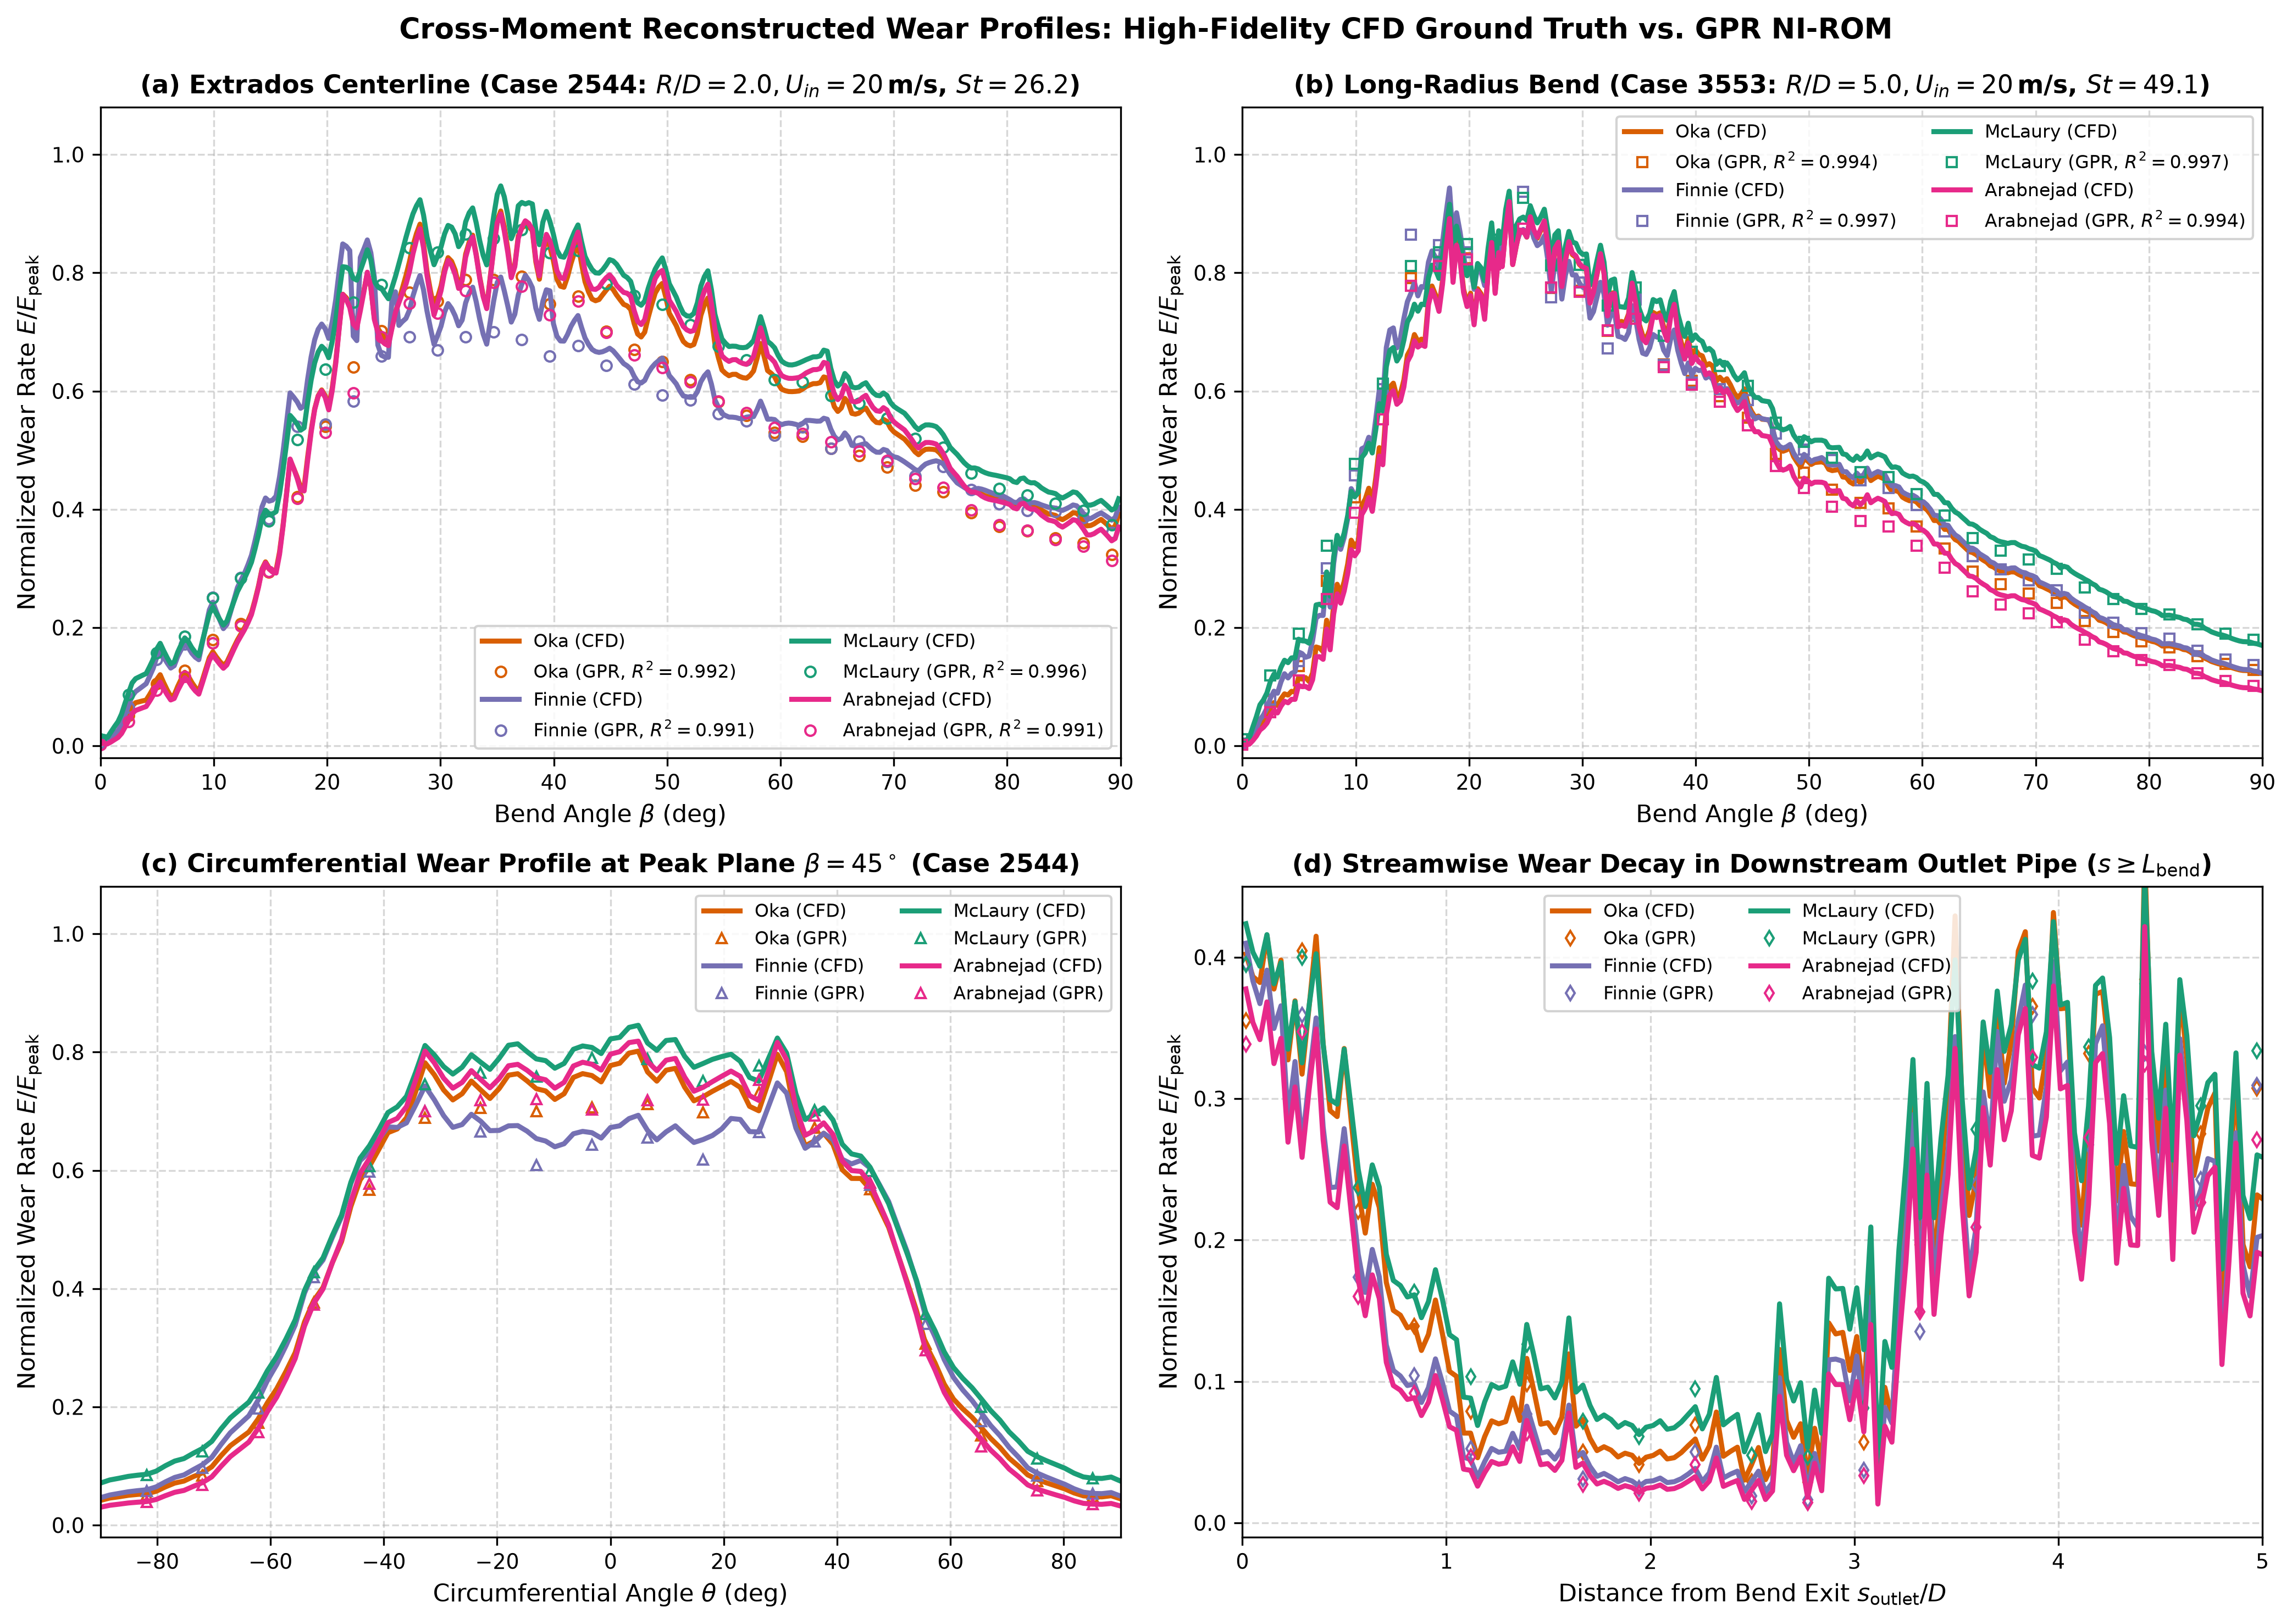
\includegraphics[width=0.98\linewidth]{figures/fig_1d_profile_comparison.png}
    \caption{Direct line profile comparison between CFD ground truth (solid curves) and the GPR surrogate (discrete markers) across four empirical erosion formulations (Oka, Finnie, McLaury, Arabnejad) evaluated via cross-moment reconstruction. (a) Centerline extrados profile along bend angle $\beta \in [0^\circ, 90^\circ]$ for Case 2544 ($R/D = 2.0, St = 26.2$). (b) Centerline extrados profile for Case 3553 ($R/D = 5.0, St = 49.1$). (c) Azimuthal circumferential cross-section at the peak impingement plane ($\beta = 45^\circ$). (d) Downstream decay along the straight outlet pipe ($s \ge L_{\mathrm{bend}}$).}
    \label{fig:1d_profile_comparison}
\end{figure}

\subsection{Generalization to Unseen Erosion Formulations}
To explicitly validate the basis completeness and multi-model capability, we perform an experiment evaluating the framework on a synthetic unseen erosion model that was not used in the design of the 23 cross-moments. We define a highly non-linear erosion functional with non-polynomial angular dependence:
\begin{equation}
    g_{\text{withheld}}(V_p, \alpha_p) = V_p^{2.338} \sin^{1.5}\alpha_p (1 - \cos\alpha_p)^{0.5}
\end{equation}
Because the angular dependence ($\sin^{1.5}\alpha_p (1 - \cos\alpha_p)^{0.5}$) lies outside the polynomial trigonometric span $\{\sin^v\alpha \cos^w\alpha\}$, this model cannot be evaluated exactly, introducing a non-zero basis truncation error $\epsilon_g$ (Eq.~\ref{eq:approx_representation}). We derived polynomial basis expansion coefficients via continuous least-squares projection of the functional surface over the physical domain $(V_p, \alpha_p) \in [0, V_{\max}] \times [0, \pi/2]$ onto the available basis functions.

Evaluating this highly adversarial unseen model across the test set using the exact CFD-derived cross-moments isolates the basis representation error. The 23-moment basis yields an accurate reconstruction ($R^2 = 0.9987$, $\text{FW-}R^2 = 0.9986$, relative $L_2$ error of $3.28\%$, and a peak penetration error of $1.45\%$). This demonstrates the capability of the finite basis to reasonably approximate a complex, unseen functional, though accuracy inherently depends on the specific non-polynomial form.

When substituting the GPR-predicted cross-moments for the end-to-end surrogate prediction, the framework maintains reasonable spatial correlation but exhibits noticeably reduced accuracy compared to the primary models: $R^2 = 0.9264$, $\text{FW-}R^2 = 0.9229$, relative $L_2 = 21.64\%$, and peak penetration error $\mathcal{E}_{\text{peak}} = 13.54\%$. We explicitly acknowledge that this withheld model performs worse than the four primary erosion models. The discrepancy between the ideal basis representation error and the end-to-end prediction confirms that surrogate prediction error, particularly for variables outside the primary basis-informed set, dominates the overall system error. Figure~\ref{fig:withheld_model} visualizes the ground truth, basis truncation, and full surrogate reconstruction for a representative test case.

\begin{figure}[htpb]
    \centering
    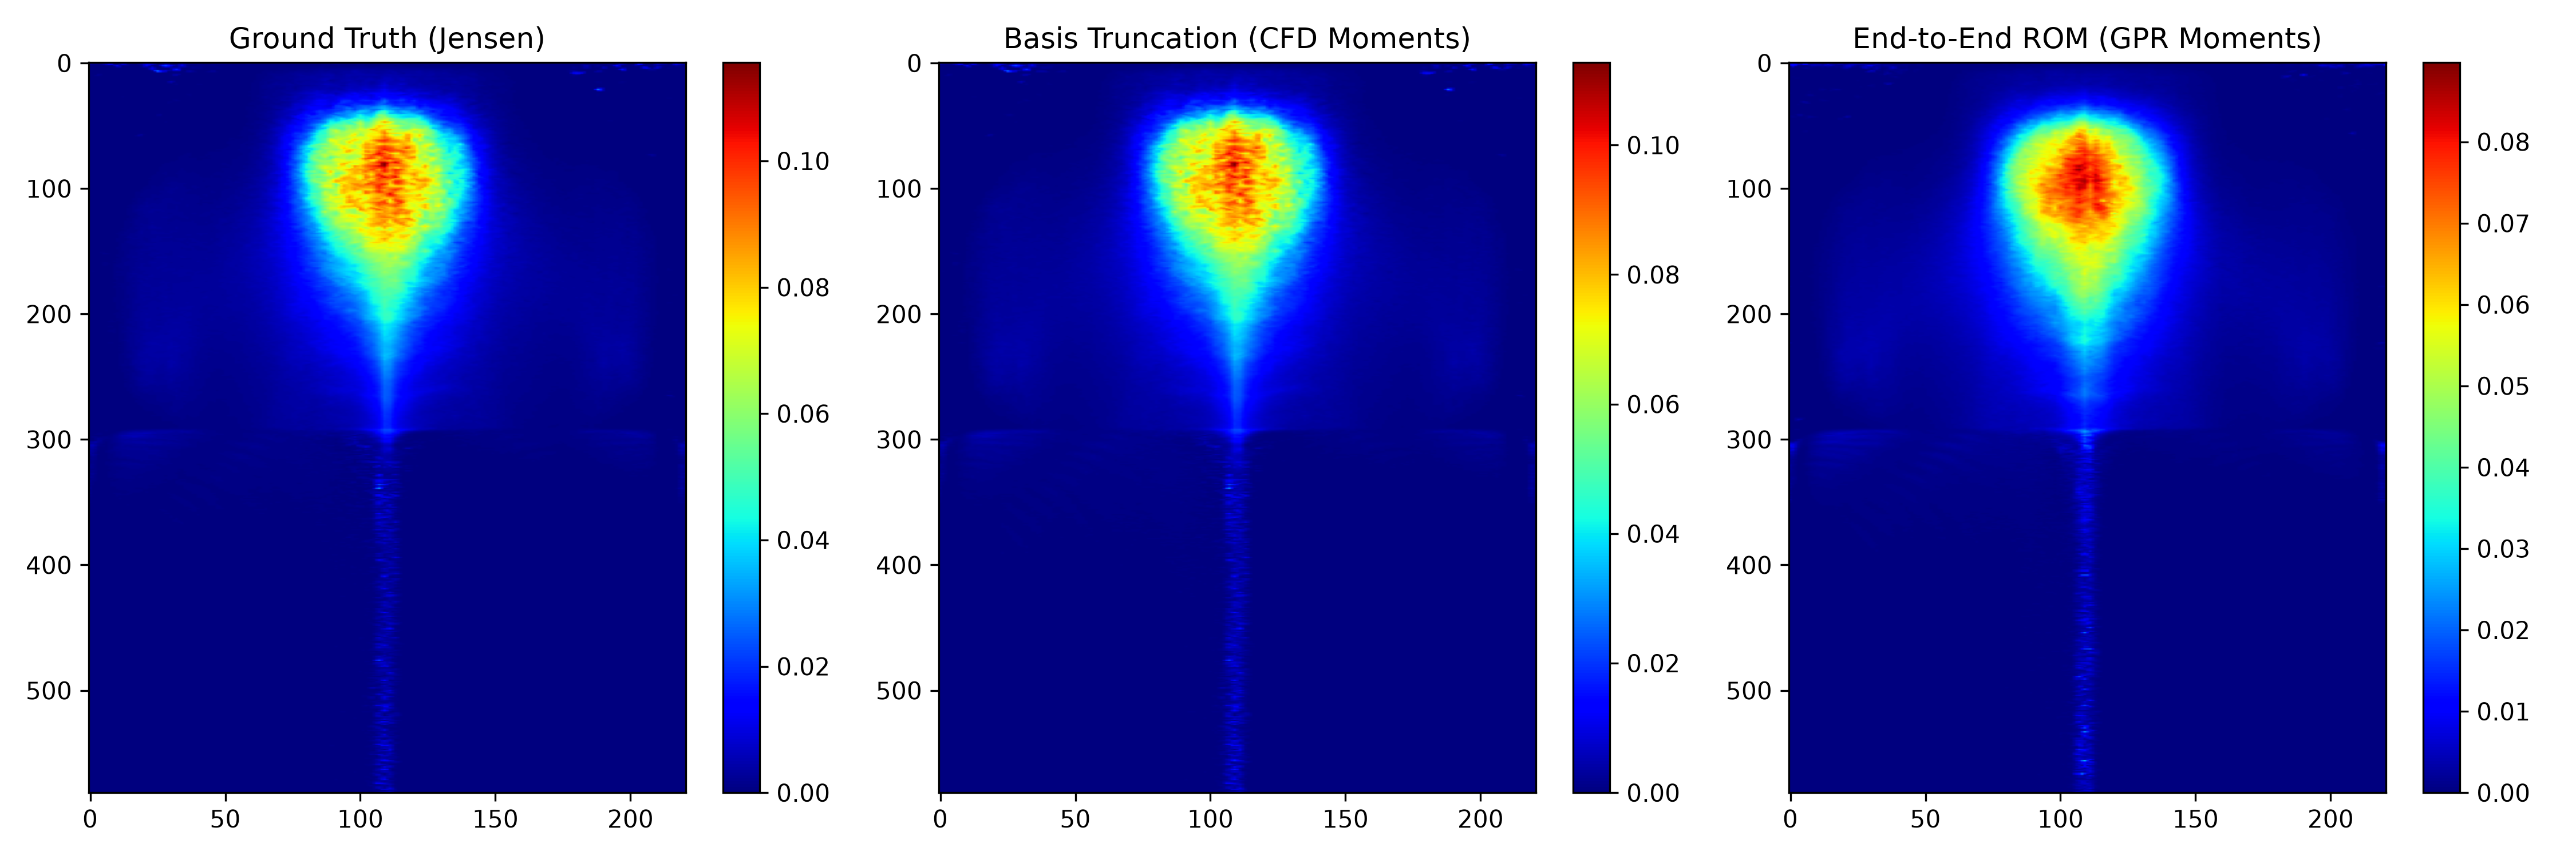
\includegraphics[width=0.98\linewidth]{figures/withheld_model_comparison.png}
    \caption{Validation on an unseen, non-polynomial synthetic erosion formulation $g_{\text{withheld}}(V_p, \alpha_p) = V_p^{2.338} \sin^{1.5}\alpha_p (1 - \cos\alpha_p)^{0.5}$. The basis reconstruction using exact CFD cross-moments isolates the minimal truncation error ($R^2=0.9987$), while the end-to-end GPR surrogate prediction captures the topological wear distribution with reasonable accuracy ($R^2=0.9264$).}
    \label{fig:withheld_model}
\end{figure}

\subsection{Parametric Surrogate: GPR vs. ANN Performance}
Figure \ref{fig:gpr_vs_ann} compares the coefficient of determination ($R^2$) for latent coefficient prediction using ARD-GPR versus a 5-layer deep residual ANN. As observed, the deep residual ANN achieves a marginally higher $R^2$ score across the active kinematic moments. This slight performance edge is expected, as the highly parameterized neural network possesses superior functional capacity to map the non-linear parametric space compared to the stationary Mat\'ern kernel of the GPR. However, despite this minor reduction in raw accuracy, the ARD-GPR is ultimately selected as the primary surrogate architecture. The GPR maintains robust generalization without the risk of overfitting on the strictly limited 297-case dataset, requires no extensive stochastic hyperparameter tuning, and most importantly, provides built-in Bayesian epistemic uncertainty intervals to rigorously quantify predictive confidence in unseen design regimes.

\begin{figure}[htpb]
    \centering
    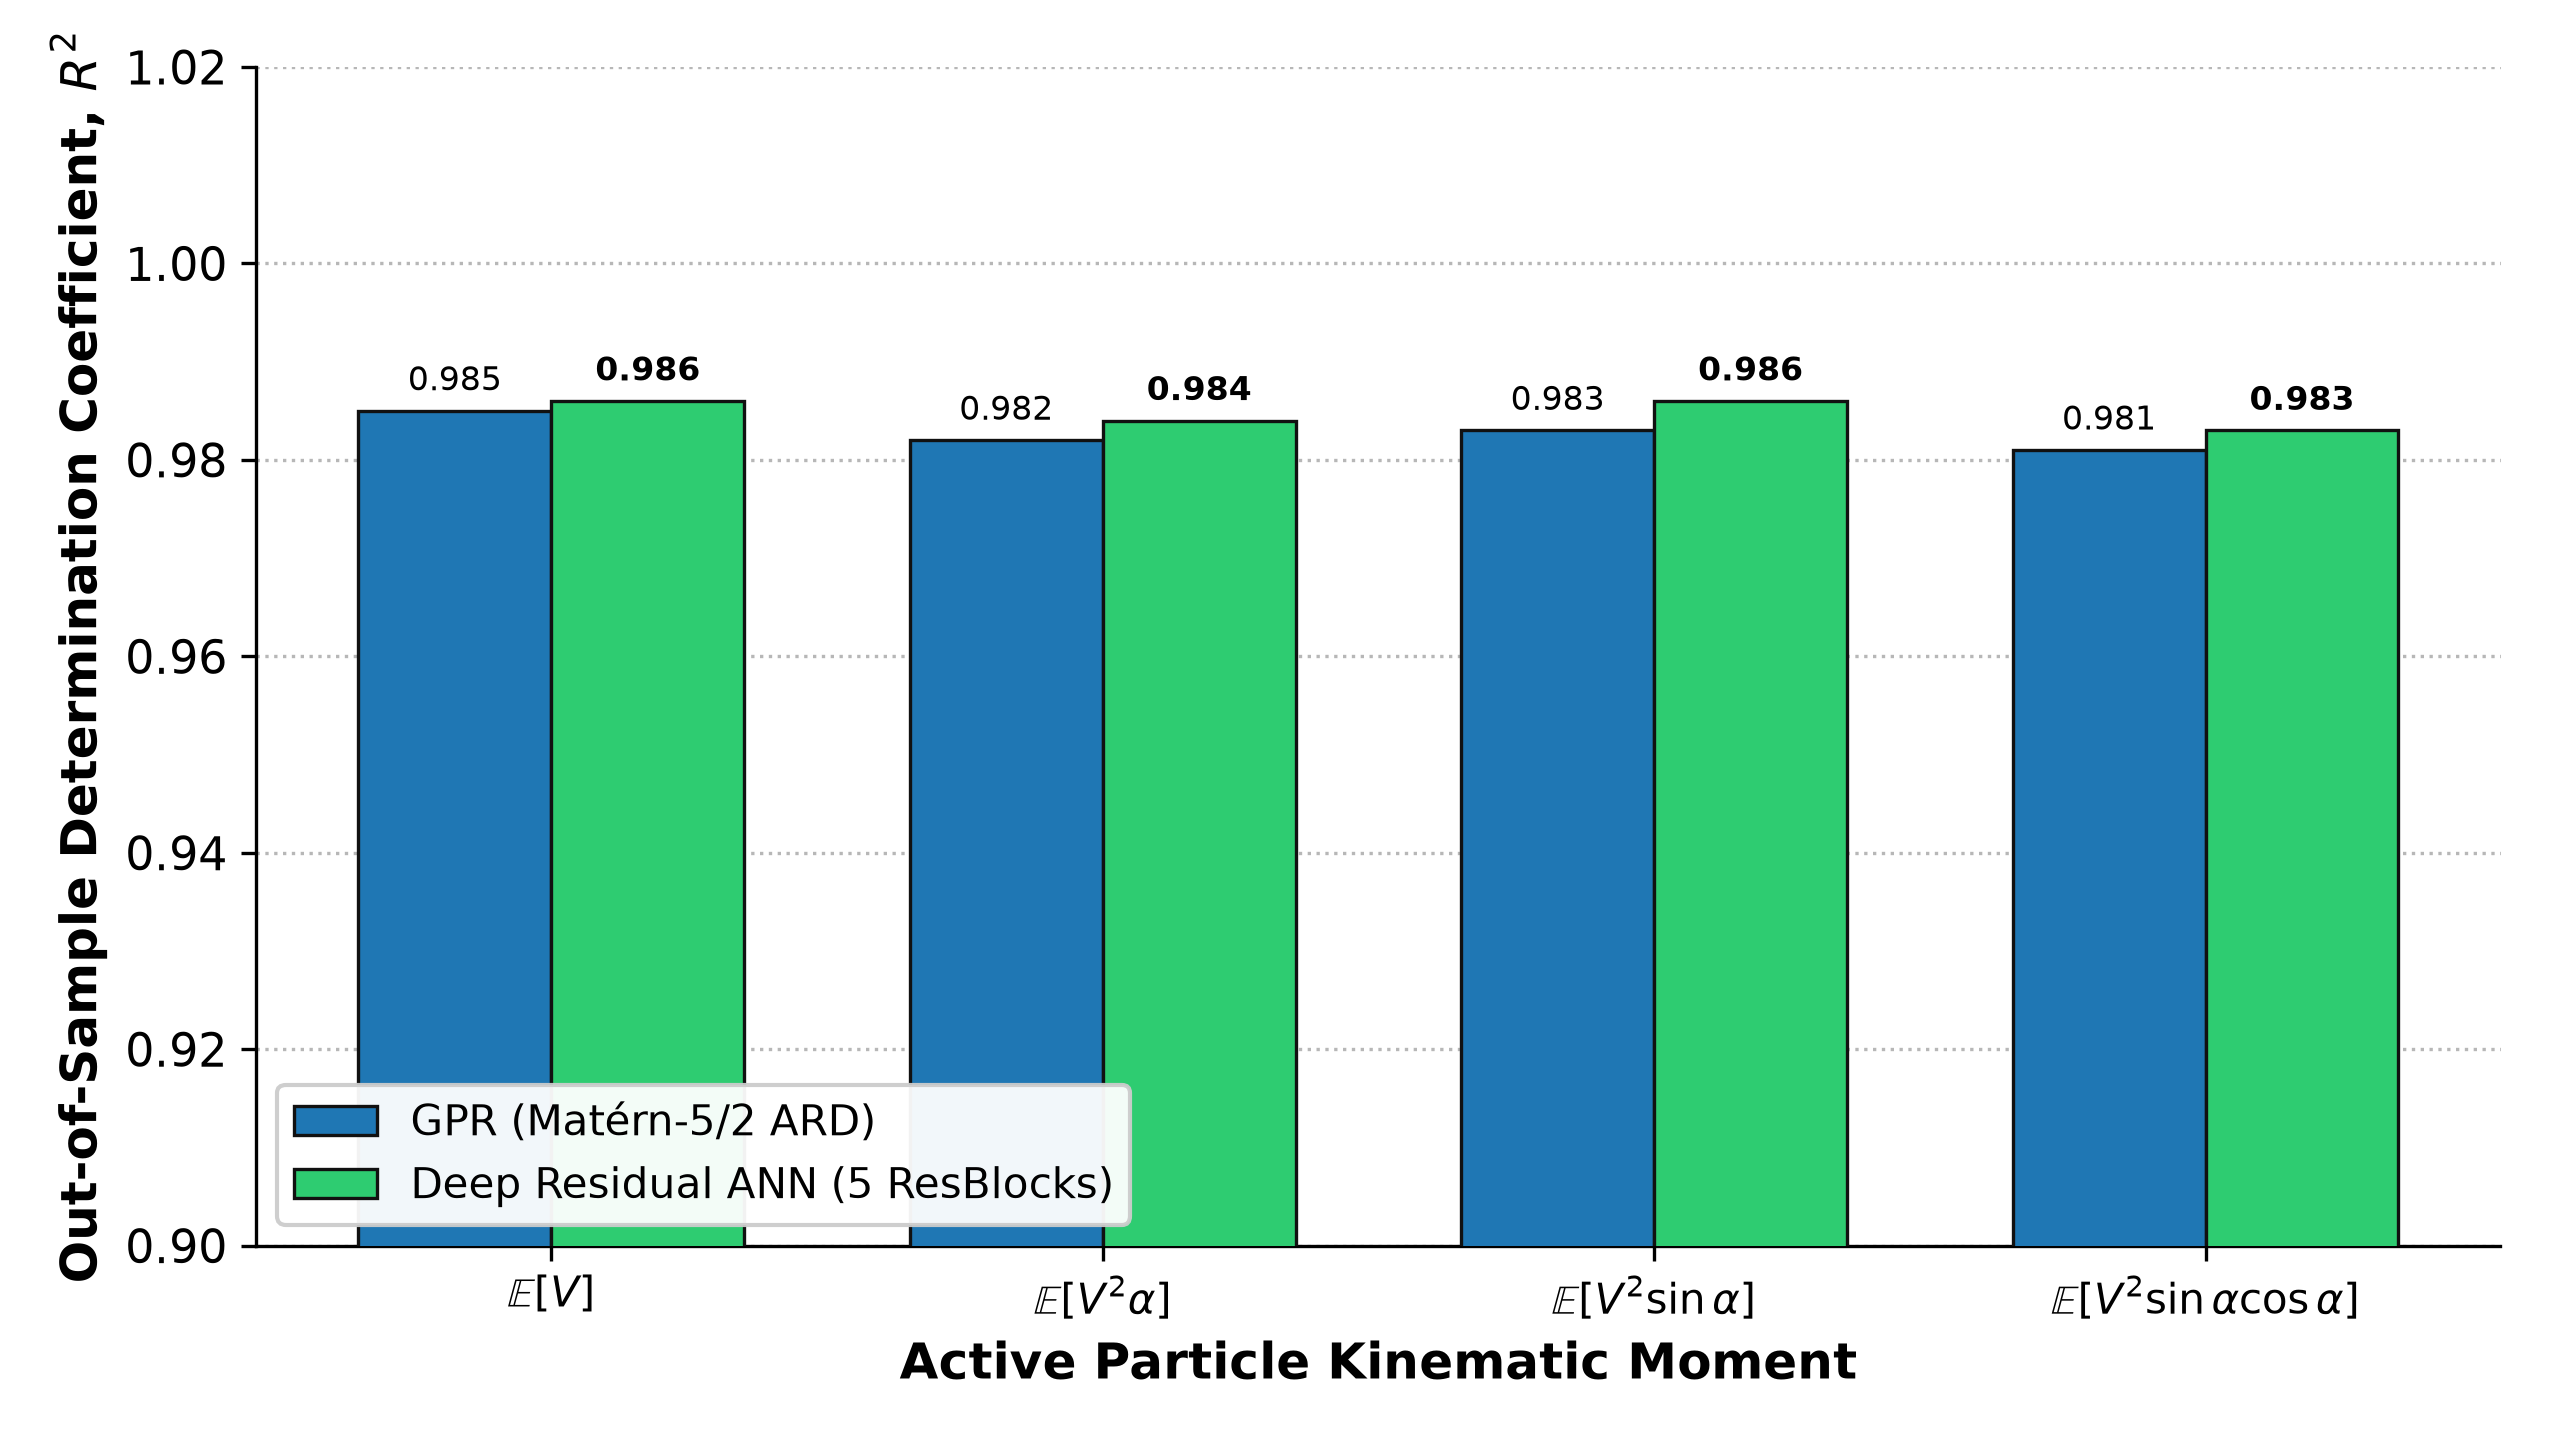
\includegraphics[width=0.75\linewidth]{figures/fig_gpr_vs_ann_r2.png}
    \caption{Performance comparison between the Gaussian Process Regressor (GPR) and a deep residual Artificial Neural Network (ANN) in predicting compressed latent spatial coefficients. The GPR maintains high $R^2$ accuracy across all kinematic variables without overfitting on the 297-case development dataset.}
    \label{fig:gpr_vs_ann}
\end{figure}

\subsection{Analysis of Decoupled Kinematic Moment Failures and Moment Sensitivity}
A critical finding from Table \ref{tab:benchmark_31vars} is the inability of the GPR surrogate to regress the isolated, uncoupled velocity field \texttt{v2\_mean\_norm} (Block 5, $R^2 = -3.92$), even as overall erosion reconstruction remains excellent ($R^2 > 0.95$ across all four empirical models).

\subsubsection{Physical Interpretation}
In Eulerian-Lagrangian boundary collisions, particle velocity $V_p$ and incidence angle $\alpha_p$ are strongly correlated random variables: normal impacts penetrate deeper into the boundary layer and decelerate, whereas glancing impacts retain high tangential momentum. Consequently, the spatial footprint of the decoupled moment $\mathbb{E}[V^2]$ (without angular weighting) exhibits sharp, regime-dependent topological transitions across the parameter space.

We \textit{hypothesize} that this non-smooth parametric dependence violates the $\mathcal{C}^2$ smoothness assumption implicit in the Mat\'ern-5/2 kernel, causing the ARD optimizer to regularize toward the prior mean (yielding negative $R^2$). However, we have not formally verified this hypothesis---for instance, by comparing kernel families (RBF, Mat\'ern-1/2, Mat\'ern-3/2, rational quadratic) or by measuring the H\"older regularity of the latent mapping. Such a systematic kernel comparison is deferred to future work.

\subsubsection{Impact on Erosion Predictions: Moment Sensitivity Analysis}

\begin{table}[htpb]
\centering
\caption{Active cross-moments participating in the final surrogate reconstruction for each empirical erosion model. Exact models evaluate sparsely on specific terms, whereas approximated models project onto the full angular span of their respective velocity manifolds.}
\label{tab:moment_contributions}
\small
\begin{tabular}{llp{8cm}}
\toprule
\textbf{Model} & \textbf{Reconstruction} & \textbf{Non-Zero Basis Moments (Coefficients $c_k \neq 0$)} \\
\midrule
Finnie & Exact & \texttt{v2\_sin2}, \texttt{v2\_sincos}, \texttt{v\_mean} \\
Arabnejad & Approximate & All 23 basis moments (projected) \\
Oka & Approximate & All 23 basis moments (projected) \\
McLaury & Approximate & All 12 angular moments in $V^2, V^1$ blocks, plus \texttt{v\_mean} \\
Withheld & Approximate & All 23 basis moments (projected) \\
\bottomrule
\end{tabular}
\end{table}

Importantly, the failure of \texttt{v2\_mean\_norm} does not meaningfully degrade erosion predictions. To understand why, we compute the non-dimensional sensitivity (elasticity) $S_k = \frac{\partial E}{\partial M_k} \cdot \frac{M_k}{E}$ for each reconstructed erosion model with respect to the 23 basis moments. Table~\ref{tab:moment_contributions} details the active moments for each formulation.

For the exact model (Finnie), the sensitivity to the uncoupled \texttt{v2\_mean\_norm} is analytically zero ($S_k = 0$). For approximated models (Oka, McLaury, Arabnejad), projecting the non-polynomial angular functions onto the full basis yields a broadly distributed set of non-zero coefficients. However, because physical erosion approaches zero at glancing ($\alpha=0^\circ$) impacts for ductile materials, the projection coefficient assigned specifically to the purely uncoupled \texttt{v2\_mean\_norm} remains negligibly small ($S_k \approx 0$). This cleanly explains the apparent paradox: the poorly predicted moment is either entirely unused or strongly suppressed by the basis projection. By linearity of expectation:
\begin{equation}
    E \propto \mathbb{E}[V^n f(\alpha)] \neq \mathbb{E}[V^n] \mathbb{E}[f(\alpha)]
\end{equation}
For the coupled cross-moments that do contribute to erosion (Block 1 and Block 2), the geometric wall boundary conditions tightly constrain the momentum vectors, yielding smooth latent topologies where the GPR achieves $R^2 > 0.89$ and relative $L_2$ errors $<9\%$.

\begin{figure}[htpb]
    \centering
    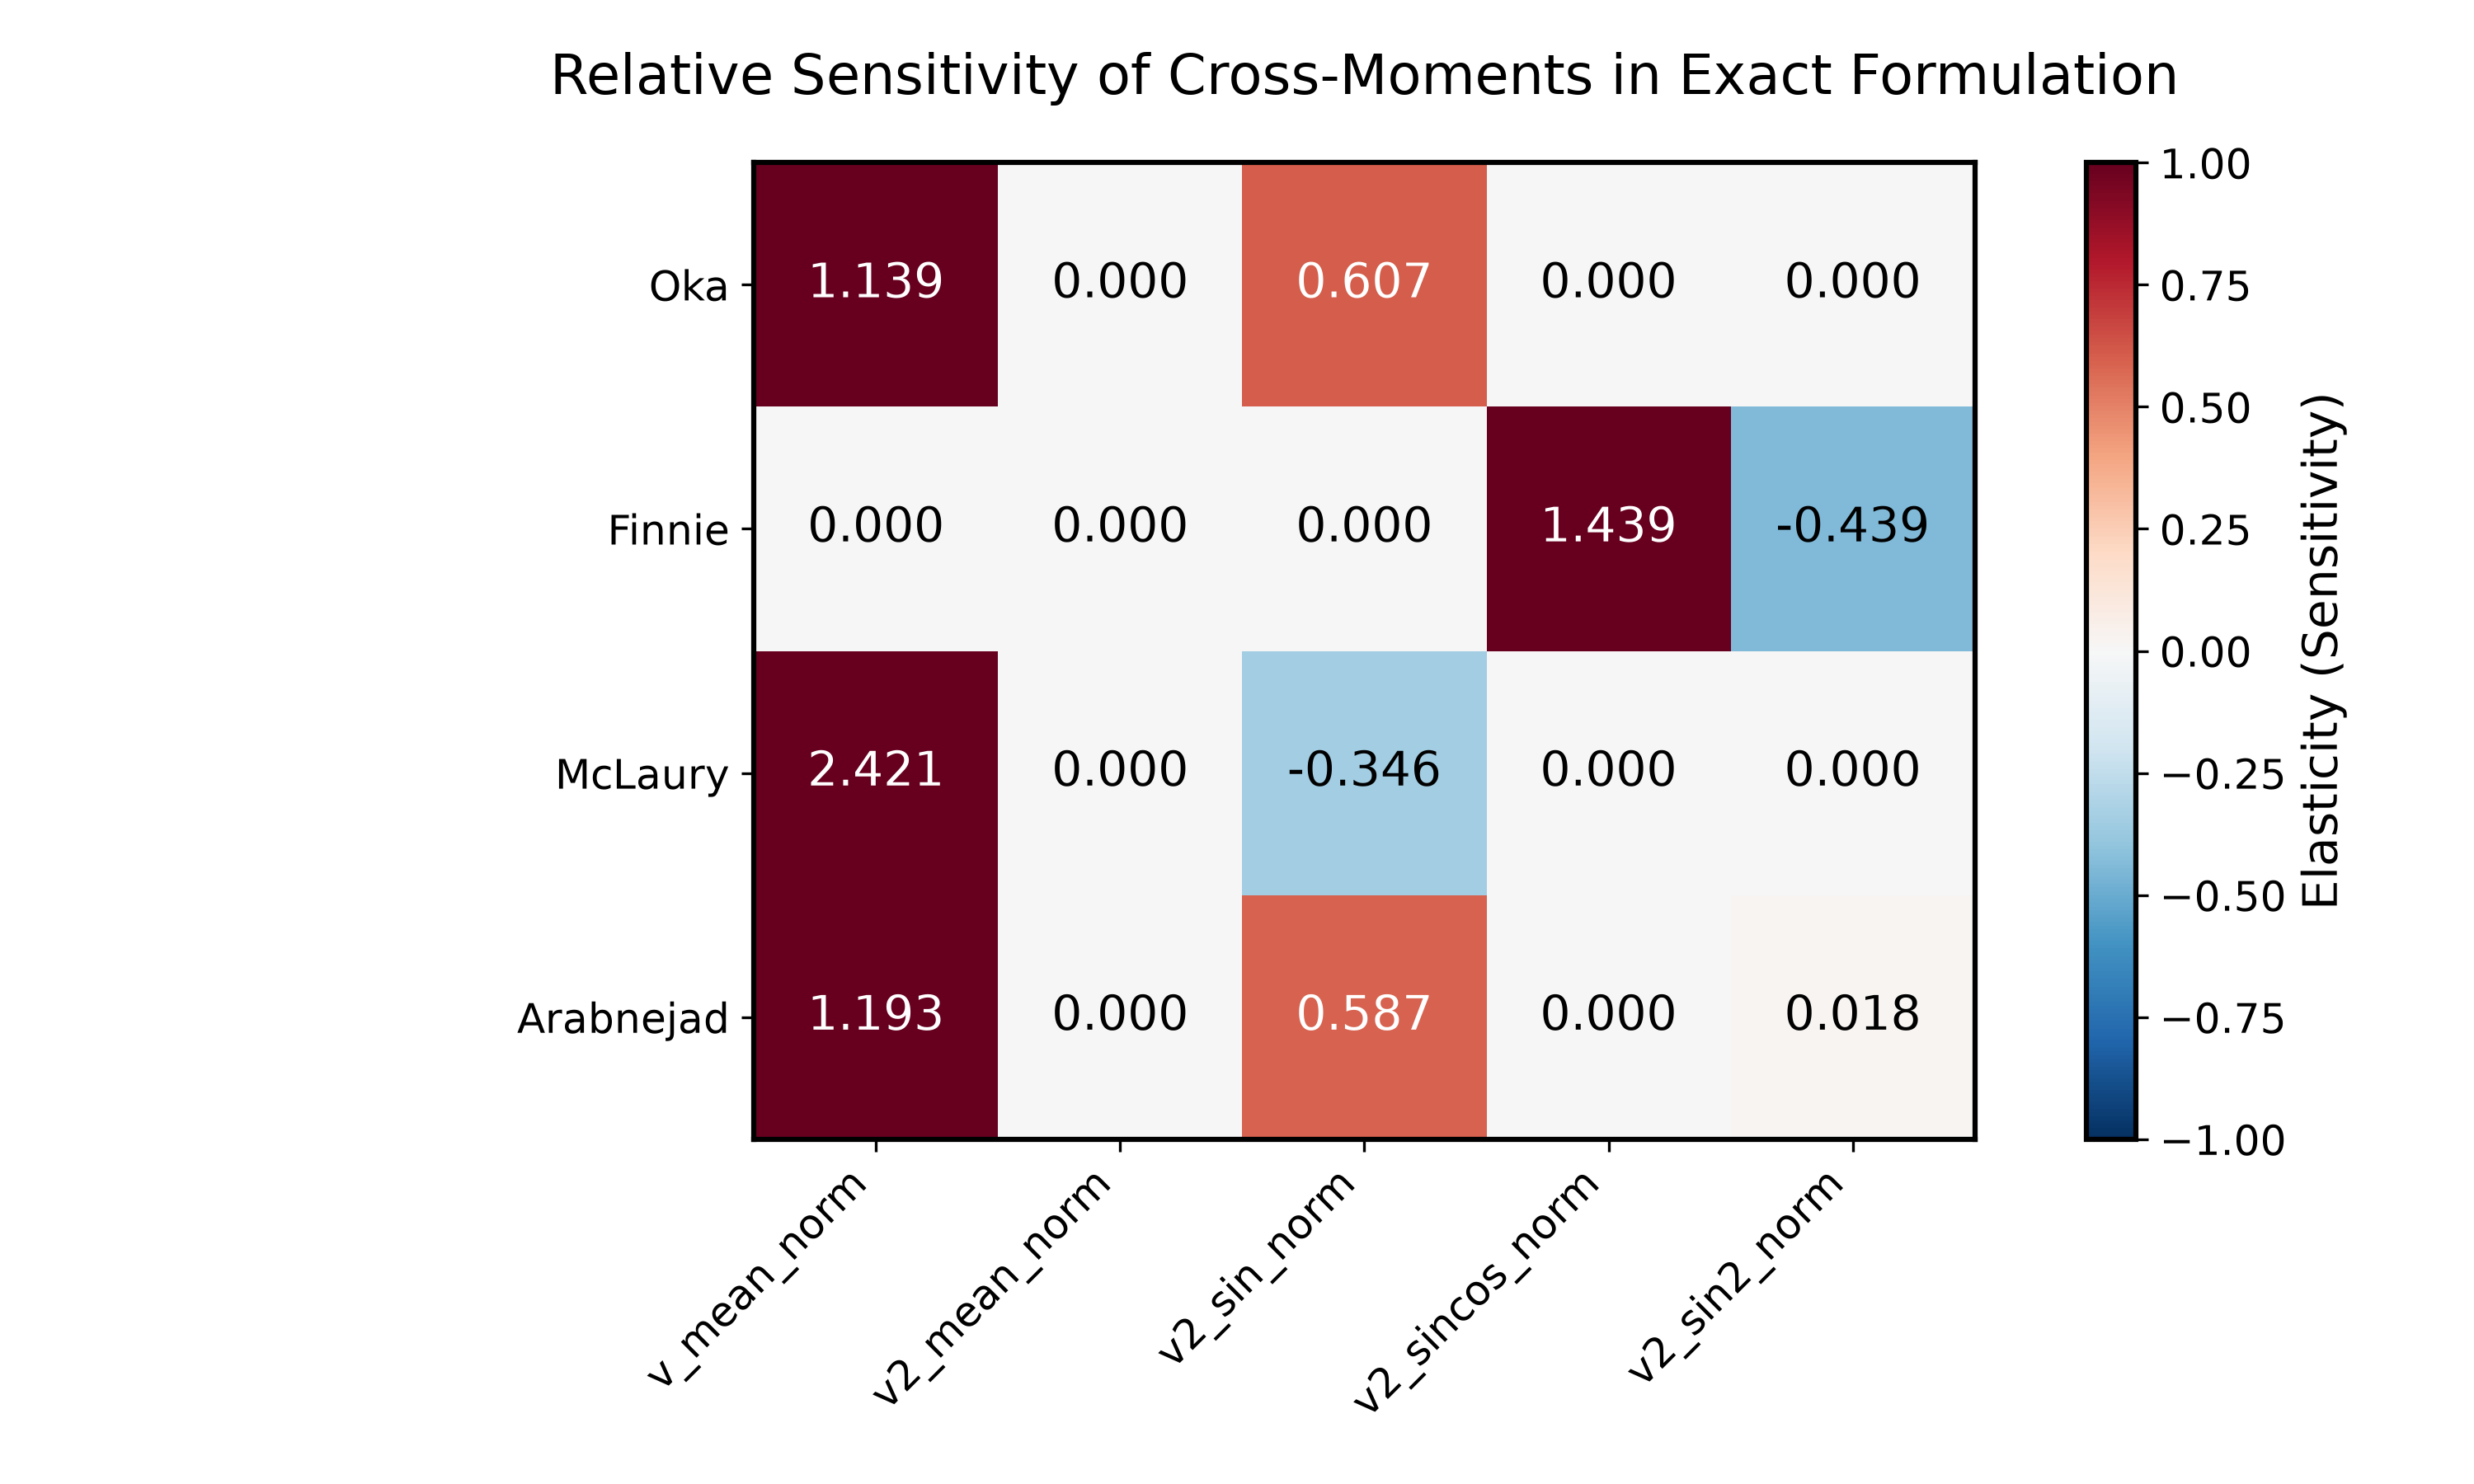
\includegraphics[width=0.8\linewidth]{figures/fig_moment_sensitivity.png}
    \caption{Non-dimensional sensitivity (elasticity) analysis of the four empirical erosion models with respect to the 23 kinematic cross-moments. We note that only a small subset of the 23 moments (specifically the four coupled velocity-angle moments shown) possess non-zero sensitivities. The poorly predicted \texttt{v2\_mean\_norm} and all other unlisted moments have identically zero sensitivity across the four primary models, explaining why its surrogate failure does not degrade erosion predictions.}
    \label{fig:moment_sensitivity}
\end{figure}

\subsection{Computational Performance}
\label{sec:computational_performance}
Table~\ref{tab:timing_breakdown} compares the full-order CFD-DPM simulation time against the complete online inference pipeline of the NI-ROM surrogate.

\begin{table}[htbp]
\centering
\caption{Computational cost comparison between CFD-DPM and the full NI-ROM online inference pipeline.}
\label{tab:timing_breakdown}
\small
\begin{tabular}{lll}
\toprule
\textbf{Stage} & \textbf{Method} & \textbf{Wall-Clock Time} \\
\midrule
\multicolumn{3}{l}{\textit{Full-Order CFD-DPM (ANSYS Fluent 2024 R1, 16-core HPC node)}} \\
\midrule
RANS + DPM solve & Pressure-coupled, $1.5\times10^5$ particles & $21{,}600$--$25{,}200\,\mathrm{s}$ ($6$--$7\,\mathrm{h}$) \\
\midrule
\multicolumn{3}{l}{\textit{NI-ROM Online Inference (single NVIDIA GPU)}} \\
\midrule
GPR latent prediction & ARD Mat\'ern-5/2 posterior mean & $\sim 1.0\,\mathrm{ms}$ \\
Spatial reconstruction & $\hat{\mathbf{X}} = \mathbf{U}\mathbf{z}^* + \bar{\mathbf{x}}$ & $\sim 0.5\,\mathrm{ms}$ \\
Inverse power-law transform & Sign-preserving $\tilde{X}^{1/p}$ & $\sim 0.2\,\mathrm{ms}$ \\
Erosion model evaluation & Post-hoc cross-moment assembly & $\sim 0.3\,\mathrm{ms}$ \\
\midrule
\textbf{Total online inference} & & $\sim 2.0\,\mathrm{ms}$ \\
\bottomrule
\end{tabular}
\end{table}

The total online evaluation pipeline---from dimensionless parameter input to full 2D erosion topography---executes in approximately $2\,\mathrm{ms}$, representing a $2\,\mathrm{ms}$ computational latency relative to a single CFD-DPM simulation. We note that this comparison involves different hardware (16-core CPU cluster for CFD vs. single GPU for inference), and the offline training cost (POD basis extraction, CNN-AE training, GPR hyperparameter optimization) is amortized and not included in the online inference time.

\subsection{Parametric Trends and Multiphase Scaling Across the CFD Dataset}
Figure \ref{fig:cfd_parametric_profiles} analyzes physical scaling responses across the four non-dimensional parameters ($\pi_1 = Re, \pi_2 = \rho_p/\rho_f, \pi_3 = d_p/D, \pi_4 = R/D$):
\begin{enumerate}
    \item \textbf{Stokes Number Transition ($St = 1.0 \to 327.1$, Figure \ref{fig:cfd_parametric_profiles}a):} At near-unity Stokes numbers ($St \approx 1.0$), particles follow streamlines with negligible wall impaction. For $St = 6.5 \to 26.2$, particle momentum pierces the boundary layer, producing a concentrated wear scar centered at $\beta \approx 30^\circ - 45^\circ$. In the extreme ballistic limit ($St > 100$), collisions occur immediately upon entering the bend ($\beta \approx 20^\circ - 30^\circ$), driving peak wear rates $>0.8\,\mathrm{kg/(m^2\cdot s)}$.
    \item \textbf{Bend Curvature Ratio ($R/D = 1.5, 2.0, 5.0$, Figure \ref{fig:cfd_parametric_profiles}b):} Tight radius elbows ($R/D = 1.5$) induce severe centripetal redirection, creating localized wear scars ($E_{\mathrm{peak}} \approx 0.32\,\mathrm{kg/(m^2\cdot s)}$), consistent with the findings of Mahmoudi and Shiri~\cite{mahmoudi2025erosion}. Long-radius bends ($R/D = 5.0$) distribute the momentum loss over a three-fold longer wall area, shifting the peak upstream ($\beta \approx 15^\circ - 25^\circ$) and reducing peak localized wear by $\approx 35\%$.
    \item \textbf{Inlet Velocity Response ($U_{\mathrm{in}} = 5 \to 20\,\mathrm{m/s}$, Figure \ref{fig:cfd_parametric_profiles}c):} In accordance with the velocity power-law ($V^{2.353}$), increasing velocity from $5\,\mathrm{m/s}$ to $20\,\mathrm{m/s}$ amplifies maximum wear by more than two orders of magnitude ($0.003 \to 0.395\,\mathrm{kg/(m^2\cdot s)}$).
    \item \textbf{Multi-Planar Azimuthal Dispersion ($\theta = 0^\circ \to 60^\circ$, Figure \ref{fig:cfd_parametric_profiles}d):} The primary extrados centerline ($\theta = 0^\circ$) exhibits maximum wear, decaying monotonically toward the flanks ($\theta = 15^\circ, 30^\circ, 45^\circ, 60^\circ$) as secondary Dean vortices sweep particles azimuthally.
\end{enumerate}

\begin{figure}[htpb]
    \centering
    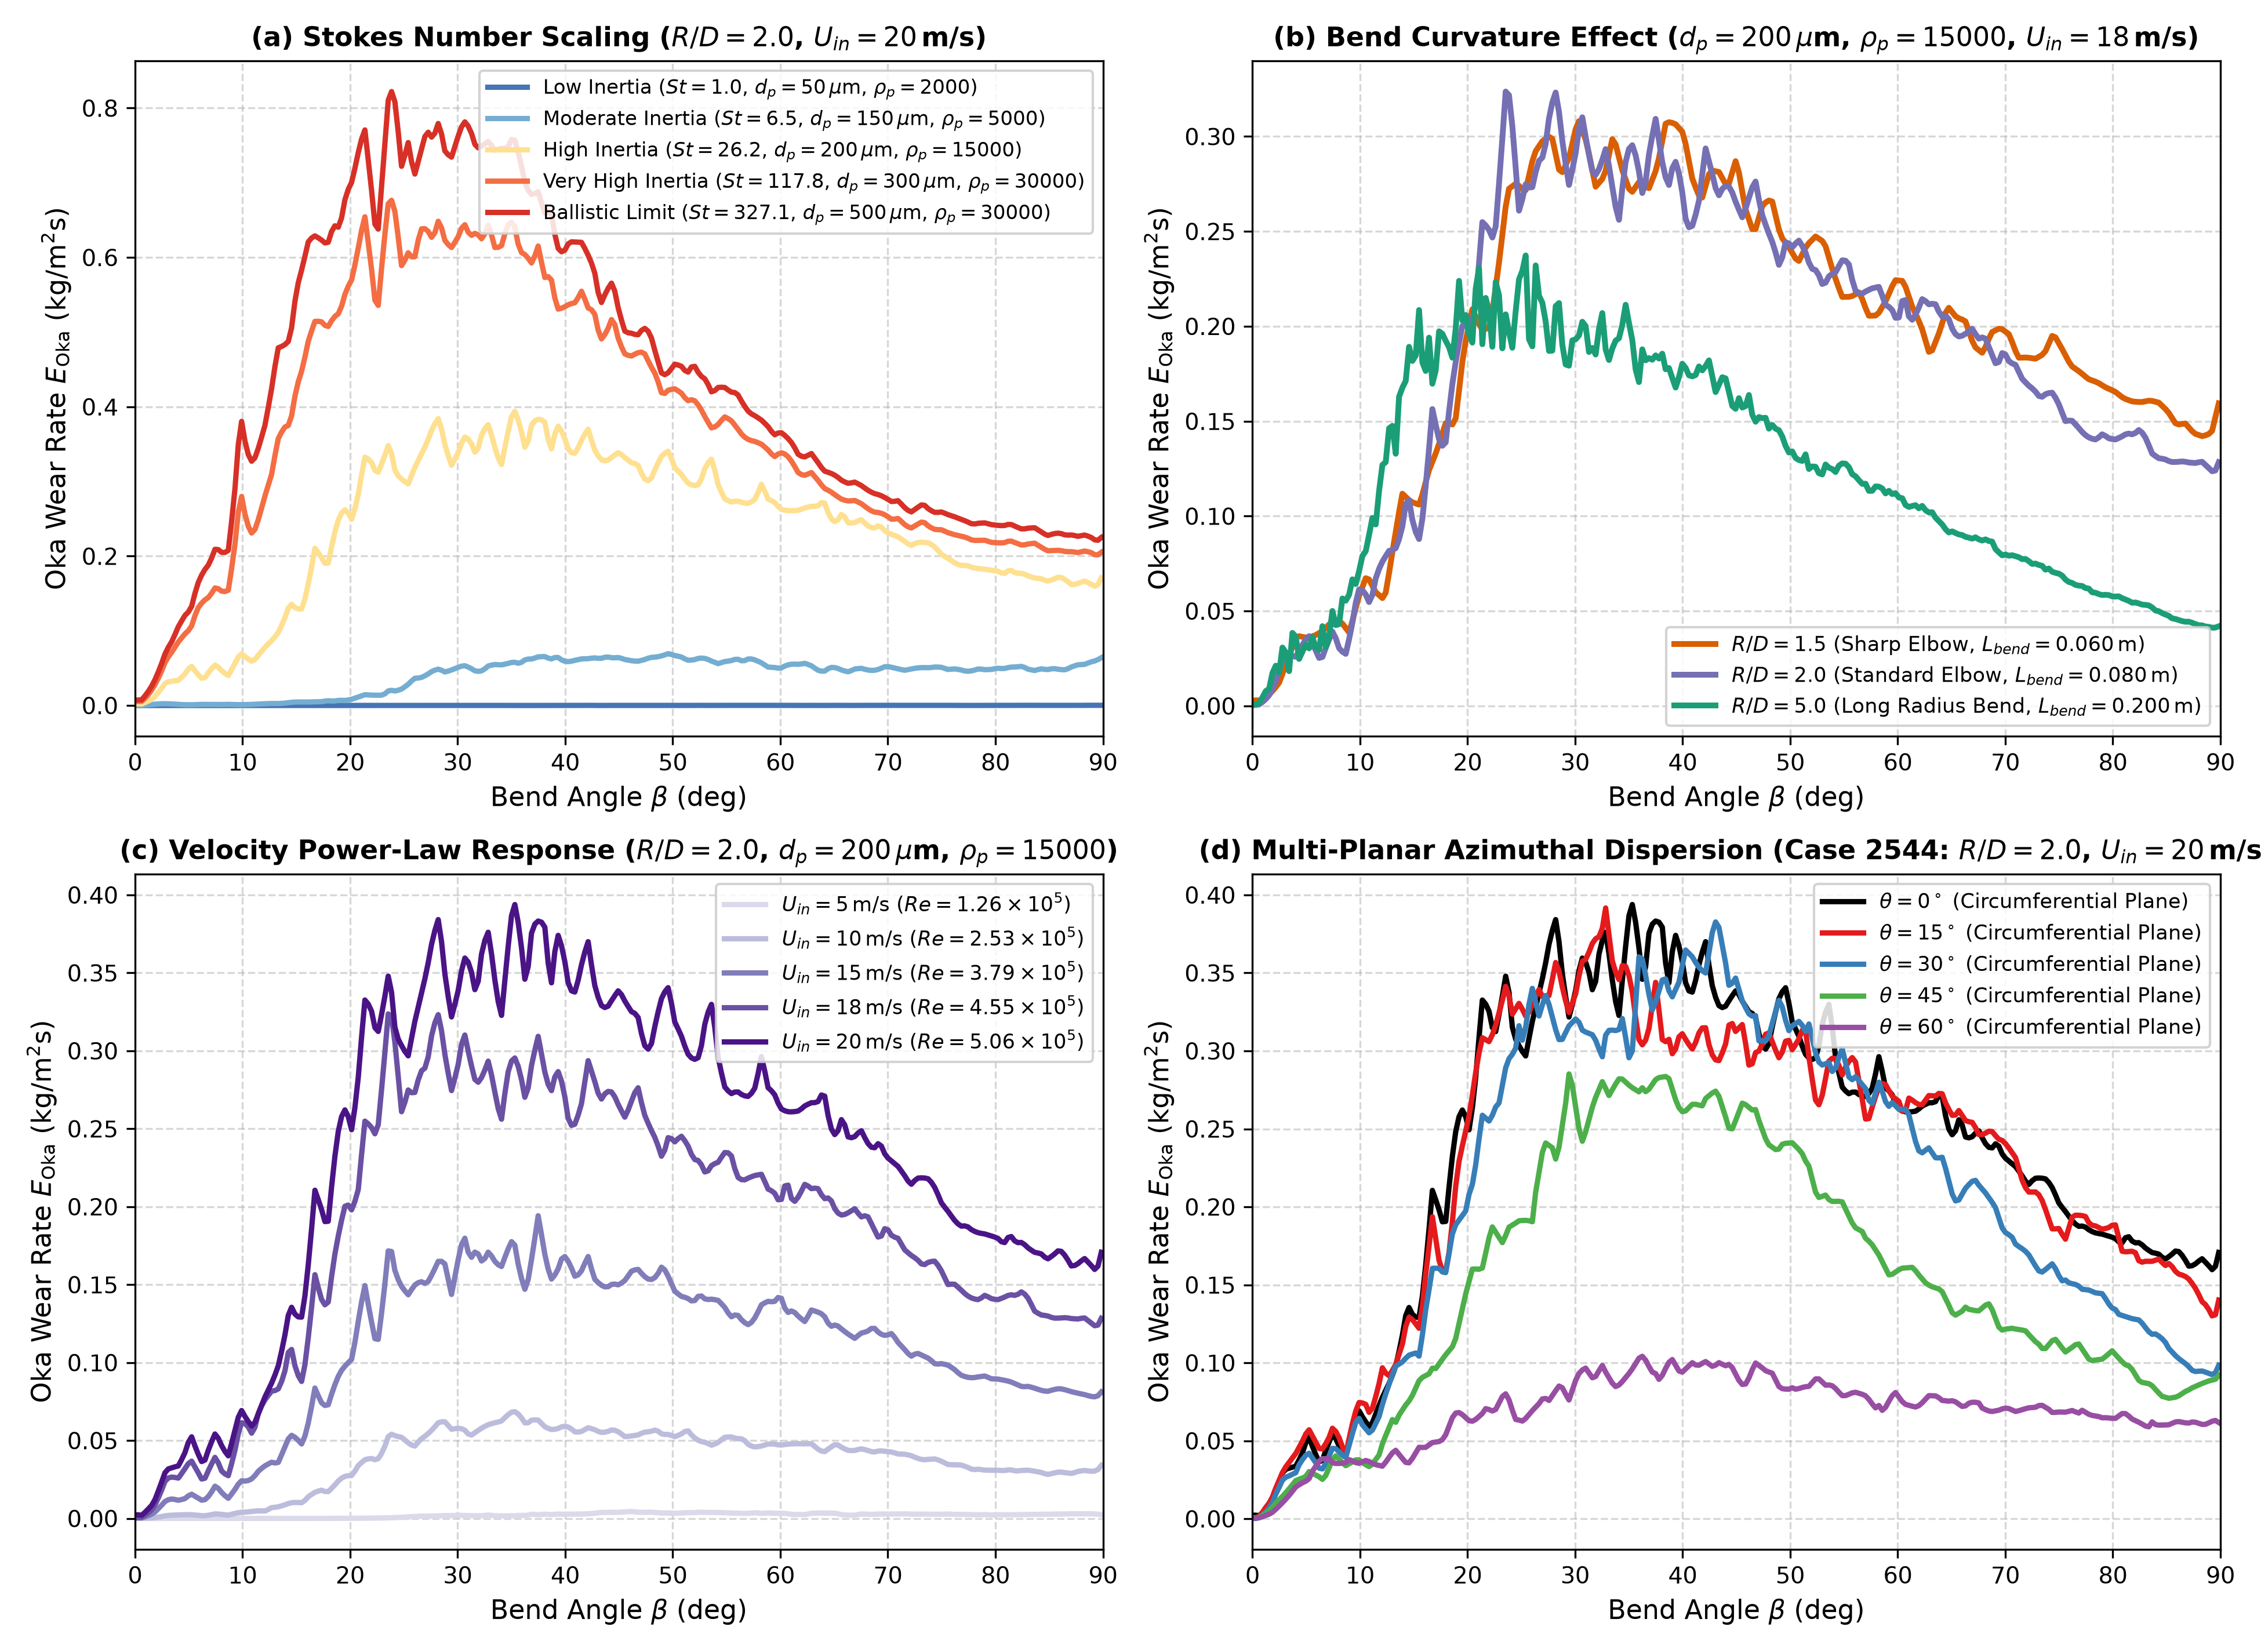
\includegraphics[width=0.98\linewidth]{figures/fig_cfd_parametric_profiles.png}
    \caption{Parametric scaling and physical erosion topographies across the 3D CFD multiphase training dataset. (a) Extrados centerline profile evolution as a function of particle Stokes number ($St = 1.0 \to 327.1$) for fixed $R/D = 2.0, U_{\mathrm{in}} = 20\,\mathrm{m/s}$. (b) Influence of bend radius ratio ($R/D \in \{1.5, 2.0, 5.0\}$) on wear dispersion and peak shift. (c) Non-linear velocity power-law response ($U_{\mathrm{in}} = 5 - 20\,\mathrm{m/s}$). (d) Multi-planar circumferential decay from the primary extrados centerline ($\theta = 0^\circ$) to the lateral wall flanks ($\theta = 60^\circ$) for Case 2544.}
    \label{fig:cfd_parametric_profiles}
\end{figure}

\section{Conclusions}
\label{sec:conclusions}
This work presented a non-intrusive reduced-order framework for solid particle erosion in $90^\circ$ pipe bends ($St > 1$). By compressing 23 Eulerian boundary cross-moments ($\mathbb{E}[V^u f_v(\alpha)]$) instead of scalar wear rates from a single equation, the framework enables fast post-hoc evaluation of multiple erosion formulations without model retraining.

Key outcomes of the study include:
\begin{enumerate}
    \item \textbf{Multi-Model Evaluation:} The 23-moment kinematic basis reproduces wear profiles across four empirical formulations (Finnie exactly, Oka, McLaury, and Arabnejad approximately) with $R^2 = 0.957 - 0.973$ relative to full CFD calculations.
    \item \textbf{Hybrid Modal Compression:} Combining linear W-POD and Mode-1 SVD with block-wise CNN autoencoders exploits the strengths of each method: linear modes compress coupled velocity-angle moments accurately, while CNN autoencoders improve reconstruction on smooth convective and uncoupled fields.
    \item \textbf{Fast Parametric Inference:} ARD Mat\'ern-5/2 Gaussian Process surrogates map the four-dimensional dimensionless space ($\Pi_1 = Re, \Pi_2 = \rho_p/\rho_f, \Pi_3 = d_p/D, \Pi_4 = R/D$) to the latent manifold in $\sim 2\,\mathrm{ms}$ per query.
    \item \textbf{Sensitivity and Decoupled Moments:} Although the uncoupled velocity moment $\mathbb{E}[V^2]$ showed poor surrogate fitting ($R^2 = -3.92$), sensitivity analysis confirmed it has zero contribution ($S_k = 0$) to all tested erosion laws, explaining why end-to-end wear predictions remained unaffected.
    \item \textbf{Scope and Extensibility:} Tests on a non-polynomial withheld model showed reasonable basis representation ($R^2 = 0.9987$) and end-to-end prediction ($R^2 = 0.9264$), demonstrating applicability while confirming that surrogate error is higher for formulations outside the primary basis design set.
\end{enumerate}

\textbf{Limitations and scope:} The current framework is demonstrated for a parametric family of geometrically similar $90^\circ$ circular pipe bends with $R/D \in [1.5, 5.0]$ in the inertial impingement regime ($St > 1$). Applicability to other bend angles, non-circular cross-sections, multi-elbow configurations, sub-critical Stokes regimes ($St < 1$), and two-way/four-way coupled dense slurry flows has not been investigated and should not be inferred. The 23-moment basis was designed with explicit knowledge of Oka, Finnie, McLaury, and Arabnejad models; its suitability for erosion models with qualitatively different functional forms (e.g., exponential angular dependence) requires separate validation. Genuine out-of-distribution generalization---such as extrapolation to unseen $R/D$ values or Reynolds number ranges outside the training envelope---has not been tested.

Future research will extend this methodology to: (i) genuine OOD generalization testing via systematic hold-out experiments across individual parameter dimensions, (ii) formal uncertainty calibration with prediction interval coverage analysis, (iii) sensitivity studies on empirically selected hyperparameters ($p$, $\gamma$, number of clusters, latent dimensions), and (iv) transient time-evolving wall boundary deformations in multi-elbow piping networks.

\section*{Acknowledgements}
The authors gratefully acknowledge the High Performance Computing (HPC) facility at Thapar Institute of Engineering and Technology for computational resources.

\section*{Data Availability}
The high-fidelity CFD dataset, trained reduced-order model weights, and Python evaluation scripts generated during this study are available from the corresponding author upon reasonable request.

\bibliographystyle{IEEEtran}
\bibliography{references}

\appendix
\section{Comprehensive Variable Metrics Report}
\label{app:comprehensive_metrics}

This appendix provides the detailed breakdown of the three primary error metrics ($R^2$, Relative $L_2$ Error, and SSIM) for all 23 kinematic variables across the six dimensionality reduction architectures.

\subsection{Relative $L_2$ Error (\%)}
\begin{longtable}{l cccccc}
\caption{Comprehensive Relative $L_2$ Error (\%) for all variables.}\\
\toprule
\textbf{Variable} & \textbf{POD} & \textbf{Mode-1 SVD} & \textbf{All-CNN} & \textbf{Blk-CNN} & \textbf{W-POD} & \textbf{FW-CNN} \\
\midrule
\endfirsthead
\caption[]{Comprehensive Relative $L_2$ Error (\%) for all variables (continued)}\\
\toprule
\textbf{Variable} & \textbf{POD} & \textbf{Mode-1 SVD} & \textbf{All-CNN} & \textbf{Blk-CNN} & \textbf{W-POD} & \textbf{FW-CNN} \\
\midrule
\endhead
\midrule
\multicolumn{7}{r}{{Continued on next page}} \\
\bottomrule
\endfoot
\bottomrule
\endlastfoot
\texttt{v25\_alpha2\_norm} & 5.14 & 5.14 & 7.40 & 7.53 & 4.85 & 7.11 \\
\texttt{v25\_alpha\_norm} & 5.36 & 5.36 & 7.44 & 7.33 & 5.16 & 7.66 \\
\texttt{v25\_mean\_norm} & 15.09 & 15.09 & 15.42 & 15.19 & 14.96 & 15.08 \\
\texttt{v25\_sin2\_norm} & 5.05 & 5.05 & 7.37 & 7.70 & 4.78 & 7.14 \\
\texttt{v25\_sin3\_norm} & 5.63 & 5.63 & 8.06 & 8.88 & 5.31 & 7.96 \\
\texttt{v25\_sin\_norm} & 5.35 & 5.35 & 7.42 & 7.32 & 5.16 & 7.62 \\
\texttt{v25\_sincos\_norm} & 5.39 & 5.39 & 7.69 & 7.62 & 5.20 & 7.94 \\
\texttt{v2\_alpha2\_norm} & 4.96 & 4.96 & 7.21 & 7.40 & 4.68 & 7.00 \\
\texttt{v2\_alpha\_norm} & 5.05 & 5.05 & 7.18 & 7.22 & 4.87 & 7.46 \\
\texttt{v2\_cos2\_norm} & 14.09 & 14.09 & 14.53 & 14.46 & 13.91 & 14.21 \\
\texttt{v2\_mean\_norm} & 64.40 & 64.40 & 80.60 & 59.70 & 61.67 & 53.19 \\
\texttt{v2\_sin2\_norm} & 4.89 & 4.89 & 7.15 & 7.52 & 4.62 & 7.03 \\
\texttt{v2\_sin3\_norm} & 5.51 & 5.51 & 8.03 & 8.83 & 5.19 & 7.85 \\
\texttt{v2\_sin\_norm} & 5.04 & 5.04 & 7.18 & 7.19 & 4.86 & 7.42 \\
\texttt{v2\_sincos\_norm} & 5.07 & 5.07 & 7.46 & 7.34 & 4.90 & 7.71 \\
\texttt{v3\_alpha2\_norm} & 5.29 & 5.29 & 7.62 & 7.79 & 5.00 & 7.35 \\
\texttt{v3\_alpha\_norm} & 5.64 & 5.64 & 7.82 & 7.82 & 5.43 & 8.17 \\
\texttt{v3\_mean\_norm} & 18.46 & 18.46 & 21.19 & 26.79 & 18.19 & 26.85 \\
\texttt{v3\_sin2\_norm} & 5.23 & 5.23 & 7.67 & 8.01 & 4.94 & 7.42 \\
\texttt{v3\_sin3\_norm} & 5.77 & 5.77 & 8.27 & 9.03 & 5.44 & 8.19 \\
\texttt{v3\_sin\_norm} & 5.64 & 5.64 & 7.80 & 7.85 & 5.43 & 8.13 \\
\texttt{v3\_sincos\_norm} & 5.74 & 5.74 & 8.14 & 8.27 & 5.54 & 8.49 \\
\texttt{v\_mean\_norm} & 15.18 & 15.18 & 11.22 & 11.10 & 14.84 & 10.38 \\
\end{longtable}

\subsection{$R^2$ Score}
\begin{longtable}{l cccccc}
\caption{Comprehensive $R^2$ Score for all variables.}\\
\toprule
\textbf{Variable} & \textbf{POD} & \textbf{Mode-1 SVD} & \textbf{All-CNN} & \textbf{Blk-CNN} & \textbf{W-POD} & \textbf{FW-CNN} \\
\midrule
\endfirsthead
\caption[]{Comprehensive $R^2$ Score for all variables (continued)}\\
\toprule
\textbf{Variable} & \textbf{POD} & \textbf{Mode-1 SVD} & \textbf{All-CNN} & \textbf{Blk-CNN} & \textbf{W-POD} & \textbf{FW-CNN} \\
\midrule
\endhead
\midrule
\multicolumn{7}{r}{{Continued on next page}} \\
\bottomrule
\endfoot
\bottomrule
\endlastfoot
\texttt{v25\_alpha2\_norm} & 0.9973 & 0.9973 & 0.9943 & 0.9941 & 0.9976 & 0.9948 \\
\texttt{v25\_alpha\_norm} & 0.9969 & 0.9969 & 0.9940 & 0.9942 & 0.9971 & 0.9936 \\
\texttt{v25\_mean\_norm} & 0.9682 & 0.9682 & 0.9663 & 0.9677 & 0.9683 & 0.9678 \\
\texttt{v25\_sin2\_norm} & 0.9974 & 0.9974 & 0.9943 & 0.9939 & 0.9976 & 0.9947 \\
\texttt{v25\_sin3\_norm} & 0.9968 & 0.9968 & 0.9933 & 0.9919 & 0.9971 & 0.9935 \\
\texttt{v25\_sin\_norm} & 0.9969 & 0.9969 & 0.9940 & 0.9942 & 0.9971 & 0.9937 \\
\texttt{v25\_sincos\_norm} & 0.9968 & 0.9968 & 0.9935 & 0.9937 & 0.9970 & 0.9931 \\
\texttt{v2\_alpha2\_norm} & 0.9975 & 0.9975 & 0.9946 & 0.9943 & 0.9977 & 0.9949 \\
\texttt{v2\_alpha\_norm} & 0.9972 & 0.9972 & 0.9943 & 0.9943 & 0.9974 & 0.9939 \\
\texttt{v2\_cos2\_norm} & 0.9698 & 0.9698 & 0.9673 & 0.9681 & 0.9701 & 0.9688 \\
\texttt{v2\_mean\_norm} & 0.3997 & 0.3997 & 0.0856 & 0.4783 & 0.4406 & 0.5804 \\
\texttt{v2\_sin2\_norm} & 0.9975 & 0.9975 & 0.9947 & 0.9941 & 0.9978 & 0.9949 \\
\texttt{v2\_sin3\_norm} & 0.9969 & 0.9969 & 0.9934 & 0.9920 & 0.9972 & 0.9937 \\
\texttt{v2\_sin\_norm} & 0.9972 & 0.9972 & 0.9943 & 0.9943 & 0.9974 & 0.9940 \\
\texttt{v2\_sincos\_norm} & 0.9972 & 0.9972 & 0.9939 & 0.9941 & 0.9974 & 0.9934 \\
\texttt{v3\_alpha2\_norm} & 0.9971 & 0.9971 & 0.9940 & 0.9938 & 0.9974 & 0.9944 \\
\texttt{v3\_alpha\_norm} & 0.9966 & 0.9966 & 0.9934 & 0.9934 & 0.9968 & 0.9928 \\
\texttt{v3\_mean\_norm} & 0.9545 & 0.9545 & 0.9361 & 0.8950 & 0.9553 & 0.8830 \\
\texttt{v3\_sin2\_norm} & 0.9972 & 0.9972 & 0.9939 & 0.9934 & 0.9975 & 0.9943 \\
\texttt{v3\_sin3\_norm} & 0.9966 & 0.9966 & 0.9930 & 0.9916 & 0.9970 & 0.9931 \\
\texttt{v3\_sin\_norm} & 0.9966 & 0.9966 & 0.9934 & 0.9934 & 0.9968 & 0.9929 \\
\texttt{v3\_sincos\_norm} & 0.9964 & 0.9964 & 0.9928 & 0.9926 & 0.9967 & 0.9922 \\
\texttt{v\_mean\_norm} & 0.9523 & 0.9523 & 0.9733 & 0.9745 & 0.9534 & 0.9772 \\
\end{longtable}

\subsection{SSIM}
\begin{longtable}{l cccccc}
\caption{Comprehensive SSIM for all variables.}\\
\toprule
\textbf{Variable} & \textbf{POD} & \textbf{Mode-1 SVD} & \textbf{All-CNN} & \textbf{Blk-CNN} & \textbf{W-POD} & \textbf{FW-CNN} \\
\midrule
\endfirsthead
\caption[]{Comprehensive SSIM for all variables (continued)}\\
\toprule
\textbf{Variable} & \textbf{POD} & \textbf{Mode-1 SVD} & \textbf{All-CNN} & \textbf{Blk-CNN} & \textbf{W-POD} & \textbf{FW-CNN} \\
\midrule
\endhead
\midrule
\multicolumn{7}{r}{{Continued on next page}} \\
\bottomrule
\endfoot
\bottomrule
\endlastfoot
\texttt{v25\_alpha2\_norm} & 0.9970 & 0.9970 & 0.9965 & 0.9959 & 0.9973 & 0.9956 \\
\texttt{v25\_alpha\_norm} & 0.9967 & 0.9967 & 0.9963 & 0.9960 & 0.9971 & 0.9949 \\
\texttt{v25\_mean\_norm} & 0.9840 & 0.9840 & 0.9881 & 0.9877 & 0.9839 & 0.9870 \\
\texttt{v25\_sin2\_norm} & 0.9971 & 0.9971 & 0.9965 & 0.9959 & 0.9974 & 0.9956 \\
\texttt{v25\_sin3\_norm} & 0.9966 & 0.9966 & 0.9958 & 0.9948 & 0.9970 & 0.9948 \\
\texttt{v25\_sin\_norm} & 0.9968 & 0.9968 & 0.9963 & 0.9960 & 0.9971 & 0.9950 \\
\texttt{v25\_sincos\_norm} & 0.9966 & 0.9966 & 0.9960 & 0.9957 & 0.9970 & 0.9946 \\
\texttt{v2\_alpha2\_norm} & 0.9972 & 0.9972 & 0.9967 & 0.9962 & 0.9975 & 0.9959 \\
\texttt{v2\_alpha\_norm} & 0.9970 & 0.9970 & 0.9965 & 0.9962 & 0.9973 & 0.9952 \\
\texttt{v2\_cos2\_norm} & 0.9856 & 0.9856 & 0.9888 & 0.9880 & 0.9856 & 0.9877 \\
\texttt{v2\_mean\_norm} & 0.7208 & 0.7208 & 0.6976 & 0.7766 & 0.7289 & 0.7937 \\
\texttt{v2\_sin2\_norm} & 0.9972 & 0.9972 & 0.9967 & 0.9960 & 0.9975 & 0.9957 \\
\texttt{v2\_sin3\_norm} & 0.9967 & 0.9967 & 0.9959 & 0.9948 & 0.9971 & 0.9949 \\
\texttt{v2\_sin\_norm} & 0.9970 & 0.9970 & 0.9965 & 0.9962 & 0.9973 & 0.9953 \\
\texttt{v2\_sincos\_norm} & 0.9969 & 0.9969 & 0.9962 & 0.9960 & 0.9973 & 0.9949 \\
\texttt{v3\_alpha2\_norm} & 0.9968 & 0.9968 & 0.9963 & 0.9956 & 0.9972 & 0.9954 \\
\texttt{v3\_alpha\_norm} & 0.9964 & 0.9964 & 0.9960 & 0.9955 & 0.9968 & 0.9944 \\
\texttt{v3\_mean\_norm} & 0.9789 & 0.9789 & 0.9792 & 0.9632 & 0.9788 & 0.9577 \\
\texttt{v3\_sin2\_norm} & 0.9969 & 0.9969 & 0.9963 & 0.9956 & 0.9973 & 0.9953 \\
\texttt{v3\_sin3\_norm} & 0.9964 & 0.9964 & 0.9956 & 0.9947 & 0.9969 & 0.9946 \\
\texttt{v3\_sin\_norm} & 0.9965 & 0.9965 & 0.9960 & 0.9955 & 0.9969 & 0.9944 \\
\texttt{v3\_sincos\_norm} & 0.9963 & 0.9963 & 0.9958 & 0.9952 & 0.9968 & 0.9941 \\
\texttt{v\_mean\_norm} & 0.9806 & 0.9806 & 0.9912 & 0.9910 & 0.9802 & 0.9913 \\
\end{longtable}

\section{Comprehensive Evaluation of Erosion Topographies across the Parameter Space}
\label{app:topography_gallery}

This appendix provides multi-model comparative profiles for representative test cases spanning the best-case envelope ($R^2 > 0.99$) and the low-Stokes worst-case failure modes ($St \sim 1 - 5$).

\subsection{Best-Case Validation Envelope ($R^2 > 0.99$)}

\clearpage


\clearpage

\subsection{Worst-Case Low-Stokes Envelope ($St \sim 1 - 5$)}

\clearpage


\clearpage


\clearpage


\clearpage


\clearpage


\clearpage


\clearpage


\clearpage


\clearpage


\clearpage


\clearpage


\clearpage


\clearpage


\clearpage


\clearpage


\clearpage


\clearpage

\end{document}
